%
% Template Laporan Skripsi/Thesis 
%
% @author  Andreas Febrian, Lia Sadita 
% @version 1.03
%
% Dokumen ini dibuat berdasarkan standar IEEE dalam membuat class untuk 
% LaTeX dan konfigurasi LaTeX yang digunakan Fahrurrozi Rahman ketika 
% membuat laporan skripsi. Konfigurasi yang lama telah disesuaikan dengan 
% aturan penulisan thesis yang dikeluarkan UI pada tahun 2008.
%

%
% Tipe dokumen adalah report dengan satu kolom. 
%
\documentclass[12pt, a4paper, onecolumn, oneside, final]{report}

% Load konfigurasi LaTeX untuk tipe laporan thesis
\usepackage{uithesis}
\usepackage{natbib}
\usepackage{import}

\usepackage{subcaption}
\usepackage{rotating}
\usepackage{tikz}
\usepackage{amsmath}
\usepackage{amsfonts}
\usepackage{amssymb}
\usepackage[]{algorithm2e}
\usepackage{url}
\usepackage{nameref}
\usepackage{cleveref}
% \usepackage{algorithm}
\usepackage{framed}
\usepackage{listings}
\usepackage{rotating}
\usepackage{tikz}
\usepackage{pdflscape}

\usepackage{graphicx} % for pdf, bitmapped graphics files
\graphicspath{{./pics/}}
\DeclareGraphicsExtensions{.pdf,.jpeg,.png,.jpg}
% \usepackage{subfigure}

% Load konfigurasi khusus untuk laporan yang sedang dibuat
%-----------------------------------------------------------------------------%
% Informasi Mengenai Dokumen
%-----------------------------------------------------------------------------%
% 
% Judul laporan. 
\var{\judul}{Pemilihan Segmen dari Berbagai Segmentasi untuk Segmentasi Semantik Berdasarkan \textit{Conditional Random Field} melalui \textit{Latent Dirichlet Allocation} dan Algoritme Genetika}% 

% Tulis kembali judul laporan, kali ini akan diubah menjadi huruf kapital
\Var{\Judul}{Pemilihan Segmen dari Berbagai Segmentasi untuk Segmentasi Semantik Berdasarkan \textit{Conditional Random Field} melalui \textit{Latent Dirichlet Allocation} dan Algoritme Genetika}%
 
% Tulis kembali judul laporan namun dengan bahasa Ingris
\var{\judulInggris}{Selecting Segments from Multiple Segmentatation for Conditional Random Field based Semantic Segmentation via Latent Dirichlet Allocation and Genetic Algorithm}

% 
% Tipe laporan, dapat berisi Skripsi, Tugas Akhir, Thesis, atau Disertasi
\var{\type}{Skripsi}
% 
% Tulis kembali tipe laporan, kali ini akan diubah menjadi huruf kapital
\Var{\Type}{Skripsi}
% 
% Tulis nama penulis 
\var{\penulis}{Jogie Chandra}
% 
% Tulis kembali nama penulis, kali ini akan diubah menjadi huruf kapital
\Var{\Penulis}{Jogie Chandra}
% 
% Tulis NPM penulis
\var{\npm}{1106053640}
% 
% Tuliskan Fakultas dimana penulis berada
\Var{\Fakultas}{Ilmu Komputer}
\var{\fakultas}{Ilmu Komputer}
% 
% Tuliskan Program Studi yang diambil penulis
\Var{\Program}{Ilmu Komputer}
\var{\program}{Ilmu Komputer}
\var{\programEng}{Computer Science}
% 
% Tuliskan tahun publikasi laporan
\Var{\bulanTahun}{Desember 2014}
% 
% Tuliskan gelar yang akan diperoleh dengan menyerahkan laporan ini
\var{\gelar}{Sarjana Ilmu Komputer}
% 
% Tuliskan tanggal pengesahan laporan, waktu dimana laporan diserahkan ke 
% penguji/sekretariat
\var{\tanggalPengesahan}{24 Desember 2014} 
% 
% Tuliskan tanggal keputusan sidang dikeluarkan dan penulis dinyatakan 
% lulus/tidak lulus
\var{\tanggalLulus}{8 Januari 2015}
% 
% Tuliskan pembimbing 
\var{\pembimbing}{Wisnu Jatmiko, S.T., M.Kom., Dr. Eng.}
%\var{\pembimbingdua}{Dia S.Kom, M.Kom}
% 
% Alias untuk memudahkan alur penulisan paa saat menulis laporan
\var{\saya}{Penulis}

%-----------------------------------------------------------------------------%
% Judul Setiap Bab
%-----------------------------------------------------------------------------%
% 
% Berikut ada judul-judul setiap bab. 
% Silahkan diubah sesuai dengan kebutuhan. 
% 
\Var{\kataPengantar}{Kata Pengantar}
\Var{\babSatu}{Pendahuluan}
\Var{\babDua}{Landasan Teori}
\Var{\babTiga}{Metode Usulan}
% \Var{\babEmpat}{Implementasi}
\Var{\babEmpat}{Hasil Eksperimen dan Analisis}
\Var{\babLima}{Kesimpulan}
% Daftar pemenggalan suku kata dan istilah dalam LaTeX
%
% Hyphenation untuk Indonesia 
%
% @author  Andreas Febrian
% @version 1.00
% 
% Tambahkan cara pemenggalan kata-kata yang salah dipenggal secara otomatis 
% oleh LaTeX. Jika kata tersebut dapat dipenggal dengan benar, maka tidak 
% perlu ditambahkan dalam berkas ini. Tanda pemenggalan kata menggunakan 
% tanda '-'; contoh:
% menarik
%   --> pemenggalan: me-na-rik
%

\hyphenation{
    % alphabhet A
    a-na-li-sa a-tur 
    a-pli-ka-si 
    % alphabhet B
    ba-ngun-an 
    be-be-ra-pa 
    ber-ge-rak
    ber-ke-lan-jut-an 
    ber-pe-nga-ruh 
    % alphabhet C
    ca-ri
    % alphabhet D
    di-ban-ding-kan
    di-de-fi-ni-si-kan
    di-ha-rap-kan
    di-ka-te-go-ri-kan
    di-mi-li-ki-nya
    di-se-rah-kan
    di-sim-pan di-pim-pin de-ngan da-e-rah di-ba-ngun da-pat di-nya-ta-kan 
    di-sim-bol-kan di-pi-lih di-li-hat de-fi-ni-si
    di-se-su-ai-kan
    % alphabhet E
    e-le-men
    e-ner-gi eks-klu-sif
    % alphabhet F
    fa-si-li-tas
    % alphabhet G
    ga-bung-an ge-rak
    % alphabhet H
    ha-lang-an
    he-te-ro-gen
    % alphabhet I
    i-ngin
    % alphabhet J
    % alphabhet K
    ke-hi-lang-an
    ku-ning 
    kua-li-tas ka-me-ra ke-mung-kin-an ke-se-pa-ham-an
    ke-te-pat-an
    kon-fi-gu-ra-si
    % alphabhet L
    ling-kung-an
    % alphabhet M
    me-min-ta
    me-mo-del-kan
    me-mo-ri
    men-de-fi-ni-si-kan
    me-neng-ah
    meng-a-tas-i me-mung-kin-kan me-nge-na-i me-ngi-rim-kan 
    meng-u-bah meng-a-dap-ta-si me-nya-ta-kan mo-di-fi-ka-si
    meng-a-tur
    meng-au-to-ma-si
    meng-a-ko-mo-da-si
    me-ngo-rek-si
    % alphabhet N
    nya-ta non-eks-klu-sif
    % alphabhet O
    % alphabhet P
    pa-ra-lel
    peng-ala-mat-an
    pen-ting
    penga-da-an
	pe-nye-rap-an 
	pe-ngon-trol
    pe-mo-del-an
    pe-ran  pe-ran-an-nya
    pe-rin-tah
    pem-ba-ngun-an pre-si-den pe-me-rin-tah prio-ri-tas peng-am-bil-an 
    peng-ga-bung-an pe-nga-was-an pe-ngem-bang-an 
    pe-nga-ruh pa-ra-lel-is-me per-hi-tung-an per-ma-sa-lah-an 
    pen-ca-ri-an peng-struk-tur-an
    pe-ner-bang-an
    pro-se-sor
    % alphabhet Q
    % alphabhet R
    ran-cang-an
    % alphabhet S
    se-dang-kan
    se-ring
    si-mu-la-si sa-ngat    
    % alphabhet T
    te-ngah
    ter-da-pat
    % alphabhet U
    u-sa-ha
    % alphabhet V
    % alphabhet W
    % alphabhet X
    % alphabhet Y
    % alphabhet Z
    % special
}
% Daftar istilah yang mungkin perlu ditandai 
%
% @author  Andreas Febrian
% @version 1.00
% 
% Mendaftar seluruh istilah yang mungkin akan perlu dijadikan 
% italic atau bold pada setiap kemunculannya dalam dokumen. 
% 

\var{\license}{\f{Creative Common License 1.0 Generic}}
\var{\bslash}{$\setminus$}


\usepackage[shortlabels]{enumitem}
\usepackage{lipsum}
\usepackage{titlesec}

%\usepackage[backend=bibtex]{biblatex}
%\addbibresource{bib.bib}

% Awal bagian penulisan laporan
\begin{document}
%
% Sampul Laporan
%
% Sampul Laporan

%
% @author  unknown
% @version 1.01
% @edit by Andreas Febrian
%

\begin{titlepage}
    \begin{center}
        \bo{
            PROPOSAL\\
            NUTRIFOOD RESEARCH CENTER GRANT 2016
        }
        \vspace*{2cm}

        \bo{
            Prediksi interaksi antara senyawa bioaktif dengan protein biomarker diabetes berbasis \emph{composite kernel}, \emph{network pharmacology} dan \emph{web-server} 
        }
        \vspace*{1cm}

        \begin{figure}
            \begin{center}
                
\includegraphics[width=3.5cm]{pics/logo-ipb.png}
            \end{center}
        \end{figure}    
        \vspace*{0cm}
        
        \bo{
            Peneliti Utama: \\
            Hartanto Tantriawan
        }
        \vspace*{1cm}

        \vspace*{5.0cm}

        % informasi mengenai fakultas dan program studi
        \bo{
            Institut Pertanian Bogor\\
            Fakultas Matematika dan Ilmu Pengetahuan Alam \\
            Departemen Ilmu Komputer \\
            Juli 2016
        }
    \end{center}
\end{titlepage}


%
% Gunakan penomeran romawi
\pagenumbering{roman}

%
% load halaman judul dalam
% \addChapter{HALAMAN JUDUL}
% %
% Halaman Judul Laporan 
%
% @author  unknown
% @version 1.01
% @edit by Andreas Febrian
%

\begin{titlepage}
    \begin{center}\begin{figure}
            \begin{center}
                
\includegraphics[width=2.5cm]{pics/makara.png}
            \end{center}
        \end{figure}    
        \vspace*{0cm}
        \bo{
        	UNIVERSITAS INDONESIA\\
        }
        
        \vspace*{1.0cm}
        % judul thesis harus dalam 14pt Times New Roman
        \bo{\Judul} \\[1.0cm]

        \vspace*{2.5 cm}    
        % harus dalam 14pt Times New Roman
        \bo{\Type} \\
        % keterangan prasyarat
        \bo{Diajukan sebagai salah satu syarat untuk memperoleh gelar \\
        \gelar}\\

        \vspace*{3 cm}       
        % penulis dan npm
        \bo{\Penulis} \\
        \bo{\npm} \\

        \vspace*{4.0cm}

        % informasi mengenai fakultas dan program studi
        \bo{
        	FAKULTAS \Fakultas\\
        	PROGRAM STUDI \Program \\
        	DEPOK \\
        	\bulanTahun
        }
    \end{center}
\end{titlepage}

%
% setelah bagian ini, halaman dihitung sebagai halaman ke 2
\setcounter{page}{2}

% sementara ga usah
% load halaman pengesahan
% \addChapter{HALAMAN PENGESAHAN}
% \include{pengesahan}

% \singlespacing
% \addChapter{ABSTRAK}
% \include{abstrak}

% \addChapter{\kataPengantar}
% \include{pengantar}

%
%
% \addChapter{ABSTRACT}
% /home/tor/jamu/dropbox/wrt/tor/ijah-webserver-nar/src/own/abstract.tex

%
% Daftar isi, gambar, dan tabel
%
\tableofcontents
% \clearpage
% \listoffigures
% \clearpage
%\listoftables
%\clearpage
%\lstlistoflistings
%\clearpage

%
% Gunakan penomeran Arab (1, 2, 3, ...) setelah bagian ini.
%
\pagenumbering{arabic}

%
%
%
\onehalfspacing

%% This is an example first chapter.  You should put chapter/appendix that you
%% write into a separate file, and add a line \include{yourfilename} to
%% main.tex, where `yourfilename.tex' is the name of the chapter/appendix file.
%% You can process specific files by typing their names in at the 
%% \files=
%% prompt when you run the file main.tex through LaTeX.
\chapter{Pendahuluan}

\section{Apa Itu Ijah Webserver?}

	\subsection{Definisi}
	Ijah Webserver merupakan sebuah webserver yang menyajikan pencarian dan/atau prediksi terhadap hubungan antara tanaman dan khasiatnya pada suatu penyakit. Informasi yang disajikan berupa hubungan antara tanaman dengan senyawa (Plant-Compound), senyawa dengan bioprotein (Compound-Protein), dan bioprotein dengan penyakit (Protein-Disease). Selain pencarian dari \emph{database}, Ijah juga melakukan prediksi terhadap hubungan yang belum diketahui menggunakan beberapa jenis algoritme, dan memberikan hasil berupa tingkat kemungkinan kebenaran prediksi. Hasil keterhubungan ini (baik hasil pencarian maupun prediksi) disajikan dalam beberapa jenis keluaran, yang utama yaitu visualisasi dalam bentuk graf \emph{multi-partite}. Tujuan Ijah Webserver adalah menyederhanakan dan membantu proses penelitian obat herbal atau Jamu dengan memberikan informasi potensi tanaman.

	\subsection{Kasus-penggunaan \emph{(use-case)}}
	Ada beberapa kasus-penggunaan \emph{(use-case)} dalam pencarian saat menggunakan Ijah Webserver.
		\subsubsection{Use-case 1 (Both drug-and-target inputs)} \label{sssec:end to end}
		\emph{Use-case} ini melibatkan kedua sisi input yaitu \emph{Drug-side} dan \emph{Target-side}. pada \emph{use case} ini, input dari kedua sisi harus ada. Pencarian ini bersifat end-to-end, misalkan Plant to Disease, dimana kita memasukkan beberapa jenis tanaman dari sisi Drug-side dan beberapa jenis penyakit dari Target-side, lalu hasilnya akan menunjukkan senyawa apa dalam tanaman tersebut yang dapat menarget protein yang ada dalam penyakit tersebut, sehingga berkhasiat menyembuhkan. Variasi input pada \emph{use-case} ini meliputi \textbf{Plant-Protein}, \textbf{Plant-Disease}, \textbf{Compound-Protein}, dan \textbf{Compound-Disease}.
		\subsubsection{Use-case 2 (Drug-side inputs only)} \label{sssec:drug only}
		\emph{Use-case} ini melibatkan hanya satu sisi yaitu \emph{Drug-side} saja. pada \emph{use-case} ini, input dari salah satu \emph{drug-side} (Plant atau Compound) harus ada. Sifat pencarian ini, misal kita memasukkan tanaman saja (Plant Search Only), maka semua senyawa yang terkandung dalam tanaman itu akan muncul, lalu protein yang terkait dengan senyawa tersebut, dan penyakit yang terkait dengan protein tersebut. Sederhananya semua yang terkait dengan tanaman yang diinputkan. Variasi input pada \emph{use-case} ini meliputi \textbf{Plant Search Only} dan \textbf{Compound Search Only} yang pada dasarnya sama dengan Plant Search.
		\subsubsection{Use-case 3 (Target-side inputs only)} \label{sssec:target only}
		\emph{Use case} ini melibatkan hanya satu sisi yaitu \emph{Target-side} saja. pada \emph{use case} ini, input dari salah satu \emph{Target-side} (Protein atau Disease) harus ada. Sifat pencarian ini mirip dengan Drug inputs only, namun bedanya dari sisi Target. Misal pada pencarian dari penyakit (Disease Search Only) akan muncul semua yang berkaitan dengan penyakit itu, termasuk tanaman yang berhubungan. Variasi input pada \emph{use-case} ini meliputi \textbf{Protein Search Only} dan \textbf{Disease Search Only}.


	\subsection{Menu-menu} %brief description about the menus
	Pada Ijah Webserver sendiri terdapat beberapa menu yang bisa dipilih:
	\begin{itemize}
	\item Home
	\item Manual
	\item Downloads
	\item Help/FAQ
	\item IjahV1
	\item Disclaimer
	\item ContactUs
	\item AboutUs
	\end{itemize}
	Penjelasan tentang menu-menu ini ada pada bagian \textbf{\nameref{chap:Menu}}


\section{Tampilan Awal \emph{(Home Page)}}
	 
	\subsection{Overview}
		\subsubsection{URL} \label{ssec:URL ijah}
		Ijah Webserver dapat diakses pada alamat URL \href{http://ijah.apps.cs.ipb.ac.id}{\textbf{http://ijah.apps.cs.ipb.ac.id}}

		\subsubsection{Home Page} %view home + penunjuk bagian
		
		\begin{figure}[!h]
		\centering
		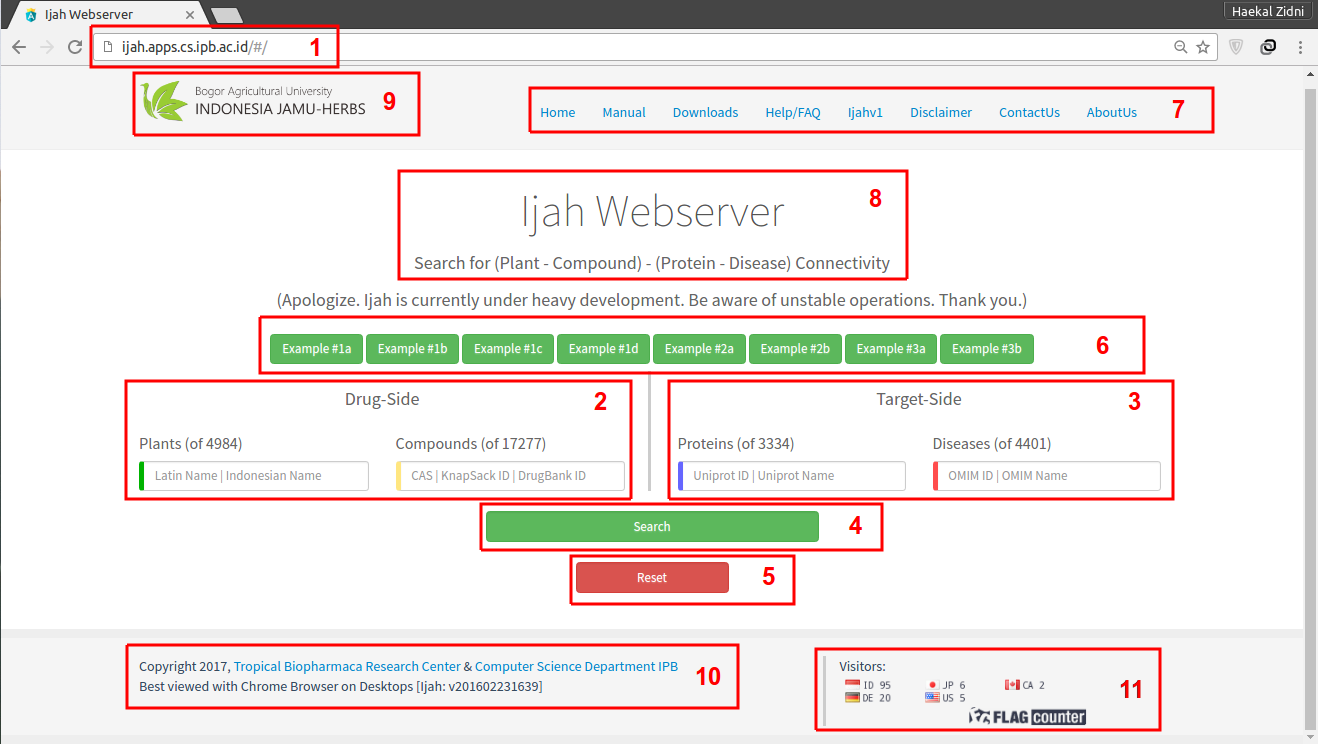
\includegraphics[scale=0.3]{ijah_home_overview.png}
		\caption{Halaman utama Ijah Webserver:
		(1) \hyperref[ssec:URL ijah]{URL Ijah};
		(2) \hyperref[sssec:drug input]{Kotak Masukan \emph{Drug-side}};
		(3) \hyperref[sssec:target input]{Kotak Masukan \emph{Target-side}};
		(4) \hyperref[sssec:search]{Tombol Eksekusi (Search/Search and Predict)};
		(5) \hyperref[sssec:reset]{Tombol Reset};
		(6) \hyperref[ssec:example button]{Deretan Tombol Contoh};
		(7) \hyperref[ssec:menu list]{Deretan Menu};
		(8) \hyperref[ssec:judul]{Judul};
		(9) \hyperref[ssec:judul]{Logo Ijah Webserver};
		(10) \hyperref[ssec:judul]{\emph{Copyright} dan versi Ijah};
		(11) \hyperref[ssec:visitor log]{\emph{Visitor Log}}}
		\label{fig:ijah_home_overview}
		\end{figure}

	\subsection{Kotak Masukan \emph{(Input Fields)}}
		\subsubsection{Drug-side} \label{sssec:drug input}
		Pada Drug-side, input terdiri dari tanaman (Plant) dan senyawa (Compound). Untuk menjaga konsistensi, ketika salah satu dipilih, maka pilihan lain akan menghilang, misal kita telah memilih untuk menginputkan Plant, maka Compound tidak bisa dipilih, begitu pula sebaliknya. Jika ingin mengembalikan/mengosongkan kondisi input kembali, gunakan tombol \hyperref[reset]{\textbf{Reset}}.
			\paragraph{Plants}
			Input Plant terdiri dari nama Latin dan nama Indonesia dari tanaman, yang dipisahkan oleh suatu garis vertikal. Hal ini memudahkan jika kita hanya mengetahui nama latin suatu tanaman dan tidak mengetahui nama lokalnya, begitu pula sebaliknya jika hanya mengetahui nama lokalnya. Selain membantu pencarian, pada kasus salah satu nama tidak diketahui maka akan didapat pengetahuan mengenai nama tanaman tersebut.
			\paragraph{Compounds}
			Input Compound terdiri dari ID CAS, \hyperref[knapsack]{ID KNApSAcK}, atau \hyperref[drugbank]{ID DrugBank} dari senyawa tersebut, setiap ID dipisahkan oleh garis vertikal. 
		\subsubsection{Target-side} \label{sssec:target input}
		Pada Target-side, input terdiri dari Protein dan penyakit (Disease). Untuk menjaga konsistensi, ketika salah satu dipilih, maka pilihan lain akan menghilang, misal kita telah memilih untuk menginputkan Protein, maka Disease tidak bisa dipilih, begitu pula sebaliknya. Jika ingin mengembalikan/mengosongkan kondisi input kembali, gunakan tombol \hyperref[reset]{\textbf{Reset}}.
			\paragraph{Protein}
			Input Protein terdiri dari \hyperref[uniprot]{nama Uniprot atau ID Uniprot}. Nama dan ID dipisahkan oleh garis vertikal.
			\paragraph{Disease}
			Input Disease terdiri dari \hyperref[omim]{nama OMIM atau ID OMIM}. Nama dan ID dipisahkan oleh garis vertikal.

	\subsection{Tombol Eksekusi}
	Setelah memberikan input, ada beberapa aksi yang dapat dilakukan, yaitu meneruskan pencarian dengan tombol Search atau mengosongkan semua input dengan tombol Reset.
		\subsubsection{Search (Search and Predict)} \label{sssec:search}
		Bergantung pada jenis input yang diberikan, tombol ini dapat menjalankan fungsi Search saja atau Search and Predict. Lengkapnya lihat pada bagian \hyperref[process]{\textbf{Proses}}.
		\subsubsection{Reset} \label{sssec:reset}
		Tombol Reset ini \textbf{memiliki fungsi yang cukup penting}. Saat ini terdapat kekurangan dimana saat menghapus input, input tidak benar-benar terhapus namun telah tersimpan untuk diproses. Sementara kekurangan ini masih diusahakan untuk diatasi, \textbf{\emph{sangat dianjurkan}} menggunakan tombol Reset ini untuk menghapus input ke kondisi kosong semula.

	\subsection{Deretan Tombol Contoh \emph{(Example)}} \label{ssec:example button}
	Deretan tombol contoh ini merupakan kumpulan contoh \emph{use-case} yang ada pada Ijah Webserver. Jadi selain menggunakan input manual, tombol-tombol contoh ini dapat memudahkan dalam menuju \emph{use-case} tertentu. Kumpulan contoh ini terbagi menjadi tiga kelompok, dimana Example \#1a - \#1d merupakan \emph{use-case} \hyperref[end to end]{\emph{Both Drug and Target inputs}}, Example \#2a - \#2b merupakan \emph{use-case} \hyperref[drug only]{\emph{Drug inputs only}}, dan Example \#3a - \#3b merupakan \emph{use-case} \hyperref[target only]{\emph{Target inputs only}}. Lebih lengkapnya:

	\begin{itemize}
	\item \textbf{Example \#1a} - Plant-Disease
	\item \textbf{Example \#1b} - Plant-Protein
	\item \textbf{Example \#1c} - Compound-Protein
	\item \textbf{Example \#1d} - Compound-Disease
	\item \textbf{Example \#2a} - Plant search only
	\item \textbf{Example \#2b} - Compound search only
	\item \textbf{Example \#3a} - Protein search only
	\item \textbf{Example \#3b} - Disease search only
	\end{itemize}

	\subsection{Deretan Menu} \label{ssec:menu list}
	Pada bagian ini ada sederetan menu yang dapat di-klik. Penjelasan lebih lanjut tentang menu ini ada pada bagian \textbf{\nameref{Menu}}.

	\subsection{Judul, Versi, Logo, dan \emph{Copyright} Ijah} \label{ssec:judul}
	Pada bagian tengah halaman terdapat judul webserver ini, yaitu \textbf{``Ijah Webserver -- Search for (Plant-Compound) -- (Protein-Disease) Connectivity''}. Logo Ijah terdapat pada bagian kiri atas. Pada bagian bawah kiri halaman terdapat bagian yang berisi \emph{copyright} dan versi Ijah Webserver yang berjalan. Di bagian ini juga ada saran penggunaan untuk pengalaman terbaik saat menggunakan Ijah Webserver. Pada nomor versi Ijah Webserver, 8 digit pertama merupakan format tahun-bulan-tanggal dan 4 digit terakhir merupakan jam dan menit. Sebagai contoh di Ijah Webserver v201702231639 berarti versi ini di-\emph{deploy} pada tanggal 23 Februari 2017 pukul 16:39. Pada \emph{copyright} dijelaskan bahwa hak cipta Ijah Webserver ada pada Departemen Ilmu Komputer IPB dan Pusat Riset Biofarmaka IPB.


	\subsection{Visitor Log} \label{ssec:visitor log}
	Visitor Log terdapat di sebelah kanan bawah, setelah \emph{copyright} dan versi. Visitor Log adalah fitur yang menghitung jumlah kunjungan Ijah Webserver beserta negara asal kunjungan. Area Visitor Log ini dapat diklik untuk melihat statistik kunjungan lebih lengkap, seperti pada gambar \ref{fig:ijah_flagcount}

	\begin{figure}[H]
	\centering
	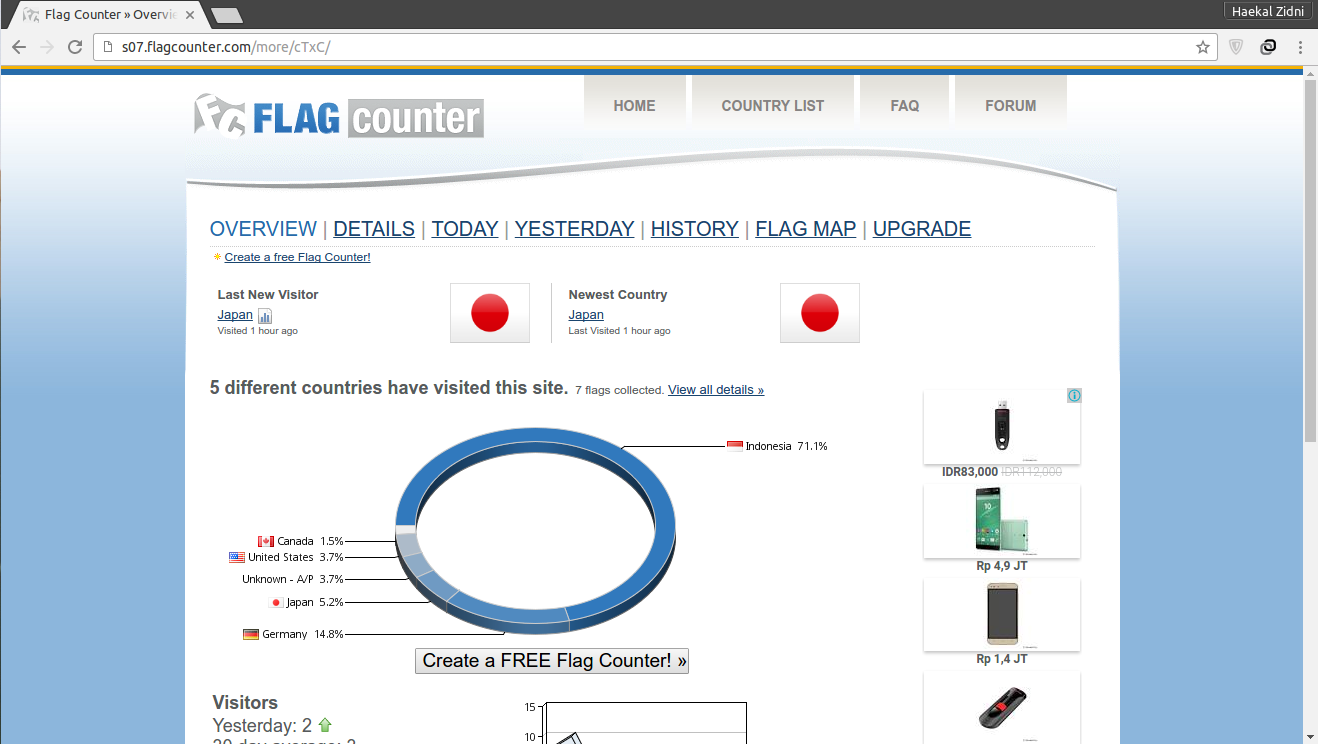
\includegraphics[scale=0.3]{ijah_flagcount.png}
	\caption{Statistik lebih detail yang akan muncul setelah mengklik area Visitor Log}
	\label{fig:ijah_flagcount}
	\end{figure}

\section{Repositori \emph{Source Code}} \label{sec:ws_source}
\emph{Source Code} untuk Ijah Webserver dapat diakses di repositori GitHub di alamat URL \href{https://github.com/tttor/csipb-jamu-prj}{\textbf{https://github.com/tttor/csipb-jamu-prj}}.

Pada repositori ini terdapat beberapa folder untuk setiap \emph{source code}

\begin{itemize}
\item \textbf{Webserver}\\
\href{https://github.com/tttor/csipb-jamu-prj/tree/master/webserver}{\textbf{https://github.com/tttor/csipb-jamu-prj/tree/master/webserver}}.
\item \textbf{Predictor}\\
\href{https://github.com/tttor/csipb-jamu-prj/tree/master/predictor}{\textbf{https://github.com/tttor/csipb-jamu-prj/tree/master/predictor}}.
\item \textbf{Database} (lihat bab \ref{db chapter} )\\
\href{https://github.com/tttor/csipb-jamu-prj/tree/master/database}{\textbf{https://github.com/tttor/csipb-jamu-prj/tree/master/database}}.
\end{itemize}

%% This is an example first chapter.  You should put chapter/appendix that you
%% write into a separate file, and add a line \include{yourfilename} to
%% main.tex, where `yourfilename.tex' is the name of the chapter/appendix file.
%% You can process specific files by typing their names in at the 
%% \files=
%% prompt when you run the file main.tex through LaTeX.
%\chapter{Use Case 1 - Both Drug and Target Side} \label{Use Case}
\chapter{Langkah-langkah Penggunaan}
Pada bagian ini akan dijelaskan secara rinci langkah-langkah penggunaan Ijah Webserver. Langkah-langkah ini mengacu pada Use-case 1 (Plant-Disease). Untuk use-case lainnya mirip, hanya berbeda pada masukan yang diisikan.

\section{Memberikan Masukan \emph{(inputs)}}

\begin{figure}[H]
	\centering
	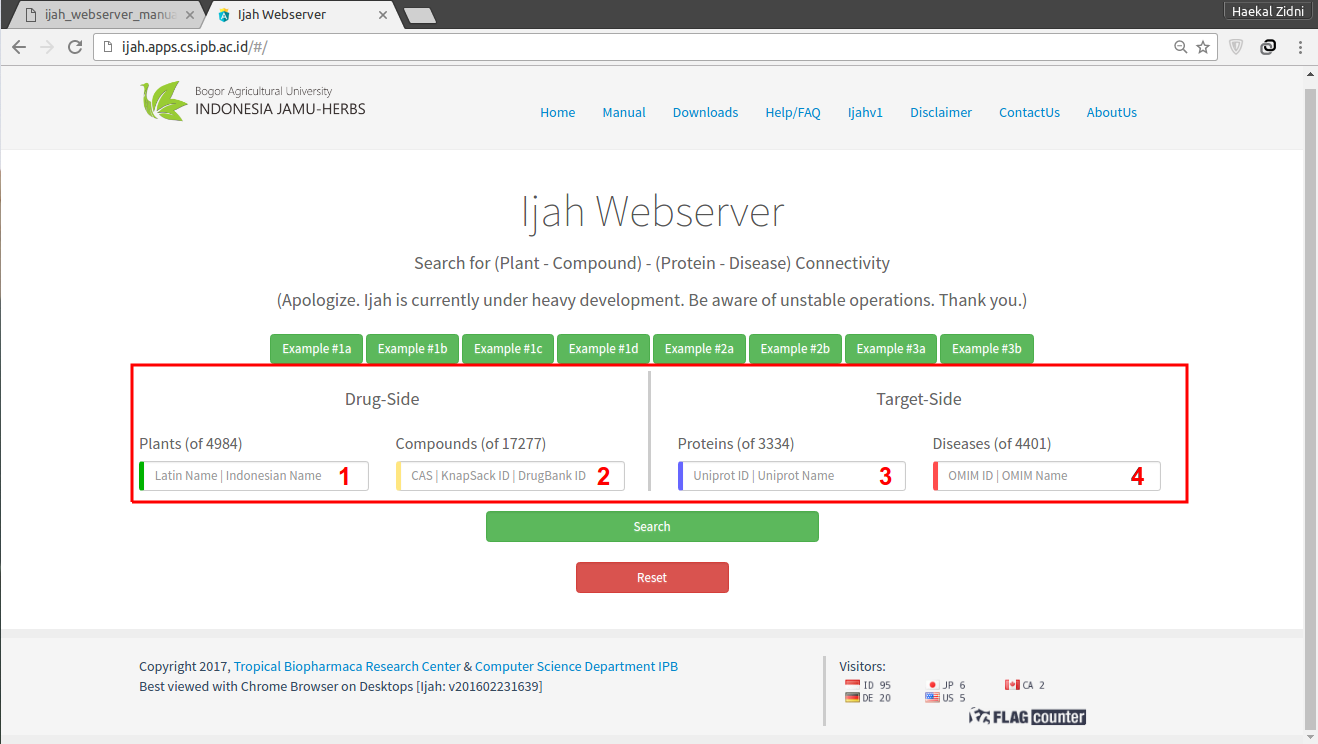
\includegraphics[scale=0.3]{ijah_input_form.png}
	\caption{Input Fields Ijah Webserver: Drug-Side - (1) Plants, (2) Compounds, Target-side - (3) Proteins, (4) Diseases}
	\label{fig:ijah_input_form}
	\end{figure}

	\subsection{Drug-side input}
	Pada saat memberikan masukan pada \emph(input fields) Ijah, perlu diperhatikan bahwa Ijah Webserver telah memiliki fitur \emph{autocomplete}, cukup mengetikkan sebagian dari nama latin atau nama Indonesia pada Plants atau salah satu ID dari input lainnya, maka saran yang mendekati hasil yang dimaksud sudah muncul. Untuk memulai, masukkan input pada Drug-side, misal tanaman.

	\begin{figure}[H]
		\centering
		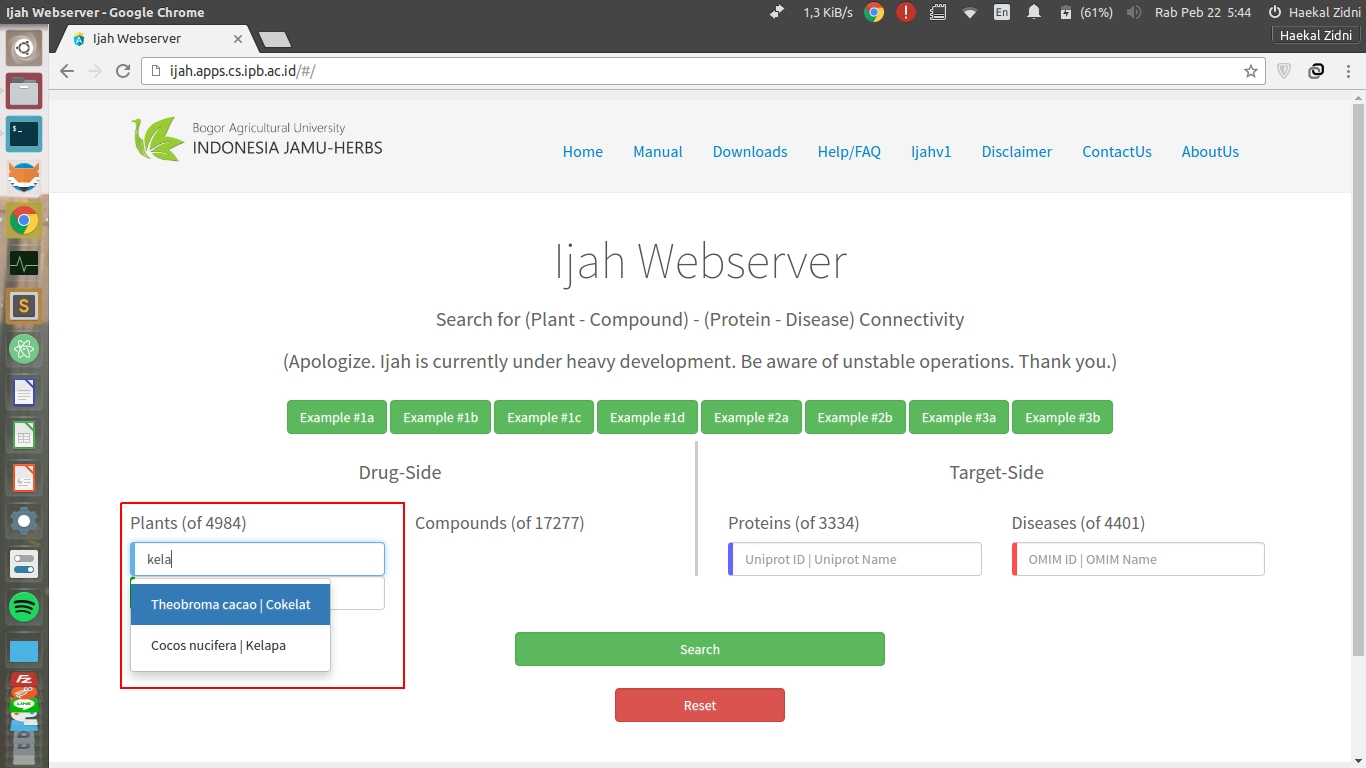
\includegraphics[scale=0.3]{ijah_autocomplete.png}
		\caption{Contoh saran dari \emph{autocomplete} ketika memasukkan `lida'}
		\label{fig:ijah_autocomplete_click}
		\end{figure}

	Untuk memilih, klik pilihan yang diinginkan. \textbf{Penting:} mengetikkan input secara manual hingga akhir tidak akan dianggap sebagai input yang \emph{valid}. Klik pilihan yang diinginkan agar masuk sebagai input yang\emph{valid}.

	Sebagai contoh, kita ingin memasukkan lidah buaya. Klik \mbox{\textbf{``Aloe Vera | Lidah Buaya''}} pada pilihan yang muncul. Jika sudah diklik, maka kotak akan terisi.

	\begin{figure}[H]
		\centering
		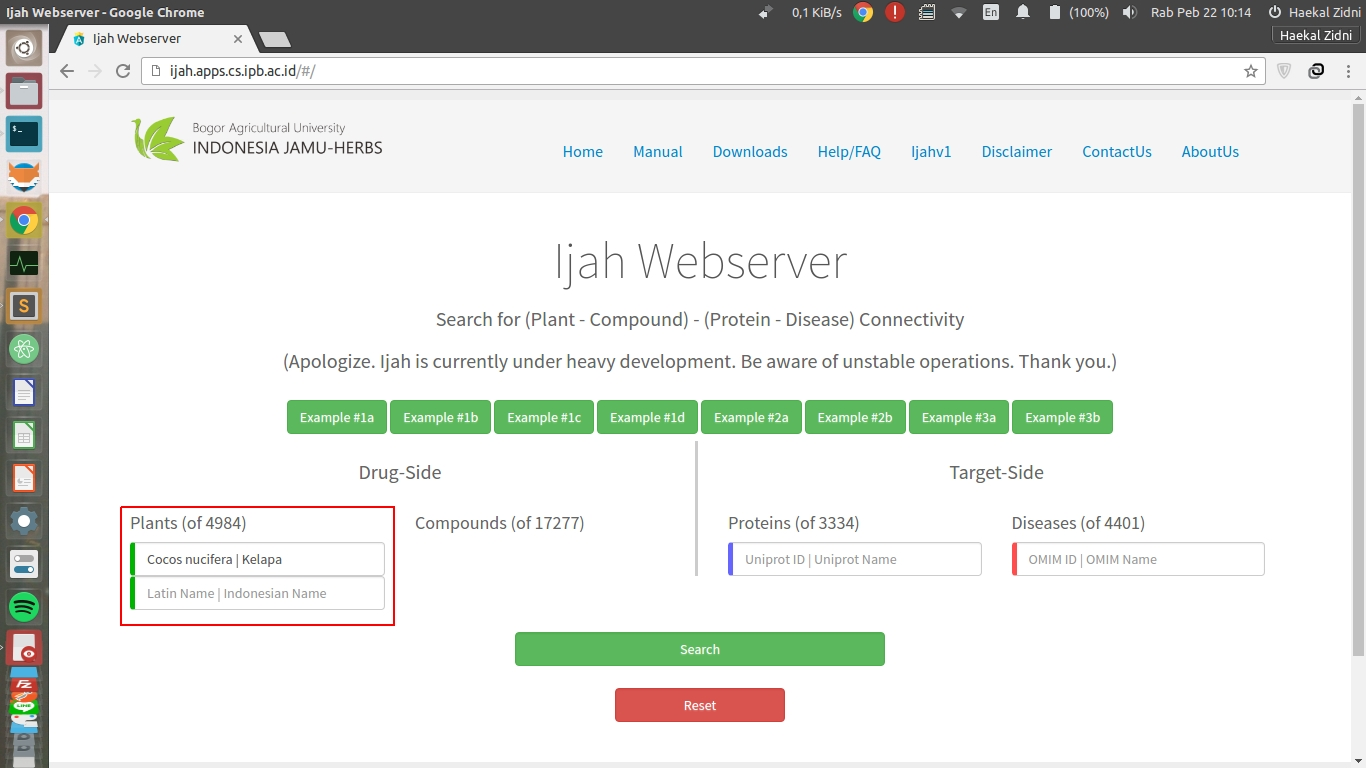
\includegraphics[scale=0.3]{ijah_autocomplete_complete.png}
		\caption{Setelah diklik input akan terlengkapi, dan kotak baru muncul di bawahnya}
		\label{fig:ijah_autocomplete_complete}
		\end{figure}

	Setelah memasukkan satu input, maka kotak baru akan muncul secara otomatis, jika kita ingin menambahkan input di kategori itu. Kotak baru akan terus muncul setelah satu input yang \emph{valid} masuk. Langkah ini berlaku untuk \emph{field} lain seperti Compounds, Proteins, dan Diseases.

	Perlu diperhatikan, pada gambar \ref{fig:ijah_autocomplete_complete}, saat input hanya berasal dari satu Side (dalam kasus ini hanya pada Drug-side), tombol eksekusi akan berlabelkan \textbf{Search} saja. Jika input terisi dari kedua Side maka label tombol akan berubah seperti pada gambar \ref{fig:ijah_autocomplete_complete2}.

	\subsection{Target-side input}
	Setelah memasukkan input dari Drug-side (dalam use-case ini memasukkan tanaman), maka dilanjutkan dengan memasukkan input dari Target-side. Cara memberikan masukan tetap sama. Kali ini sebagai contoh akan diinputkan disease \mbox{\textbf{``614292 | Myopia, high, with cataract and vitreoretinaldegeneration''}}

	\begin{figure}[H]
		\centering
		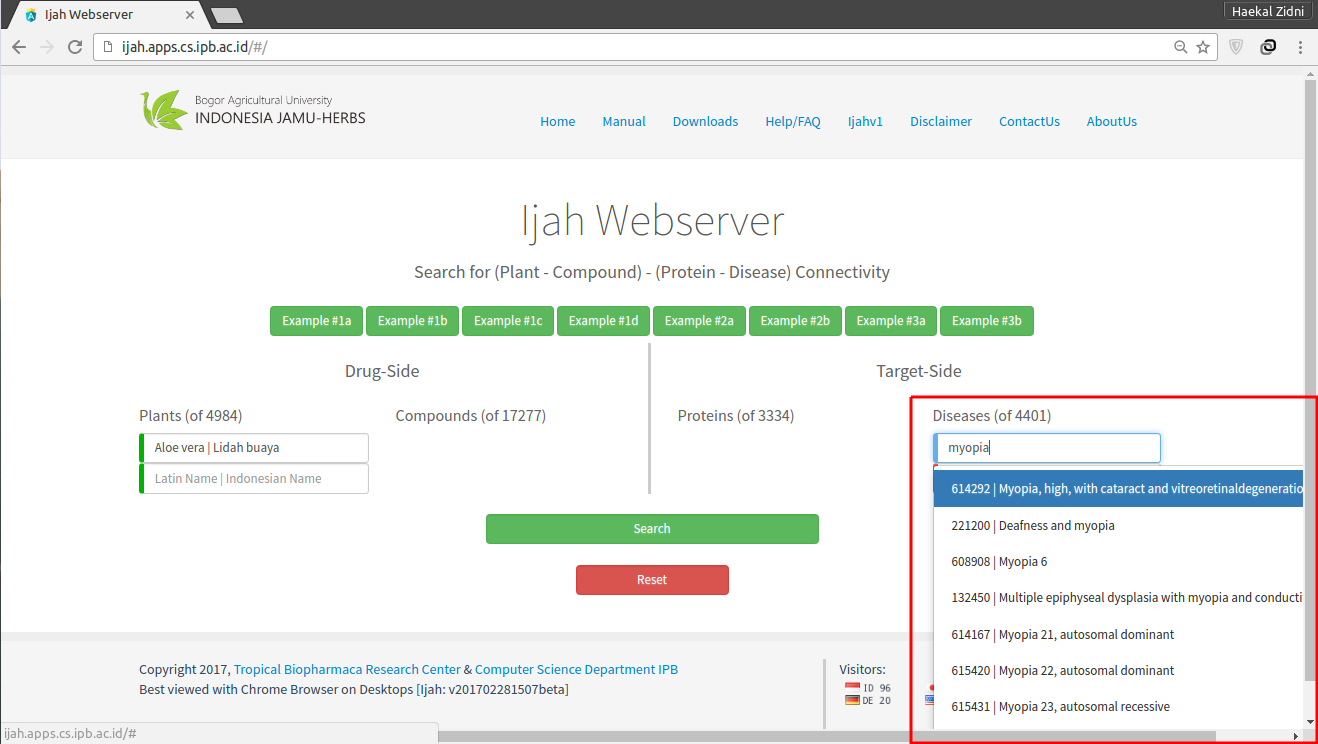
\includegraphics[scale=0.3]{ijah_autocomplete2.png}
		\caption{\emph{autocomplete} pada saat memasukkan Target berupa Disease}
		\label{fig:ijah_autocomplete_click2}
		\end{figure}

	\begin{figure}[H]
		\centering
		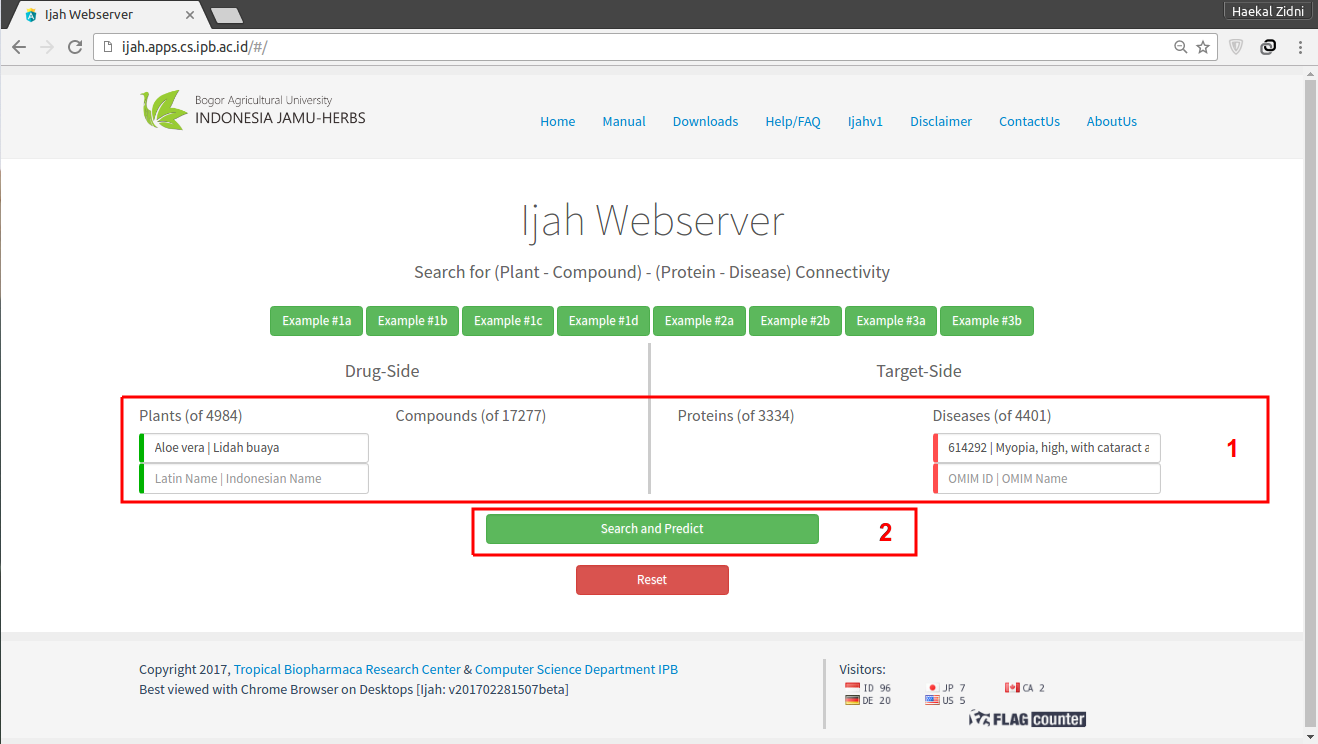
\includegraphics[scale=0.3]{ijah_autocomplete_complete2.png}
		\caption{(1) Input dari kedua sisi sudah lengkap. (2) Perhatikan tombol eksekusi yang berlabel \emph{textbf{Search and Predict}}}
		\label{fig:ijah_autocomplete_complete2}
		\end{figure}


\section{Memproses Input} \label{process}
Setelah memasukkan input, langkah berikutnya yaitu input dapat diproses. Setelah tombol eksekusi diklik, maka proses Search and Predict akan berjalan. Selama proses berjalan, akan muncul animasi seperti pada gambar \ref{fig:ijah_process_bounce}

\begin{figure}[H]
	\centering
	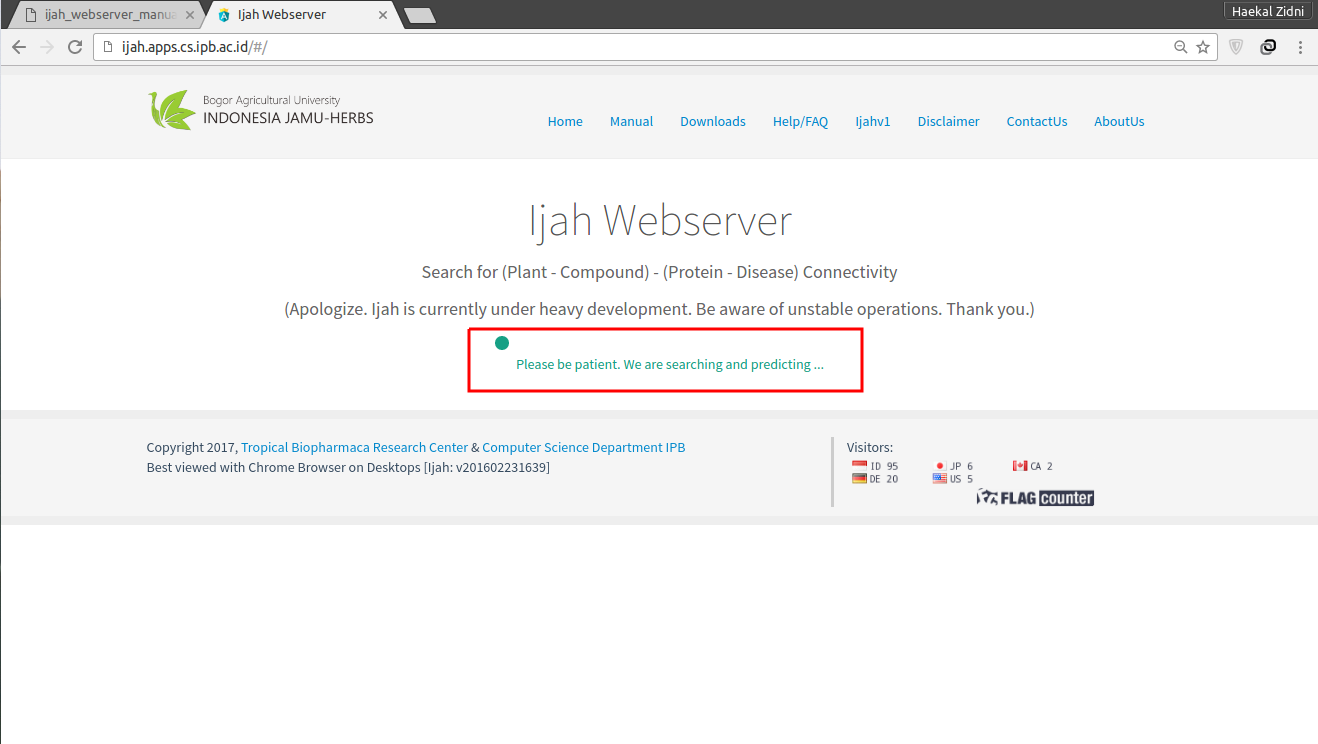
\includegraphics[scale=0.3]{ijah_process_bounce.png}
	\caption{Animasi saat proses Search and Predict sedang berlangsung}
	\label{fig:ijah_process_bounce}
	\end{figure}

\section{Membaca luaran \emph{(outputs)}}
\textbf{Catatan:} jika layout halaman output terlihat saling menumpuk, silakan \emph{zoom out} browser anda hingga terlihat sesuai (bergantung resolusi monitor anda).

Setelah proses selesai, maka luaran \emph{(output)} yang dihasilkan sudah dapat dibaca. Terdapat empat kategori \emph{output} yang dihasilkan, yaitu:
	
	\subsection{Summary} \label{summary}
	\begin{figure}[H]
	\centering
	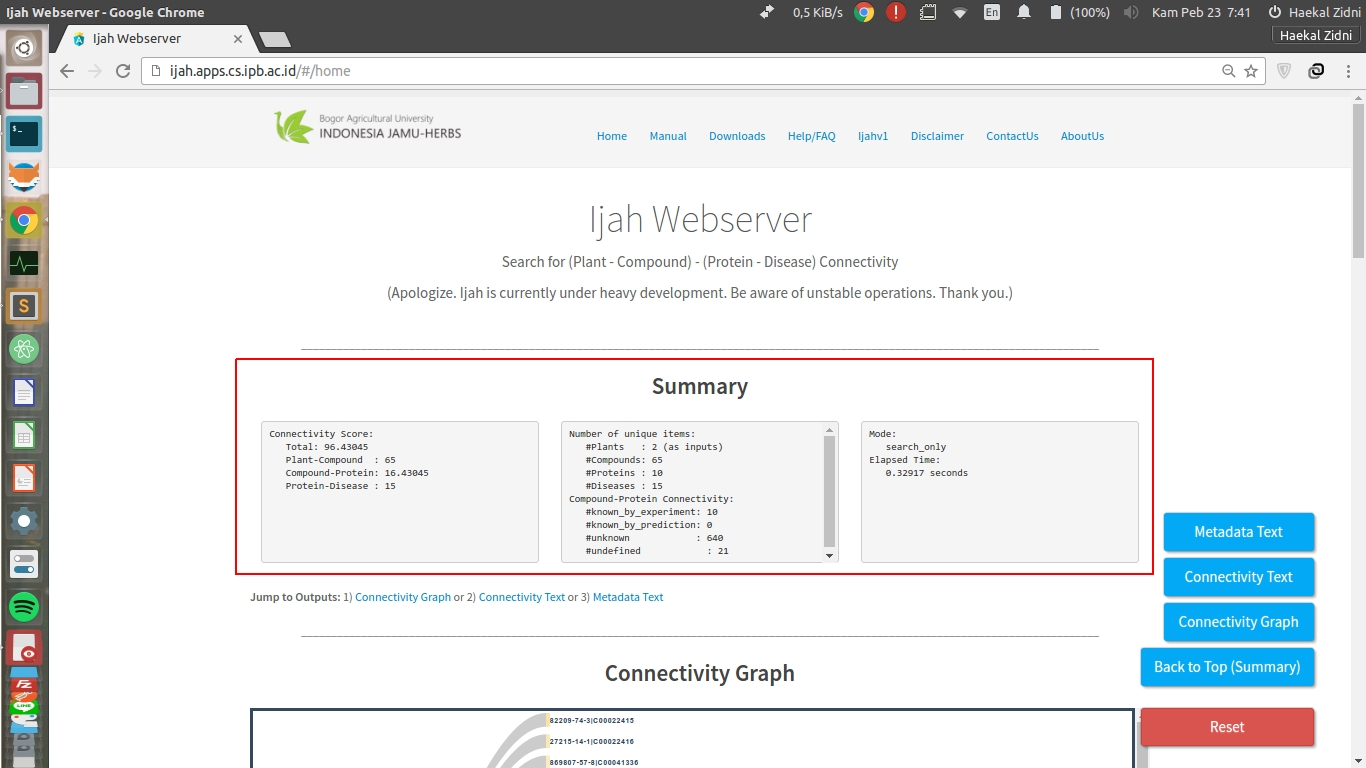
\includegraphics[scale=0.3]{ijah_output_summary.png}
	\caption{Output Summary}
	\label{fig:ijah_output_summary}
	\end{figure}
	
	Output Summary adalah ringkasan dari proses output, yang meliputi:
	\begin{enumerate}
	\item \textbf{Minimum Connectivity Weight to Process} -- nilai minimum skor yang diproses, dapat diubah melalui filter yang akan dijelaskan di bagian \hyperref[nav]{Filter pada Navigasi}.
	\item \textbf{Connectivity Score} -- jumlah total dari nilai seluruh konektivitas (1 artinya 100\% terhubung, 0 tidak terhubung, di antara 1 dan 0 berarti hasil prediksi yang nilainya belum 100\%, seluruh keterhubungan dijumlah untuk mendapat nilai total).
	\item \textbf{Number of Unique Items} -- jumlah entitas unik (tidak termasuk pengulangan) yang terlibat dalam proses.
	\item \textbf{Compound-Protein Connectivity} -- jumlah konektivitas senyawa dan protein. \textbf{Known by experiment} artinya data sudah valid 100\%, berasal dari pangkalan data, sedangkan \textbf{Known by prediction} berarti konektivitas hasil prediksi algoritme, \textbf{Unknown} artinya konektivitas yang tidak diketahui baik dari pangkalan data maupun hasil prediksi algoritme.
	\item \textbf{Mode} -- mode proses, apakah Search saja atau Search and Predict.
	\item \textbf{Elapsed Time} -- waktu yang dihabiskan untuk menyelesaikan proses.
	\end{enumerate}
	
	\subsection{Connectivity Graph} \label{graph}
	Connectivity Graph merupakan model output yang berupa \emph{multi-partite graph}, yaitu graf yang verteksnya terbagi menjadi beberapa partisi.

	\begin{figure}[H]
	\centering
	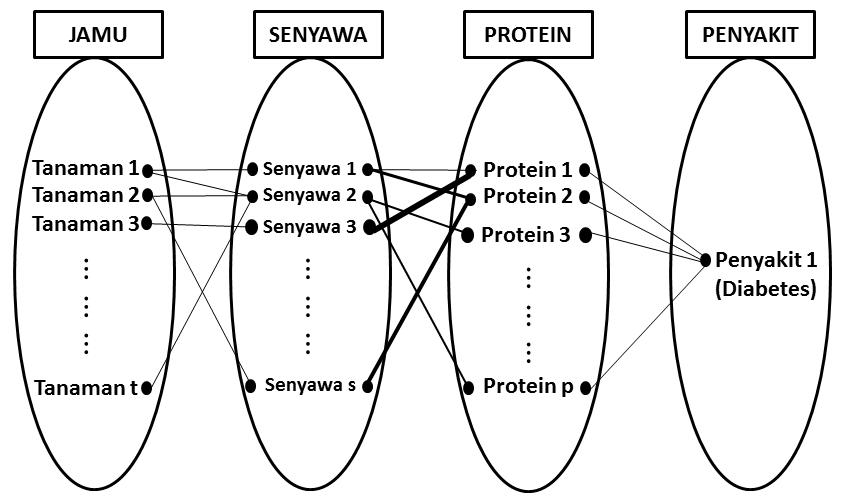
\includegraphics[scale=0.5]{multipartite-graph.png}
	\caption{Contoh \emph{multipartite graph}}
	\label{fig:multipartite-graph}
	\end{figure}

	\begin{figure}[H]
	\centering
	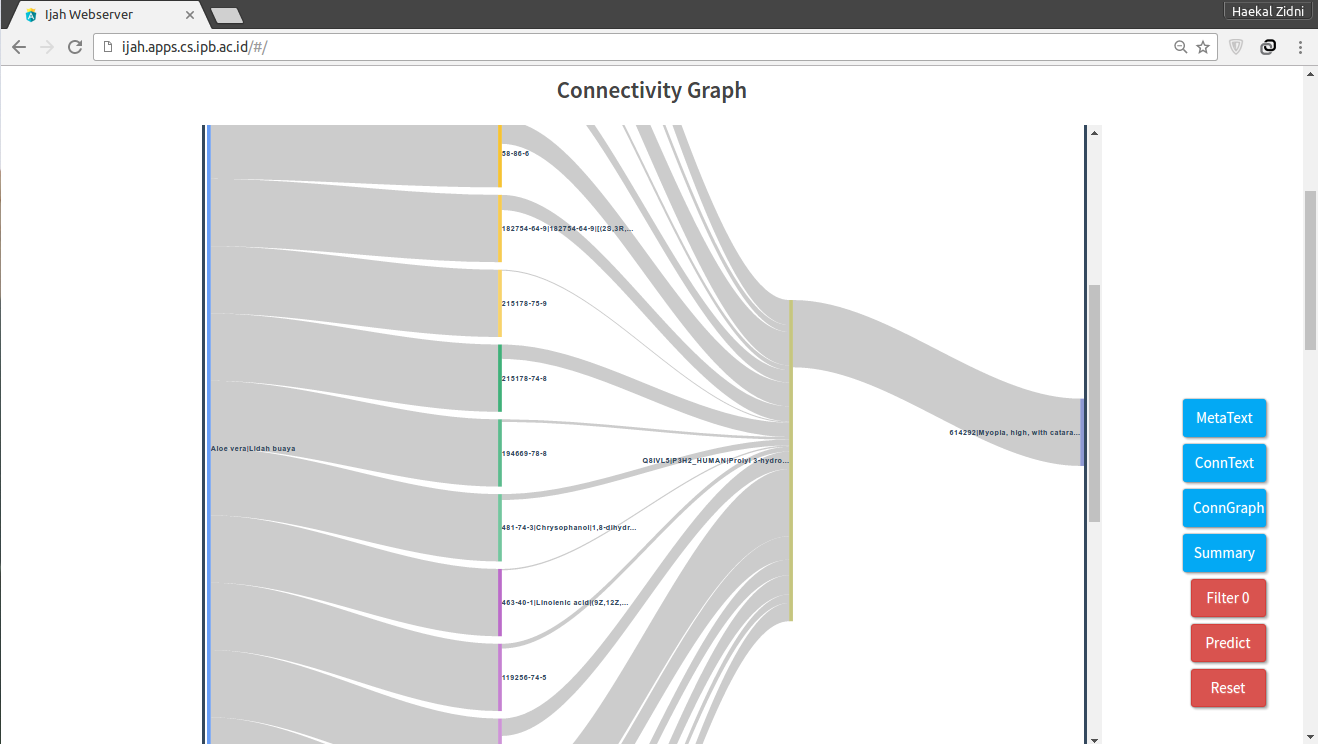
\includegraphics[scale=0.3]{ijah_output_graph.png}
	\caption{Connectivity Graph pada Ijah Webserver}
	\label{fig:ijah_output_graph}
	\end{figure}
	
	Pada model Connectivity Graph Output, terdapat vertex dari Plant ke Compound, Compound ke Protein, dan Protein ke Disease, ada 4 partisi pada graf ini.

	\begin{figure}[H]
	\centering
	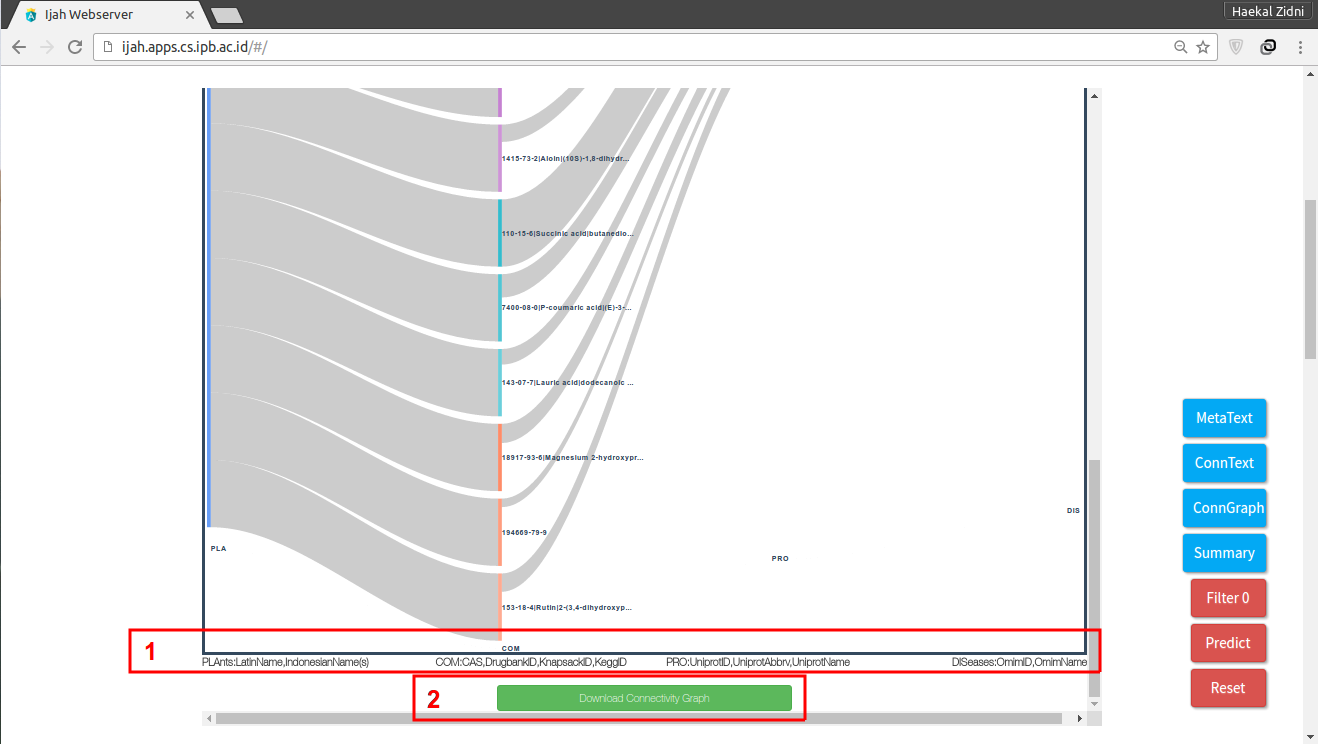
\includegraphics[scale=0.3]{ijah_output_graph_bottom.png}
	\caption{Bagian bawah Connectivity Graph -- (1) Keterangan Graf, (2) Tombol Download}
	\label{fig:ijah_output_graph_bottom}
	\end{figure}

	Pada bagian bawah dan atas graf terdapat panduan setiap partisi graf, dari paling kiri Plants (nama latin | nama Indonesia), lalu Compounds (dan IDnya (CAS, Drugbank, Knapsack, Kegg)), Proteins dan IDnya (nama Uniprot, singkatan (abbrv) Uniprot, ID Uniprot), dan Diseases beserta IDnya di paling kanan (ID dan nama OMIM).

	Navigasi graf dapat dilakukan dengan menggulir \emph{scrolling} ke atas dan bawah. Graf ini bisa didownload menggunakan tombol Download di bawah graf, dengan format gambar PNG.
	
	\subsection{Connectivity Text} \label{text}

	Selain dalam bentuk \emph{multipartite graph}, output juga dihasilkan dalam bentuk Connectivity Text, yaitu teks yang berisi konektivitas antar entitas

	\begin{figure}[H]
	\centering
	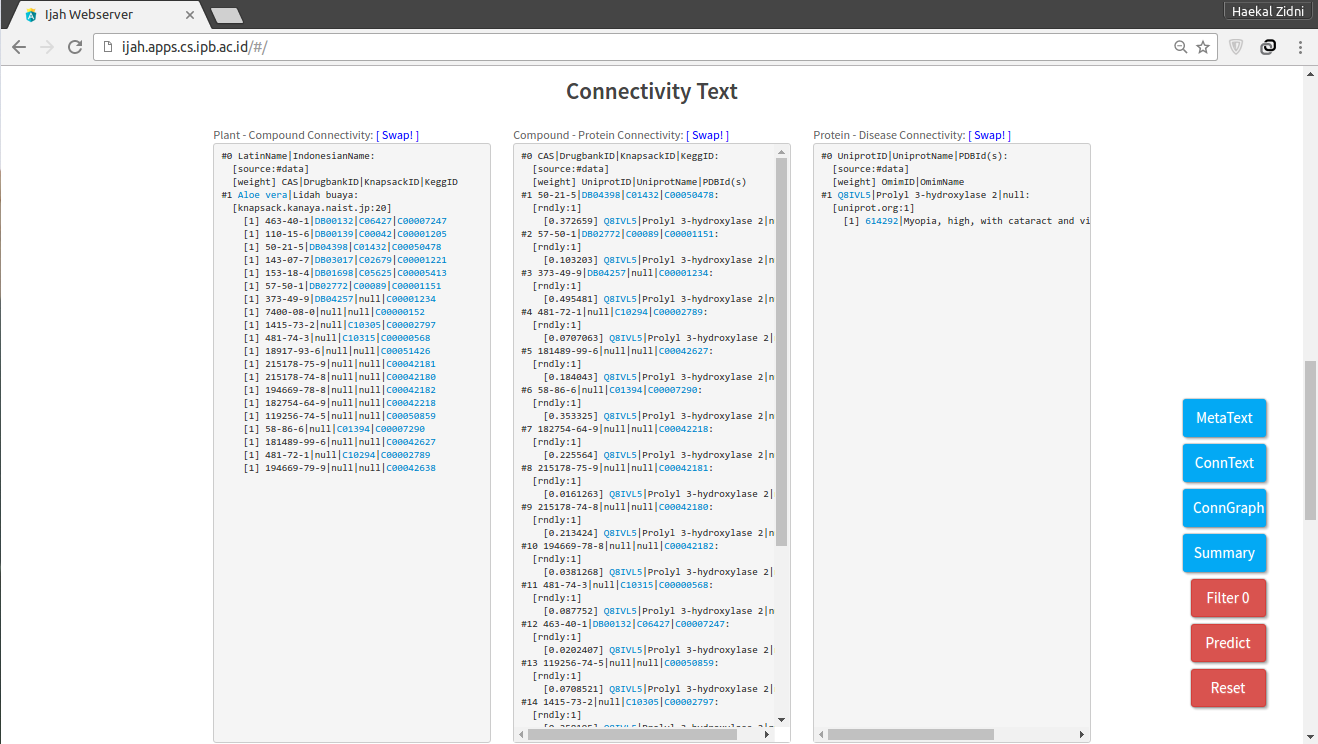
\includegraphics[scale=0.3]{ijah_output_text.png}
	\caption{Connectivity Text pada Ijah Webserver}
	\label{fig:ijah_output_text}
	\end{figure}	
	
	Isi pada output Text yaitu data konektivitas (nama dan ID entitas pertama), sumber data konektivitas, serta bobot nilai konektivitas (1 jika terhubung 100\% by experiment, jika by prediction nilainya akan bervariasi antara 0 sampai 1, lebih mendekati 1 maka lebih baik), lalu nama dan ID entitas keduanya.

	Pada output Text, dapat dilakukan \emph{swapping} konektivitas, misal dari Plant-Compound menjadi Compound-Plant. Hal ini dapat dilakukan dengan mengklik tombol \textbf{Swap!} di bagian atas tiap kotak konektivitas.

	\begin{figure}[H]
	\centering
	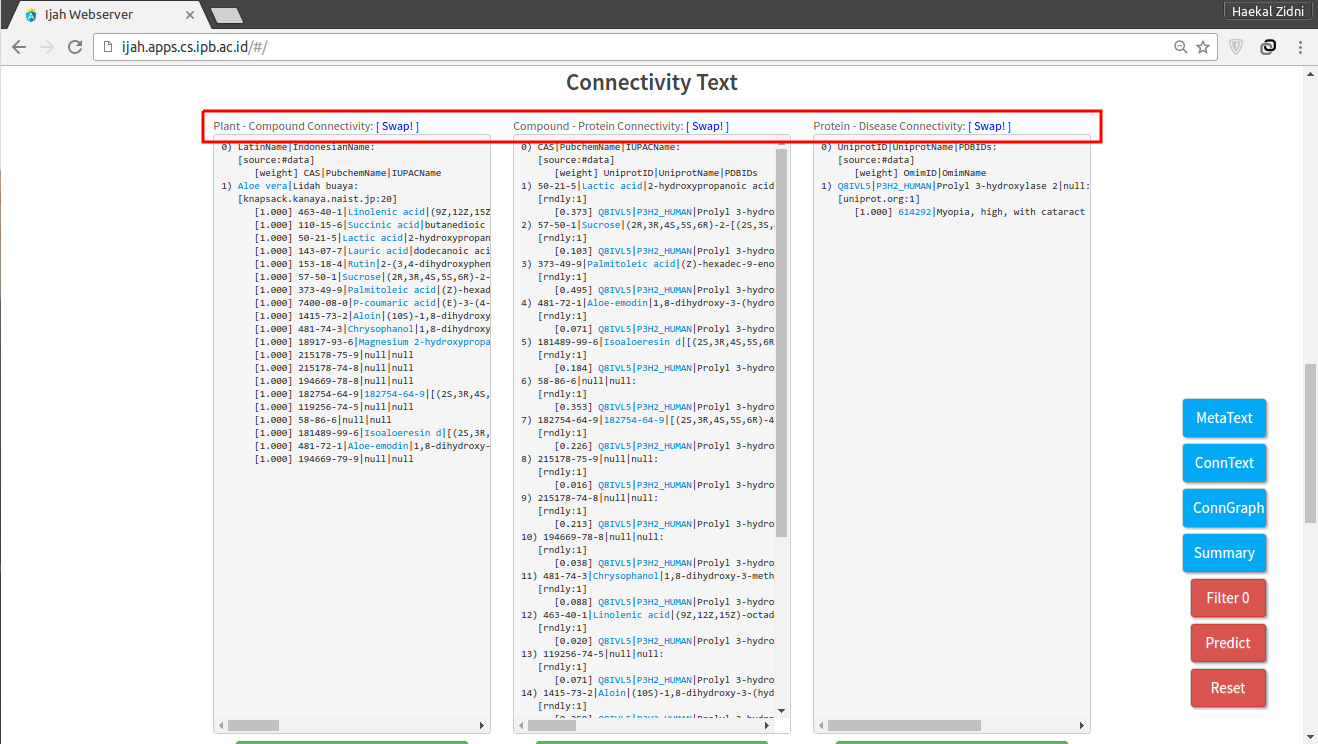
\includegraphics[scale=0.3]{ijah_output_text_swapbutton.png}
	\caption{Posisi tombol Swap untuk Connectivity Text}
	\label{fig:ijah_output_text_swapbutton}
	\end{figure}

	\begin{figure}[H]
	\centering
	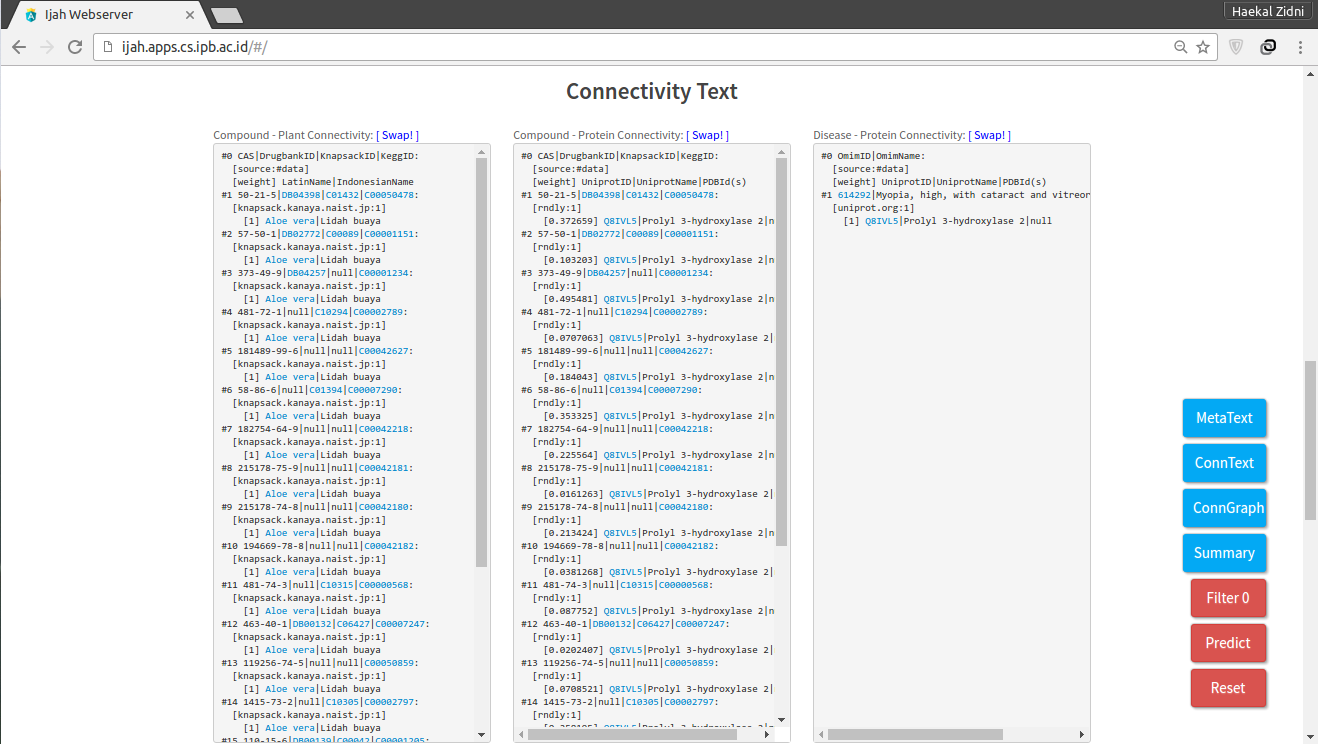
\includegraphics[scale=0.3]{ijah_output_text_swapped.png}
	\caption{Hasil Swapping pada Plant-Compound dan Protein-Disease. Perhatikan bahwa konektivitasnya berubah menjadi Compound-Plant dan Disease-Protein}
	\label{fig:ijah_output_text_swapped}
	\end{figure}

	Seperti Connectivity Graph, Connectivity Text juga memiliki tombol Download untuk mendownload file teks konektivitas ini. Download dilakukan per konektivitas sehingga terbagi menjadi tiga file.

	\begin{figure}[H]
	\centering
	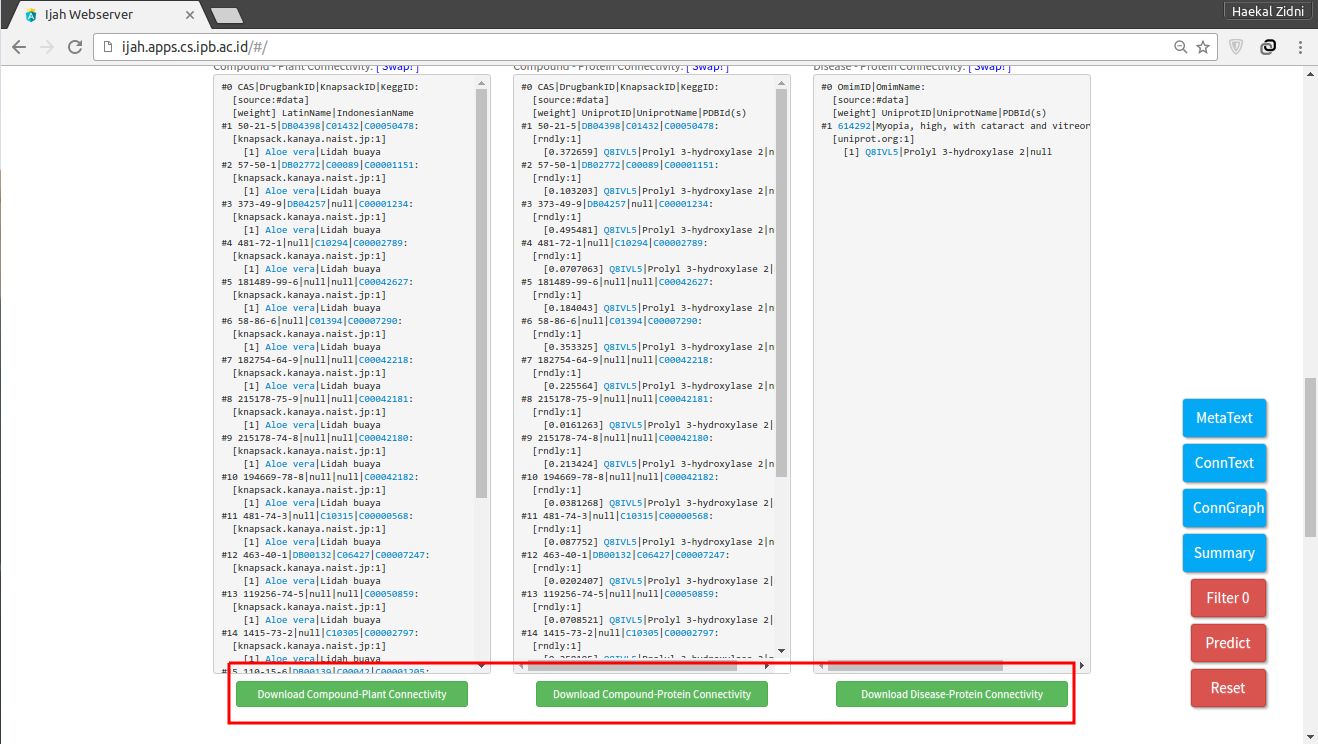
\includegraphics[scale=0.3]{ijah_output_text_download.png}
	\caption{Tombol Download untuk mengunduh file teks konektivitas}
	\label{fig:ijah_output_text_download}
	\end{figure}
	
	\subsection{Metadata Text} \label{meta}
	Metadata Text berisi metadata (nama dan ID) dari semua entitas yang terlibat dalam proses ini. Pada bagian bawah, juga terdapat tombol Download untuk mengunduh teks Metadata ini. Pada metadata ini, jika ada item yang tidak ditampilkan pada salah satu entitas namun ada di entitas lainnya, artinya \emph{value} item tersebut pada entitas tersebut tidak ada. Sebagai contoh, pada metadata Compounds, ada beberapa senyawa yang tidak memiliki nama PubChem sehingga tidak ditampilkan.

	\begin{figure}[H]
	\centering
	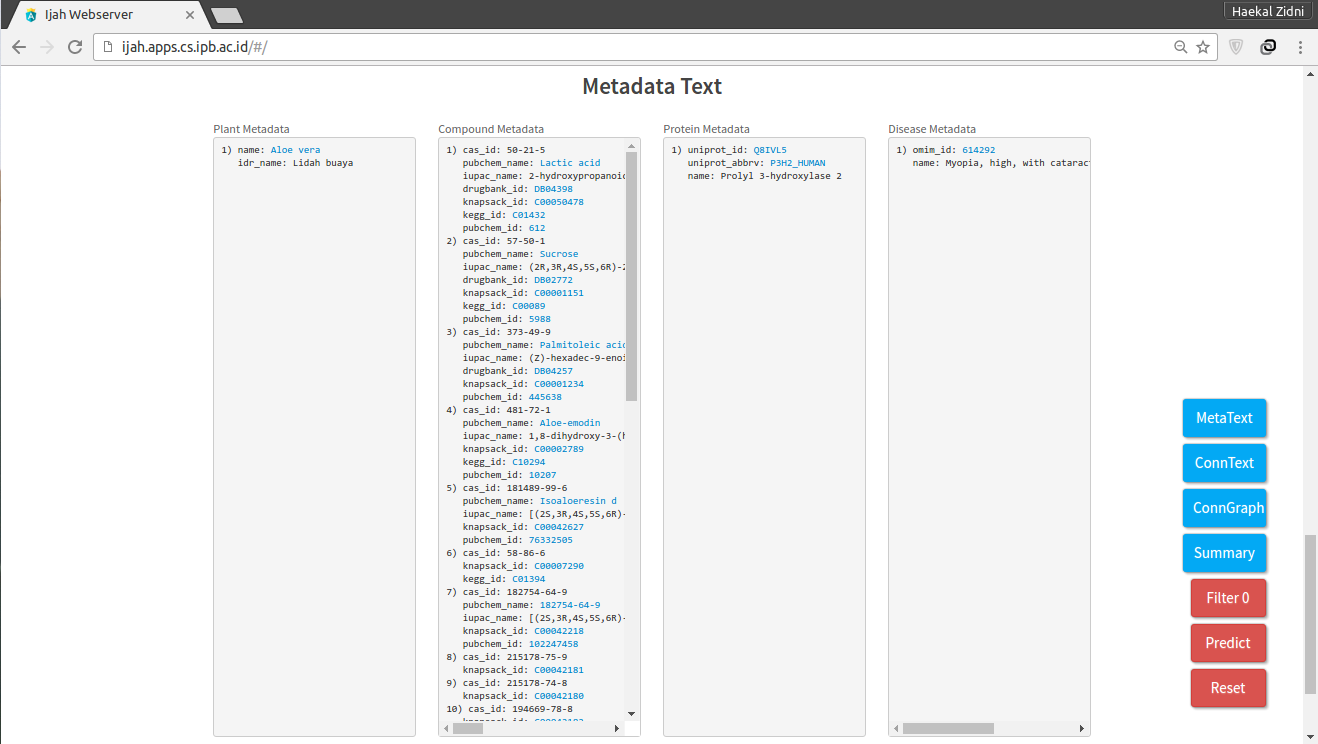
\includegraphics[scale=0.3]{ijah_output_meta.png}
	\caption{Metadata Text Output pada Ijah Webserver}
	\label{fig:ijah_output_meta}
	\end{figure}

	\begin{figure}[H]
	\centering
	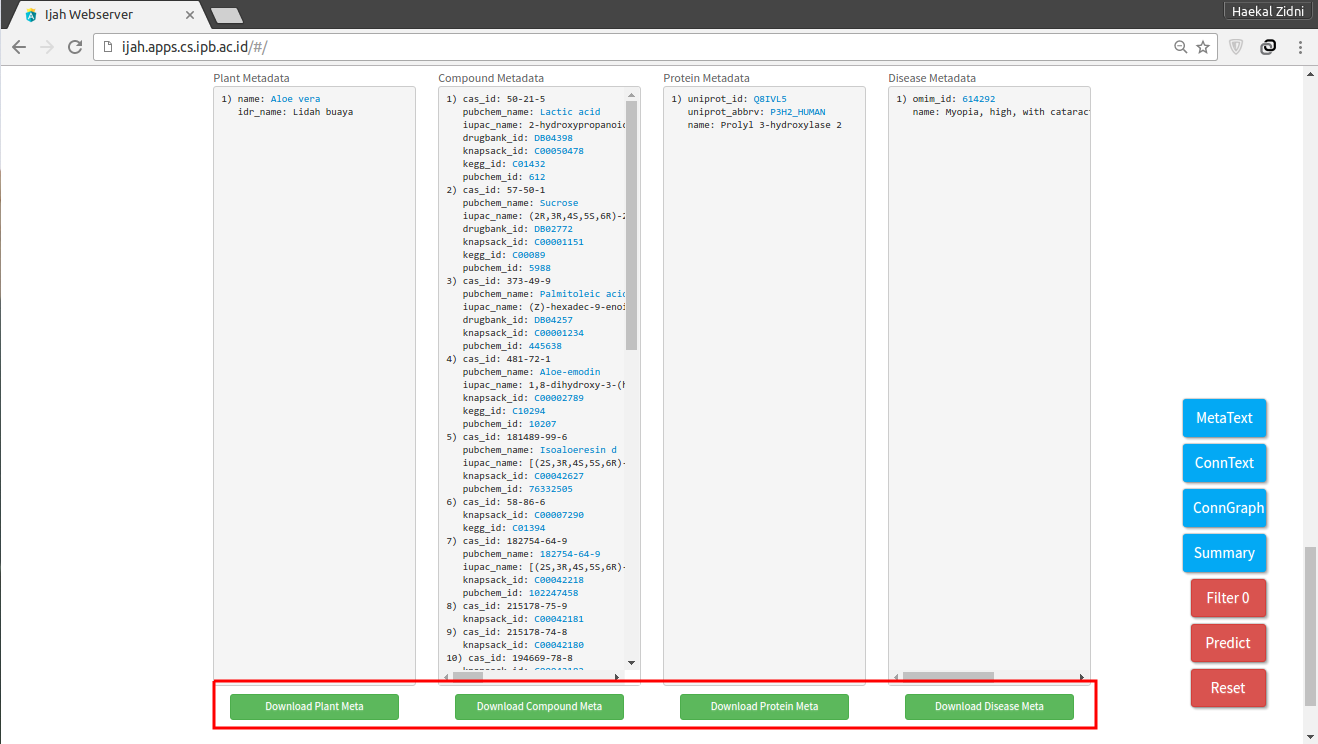
\includegraphics[scale=0.3]{ijah_output_meta_download.png}
	\caption{Tombol Download untuk mengunduh file teks Metadata}
	\label{fig:ijah_output_meta_download}
	\end{figure}


\section{Memodifikasi Output}
Pada halaman output, terdapat \emph{floating button} di sisi kanan bawah yang berisi beberapa fungsi.

	\begin{figure}[H]
	\centering
	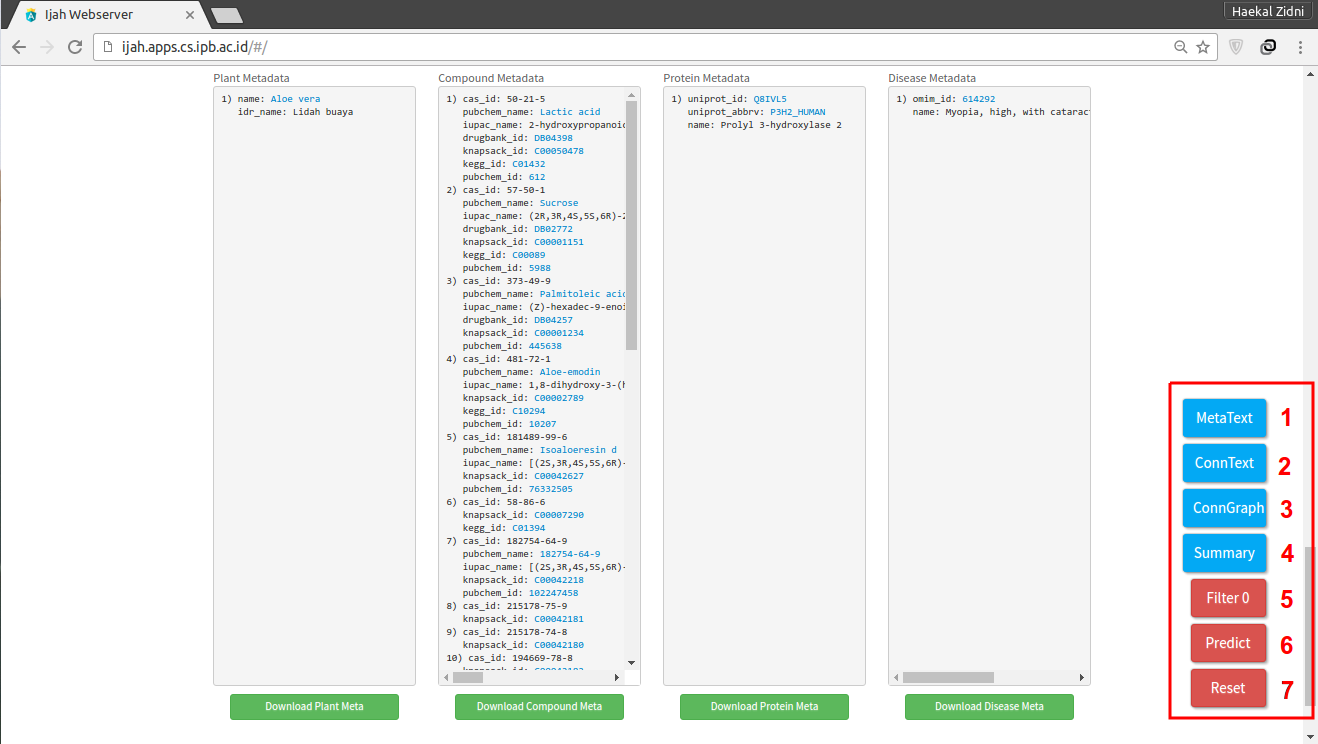
\includegraphics[scale=0.3]{ijah_floating.png}
	\caption{Floating button pada Ijah Webserver}
	\label{fig:ijah_floating}
	\end{figure}

Tombol-tombol pada \emph{floating button} beserta fungsinya:
\begin{enumerate}
\item \textbf{MetaText:} jalan pintas menuju \hyperref[meta]{\textbf{Metadata Text Output}}
\item \textbf{ConnText:} jalan pintas menuju \hyperref[text]{\textbf{Connectivity Text Output}}
\item \textbf{ConnGraph:} jalan pintas menuju \hyperref[graph]{\textbf{Connectivity Graph Output}}
\item \textbf{Summary:} jalan pintas menuju \hyperref[summary]{\textbf{Summary}}
\item \textbf{Filter:} akan dibahas pada bagian \hyperref[filter]{\textbf{Filter}}
\item \textbf{Predict:} akan dibahas pada bagian \hyperref[predictmore]{\textbf{Predict}}
\item \textbf{Reset:} mengosongkan seluruh hasil proses dan mengulang ke halaman awal.
\end{enumerate}

	\subsection{Filter} \label{filter}
	Tombol Filter berfungsi untuk menyaring skor konektivitas yang akan ditampilkan. Filter ini memiliki beberapa level yaitu:
	\begin{itemize}
	\item 0 - Menampilkan keseluruhan konektivitas yang ada (minimum skor 0).
	\item 0.2 - Menampilkan konektivitas dengan skor minimal 0.2
	\item 0.4 - Menampilkan konektivitas dengan skor minimal 0.4
	\item 0.6 - Menampilkan konektivitas dengan skor minimal 0.6
	\item 0.8 - Menampilkan konektivitas dengan skor minimal 0.8
	\item 1 - Menampilkan konektivitas yang benar2 terhubung 100\% \emph{known by experiment} (skor 1).
	\end{itemize}

	\begin{figure}[H]
	\centering
	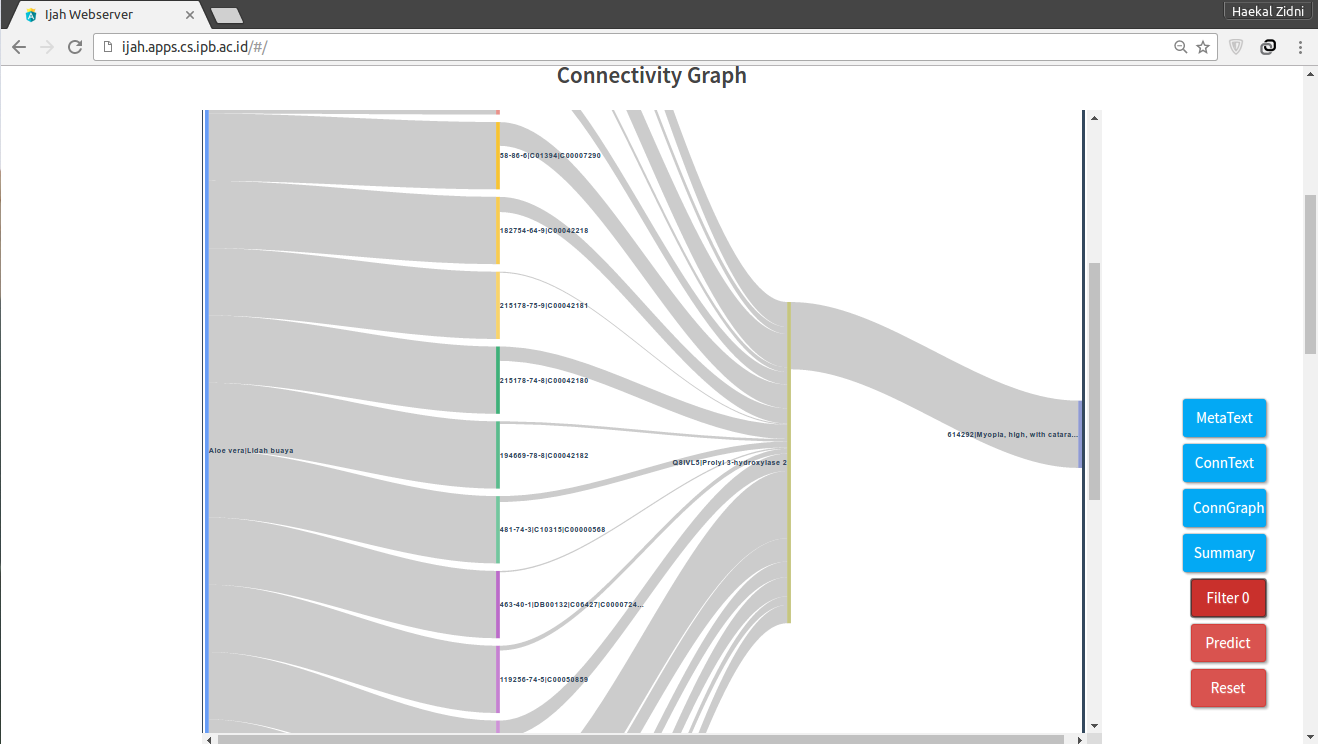
\includegraphics[scale=0.3]{ijah_filter_0.png}
	\caption{Filter 0, menampilkan semua konektivitas}
	\label{fig:ijah_filter_0}
	\end{figure}

	\begin{figure}[H]
	\centering
	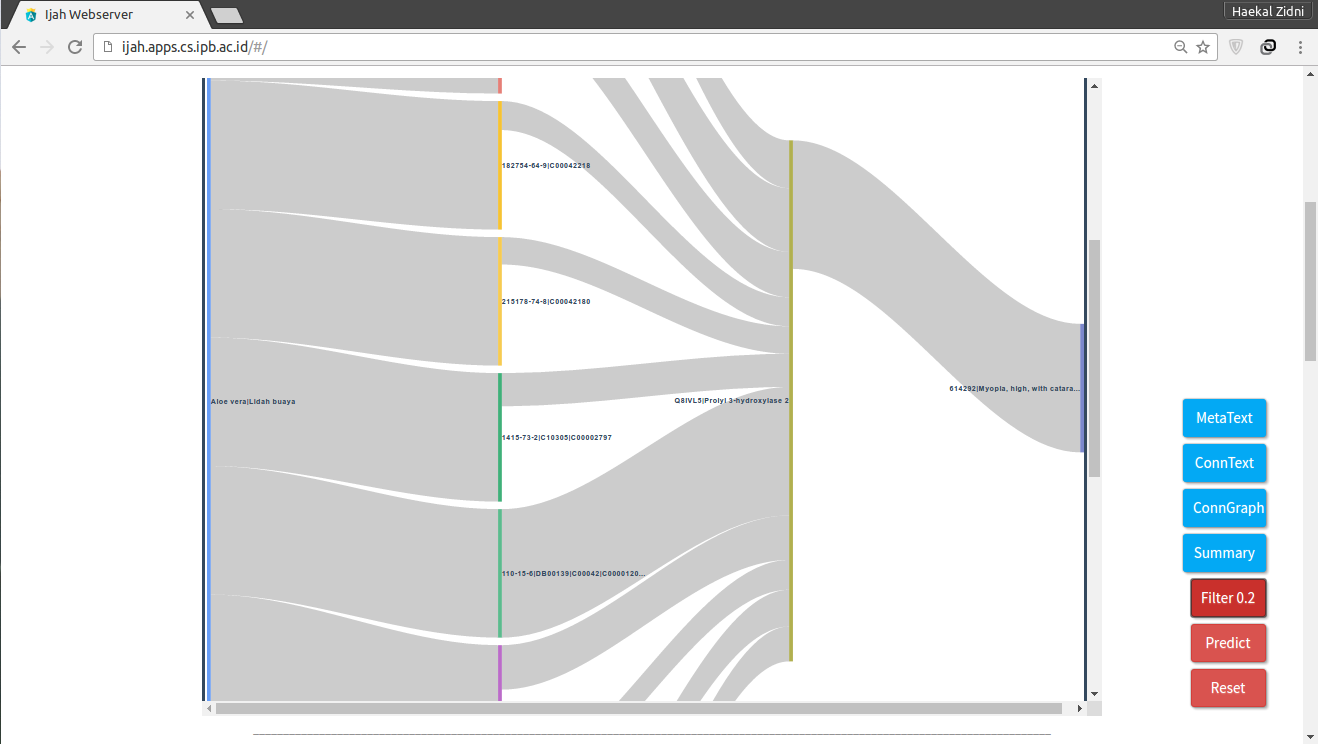
\includegraphics[scale=0.3]{ijah_filter_02.png}
	\caption{Filter 0.2, menampilkan konektivitas minimal 0.2, output mulai berkurang}
	\label{fig:ijah_filter_02}
	\end{figure}

	\begin{figure}[H]
	\centering
	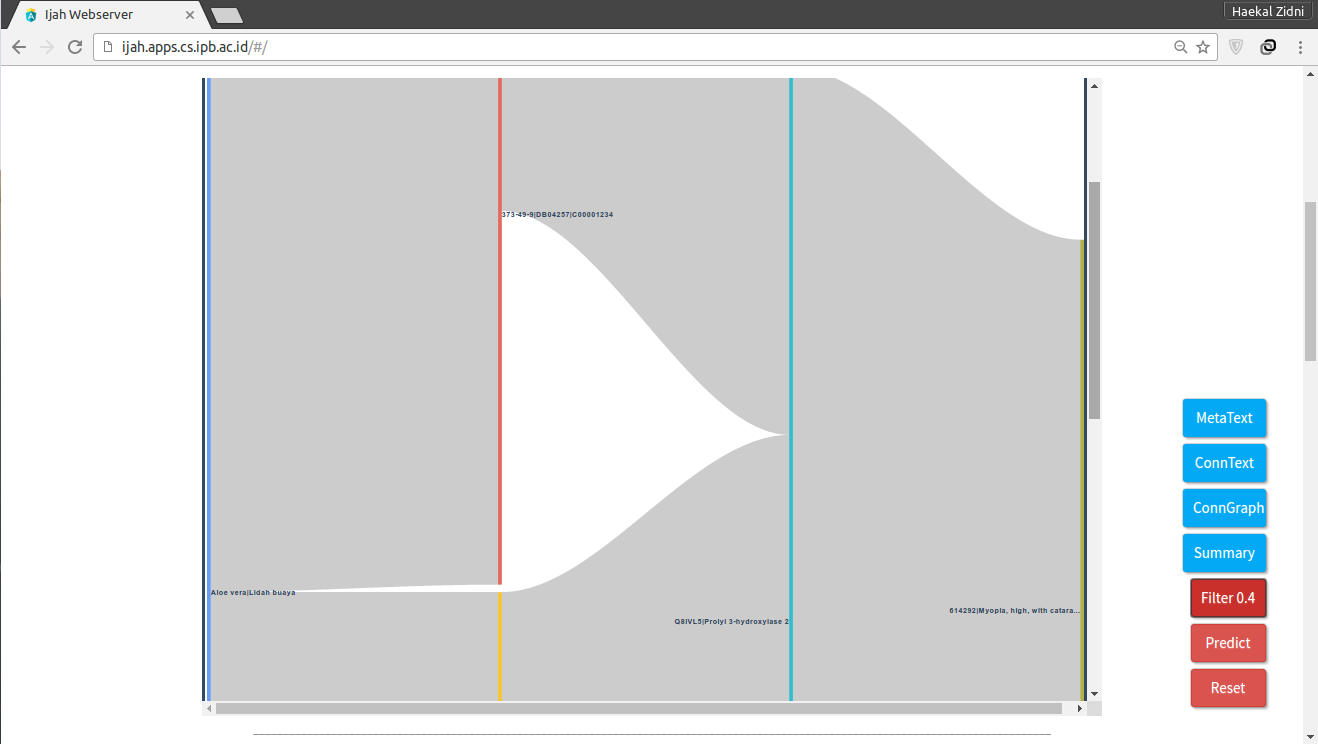
\includegraphics[scale=0.3]{ijah_filter_04.png}
	\caption{Filter 0.4, menampilkan konektivitas minimal 0.4, output jauh berkurang karena konektivitas dengan skor minimal 0.4 semakin sedikit}
	\label{fig:ijah_filter_04}
	\end{figure}

	\begin{figure}[H]
	\centering
	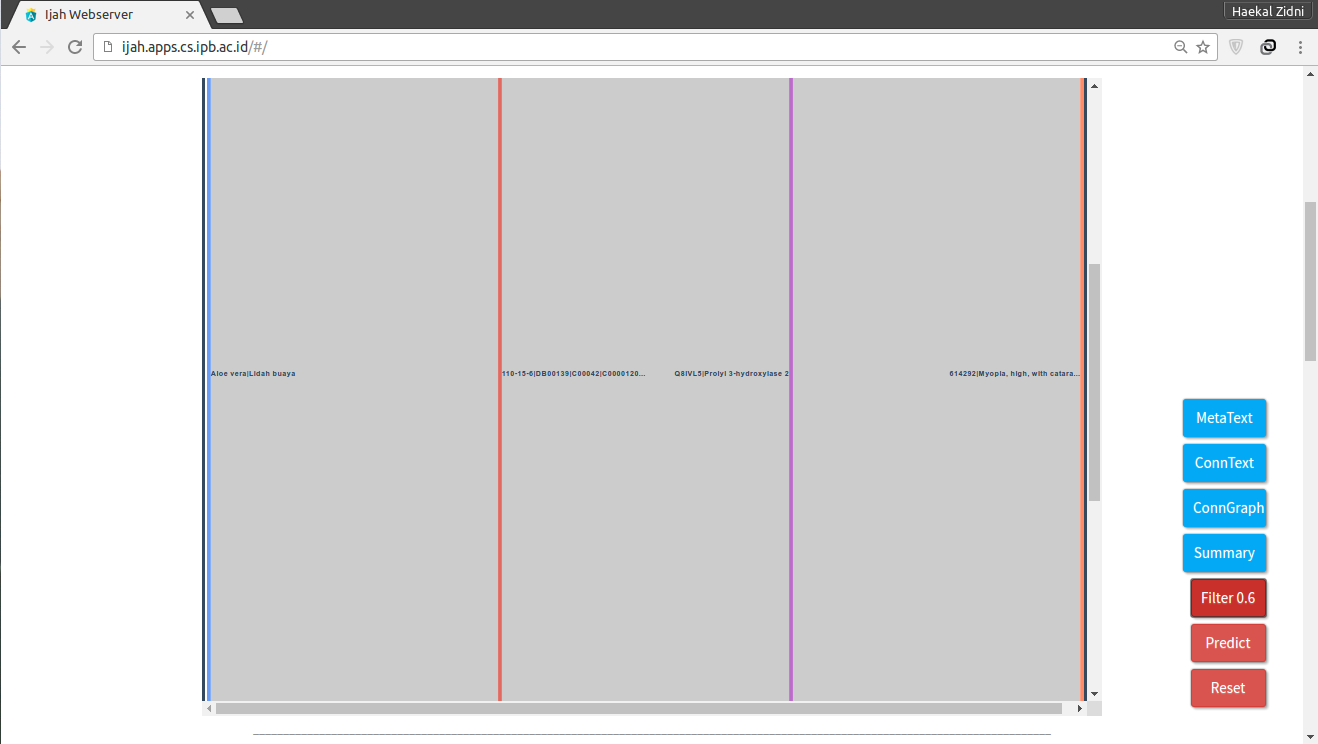
\includegraphics[scale=0.3]{ijah_filter_06.png}
	\caption{Filter 0.6, menampilkan konektivitas minimal 0.6, hanya ada satu output yang muncul. Dalam kasus ini output yang tersisa hanya yang bernilai 1 (100\% terkoneksi) sehingga filter 0.8 dan filter 1 memunculkan hasil yang sama}
	\label{fig:ijah_filter_02}
	\end{figure}

	\subsection{Predict} \label{predictmore}
	Ketika tombol eksekusi dijalankan, ada batas waktu prediksi 5 detik. Terkadang belum semua prediksi termuat pada saat output muncul, sehingga tombol \textbf{Predict} memberikan kesempatan untuk melanjutkan prediksi kembali selama 5 detik. Output yang dihasilkan mungkin akan bertambah seiring bertambahnya hasil prediksi.

	\begin{figure}[H]
	\centering
	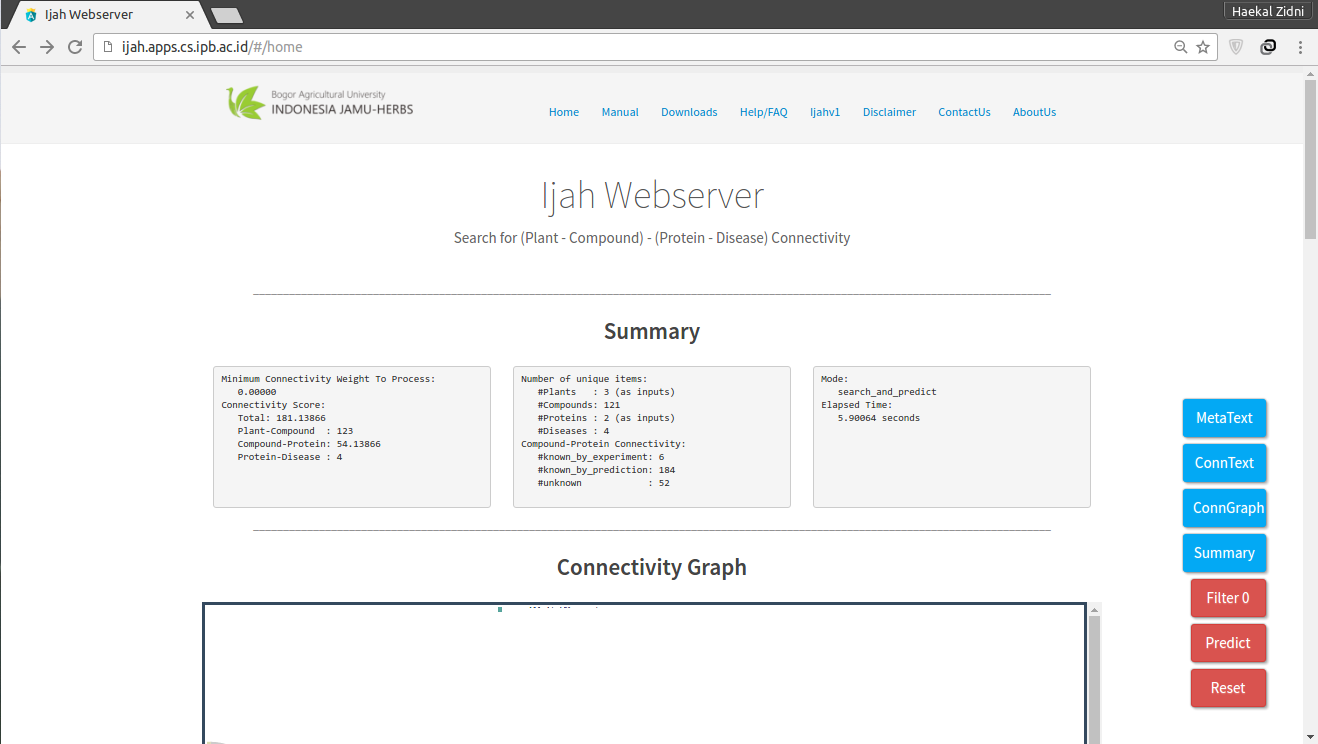
\includegraphics[scale=0.3]{ijah_predict_01.png}
	\caption{Salah satu contoh output. Nilai awal yaitu Known By Prediction sebanyak 184, dengan nilai konektivitas yang belum diketahui (Unknown) sebesar 52}
	\label{fig:ijah_predict_01}
	\end{figure}

	\begin{figure}[H]
	\centering
	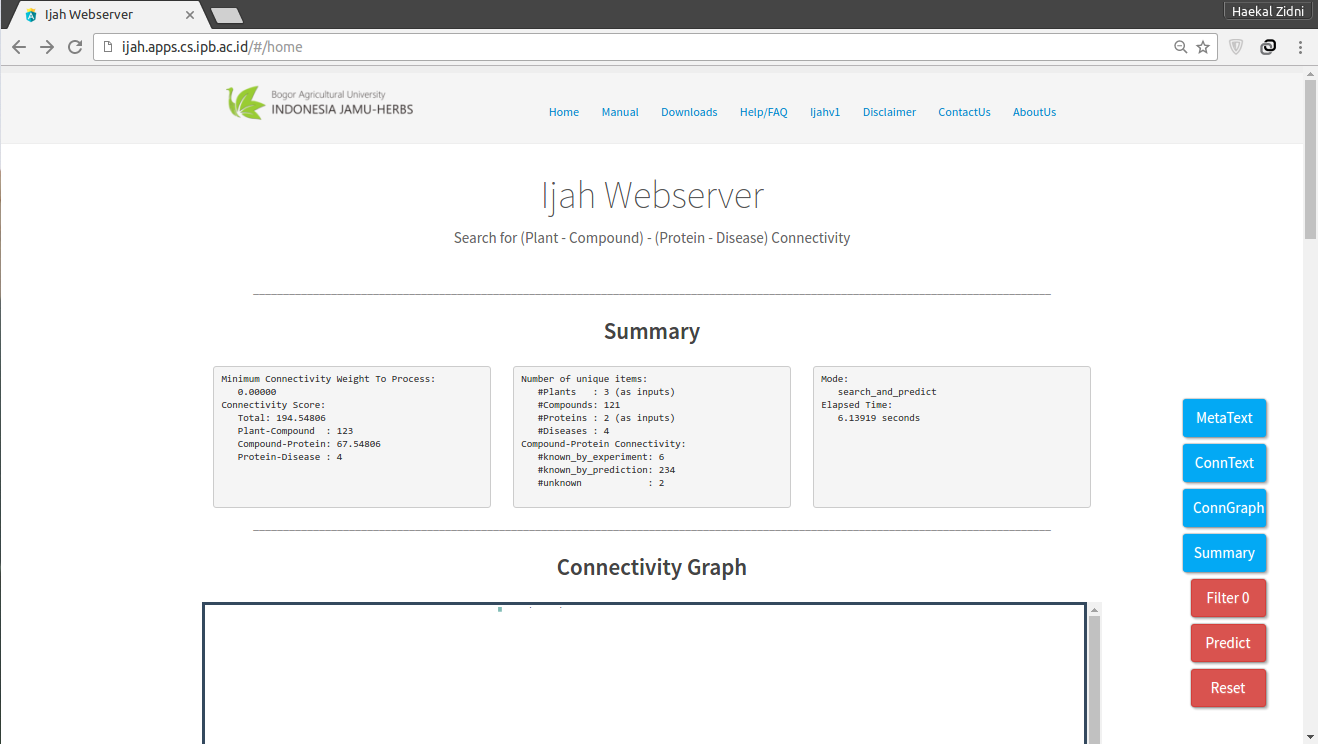
\includegraphics[scale=0.3]{ijah_predict_02.png}
	\caption{Setelah dijalankan tombol Predict dan melakukan 5 detik prediksi tambahan, nilai Known By Prediction meningkat menjadi 234 dan Unknown berkurang hingga tersisa 2 saja}
	\label{fig:ijah_predict_02}
	\end{figure}

%% This is an example first chapter.  You should put chapter/appendix that you
%% write into a separate file, and add a line \include{yourfilename} to
%% main.tex, where `yourfilename.tex' is the name of the chapter/appendix file.
%% You can process specific files by typing their names in at the 
%% \files=
%% prompt when you run the file main.tex through LaTeX.
\chapter{Menu-menu}  \label{chap:Menu}

\section{Manual}
Menu \emph{Manual} berisi \emph{link} untuk mendownload file Manual penggunaan Ijah Webserver. Kedepannya, isi file Manual juga akan ditampilkan di halaman ini.

\begin{figure}[H]
	\centering
	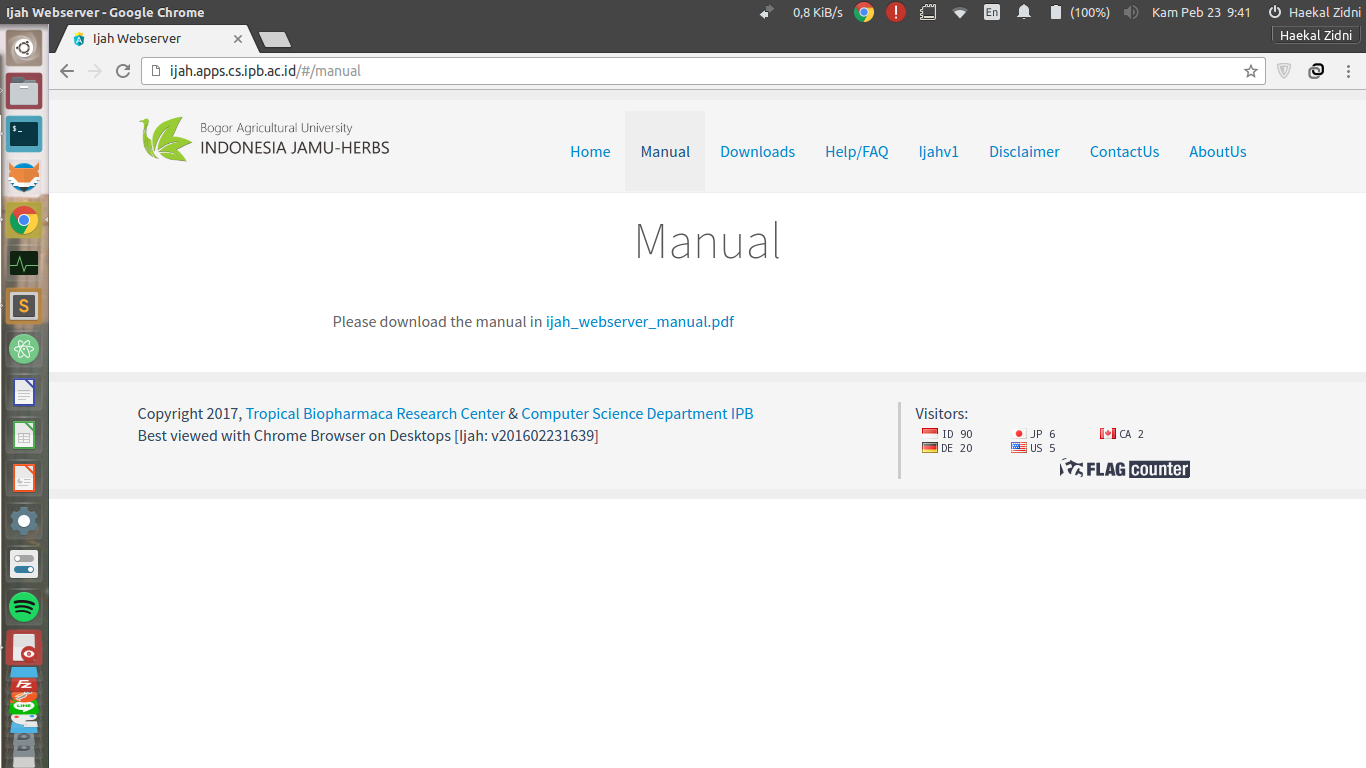
\includegraphics[scale=0.3]{ijah_manual_page.png}
	\caption{Halaman Manual}
	\label{fig:ijah_manual_page}
\end{figure}

\section{Downloads} \label{Downloads}
Menu \emph{Downloads} menyediakan link untuk mengunduh Metadata seluruh item (tanaman, senyawa, protein, dan penyakit) yang ada dalam database Ijah Webserver. Juga disediakan data seluruh konektivitas (keterhubungan) antar item dan data lainnya seperti similarity data, data sekuens protein, dan lain lain.

Untuk mengunduh file pada halaman ini cukup klik nama file yang ingin diunduh

\begin{figure}[H]
	\centering
	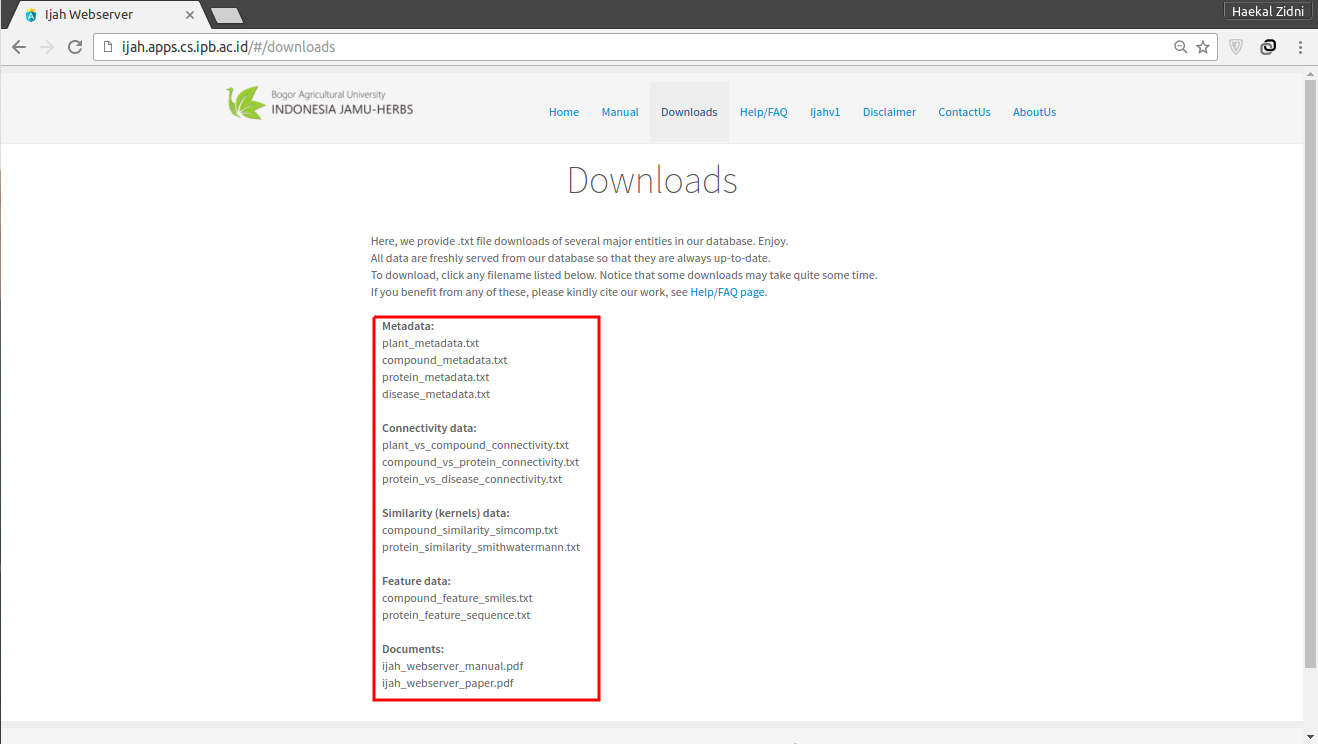
\includegraphics[scale=0.3]{ijah_downloadpage.png}
	\caption{Daftar file yang dapat di\-download}
	\label{fig:ijah_downloadpage}
\end{figure}

	\subsection{Metadata}
	File yang dapat didownload pada kategori Metadata yaitu:

	\begin{itemize}
	\item \textbf{plant\_metadata.txt} -- Berisi metadata seluruh tanaman pada \emph{database} Ijah Webserver. 
	\item \textbf{compound\_metadata.txt} -- Berisi metadata seluruh senyawa (\emph{compound}) pada \emph{database} Ijah Webserver.
	\item \textbf{protein\_metadata.txt} -- Berisi metadata seluruh bioprotein pada \emph{database} Ijah Webserver.
	\item \textbf{disease\_metadata.txt} -- Berisi metadata seluruh penyakit pada \emph{database} Ijah Webserver.
	\end{itemize}

	\subsection{Connectivity Data}
	File yang dapat didownload pada kategori Connectivity Data yaitu:

	\begin{itemize}
	\item \textbf{plant\_vs\_compound\_connectivity.txt} -- Berisi data konektivitas tanaman dengan senyawa beserta skor konektivitasnya pada \emph{database} Ijah Webserver.
	\item \textbf{compound\_vs\_protein\_connectivity.txt} -- Berisi data konektivitas senyawa dengan protein beserta skor konektivitasnya pada \emph{database} Ijah Webserver.
	\item \textbf{protein\_vs\_disease\_connectivity.txt} -- Berisi data konektivitas protein dengan penyakit beserta skor konektivitasnya pada \emph{database} Ijah Webserver.
	\end{itemize}

	\subsection{Similarity (kernels) data}
	\begin{itemize}
	\item compound\_similarity\_simcomp.txt  
	\item protein\_similarity\_smithwatermann.txt  
	\end{itemize}

	\subsection{Feature data}
	\begin{itemize}
	\item compound\_feature\_smiles.txt  
	\item protein\_feature\_sequence.txt  
	\end{itemize}

	\subsection{Documents}
	Dokumentasi Ijah Webserver
	\begin{itemize}
	\item \textbf{ijah\_webserver\_manual.pdf} -- Manual penggunaan Ijah Webserver
	\item \textbf{ijah\_webserver\_paper.pdf} -- Paper penelitian Ijah Webserver
	\end{itemize}

\section{Help/FAQ}
Menu \emph{Help/FAQ} berisikan beberapa pertanyaan umum \emph{(Frequently Asked Questions)} beserta jawabannya.

\begin{figure}[H]
	\centering
	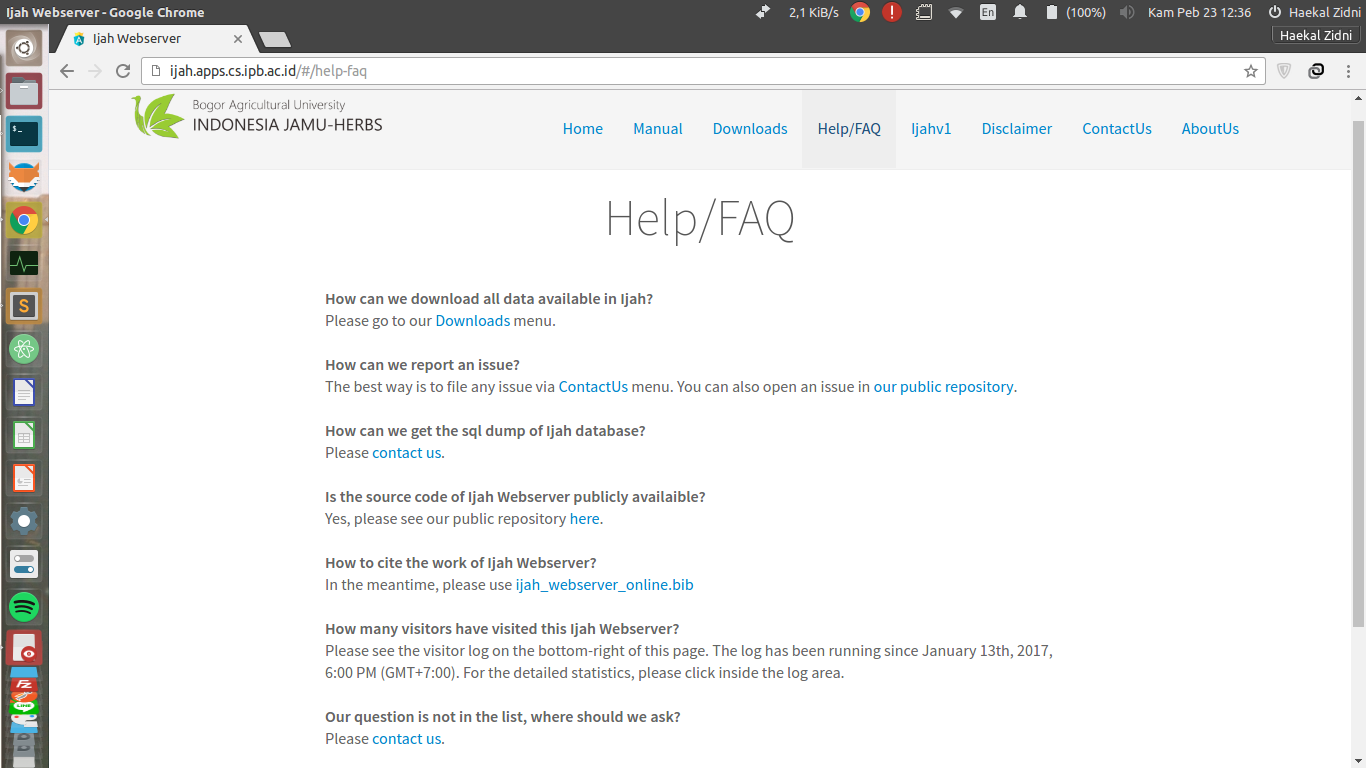
\includegraphics[scale=0.3]{ijah_faq.png}
	\caption{Halaman Help/FAQ}
	\label{fig:ijah_faq}
\end{figure}

Menu FAQ ini tersedia dalam bahasa Inggris, berikut terjemahan dari pertanyaan pada menu FAQ menurut Ijah Webserver versi ini:

\begin{itemize}
\item {\textbf{Q:}} Bagaimana cara mengunduh semua data yang ada pada Ijah?\\
A: Silakan menuju menu \textbf{\nameref{Downloads}}.
\item {\textbf{Q:}} Bagaimana cara melaporkan isu dan masalah?\\
A: Cara termudah yaitu dengan mengontak kami di menu \textbf{\nameref{ContactUs}}. Anda bisa juga menyampaikannya di repositori \emph{code} kami. (Menuju repositori -- lihat bab \ref{sec:ws_source}).
\item {\textbf{Q:}} Bagaimana cara mendapatkan \emph{SQL dump} dari \emph{database} Ijah?\\
A: Silakan kontak tim kami di menu \textbf{\nameref{ContactUs}}.
\item {\textbf{Q:}} Apakah \emph{source code} Ijah tersedia secara publik?\\
A: Ya, silakan lihat repositori publik kami disini (Menuju repositori -- silakan lihat bab \ref{sec:ws_source}).
\item {\textbf{Q:}} Bagaimana cara mengutip karya Ijah Webserver?\\
A: Untuk saat ini silakan lihat di \href{http://ijah.apps.cs.ipb.ac.id/api/ijah_webserver_online.bib}{\textbf{ijah\_webserver\_online.bib}}
\item {\textbf{Q:}} Berapa kali Ijah Webserver telah dikunjungi?\\
A: Silakan lihat \emph{visitor log} pada bagian kanan-bawah halaman Ijah Webserver. \emph{Log} ini telah berjalan sejak 13 Januari 2017 pukul 18:00 (zona waktu GMT+7:00). Untuk statistik detail silakan klik pada area \emph{visitor log}. (\emph{Visitor log} ada pada bab \ref{ssec:visitor log})
\item {\textbf{Q:}} Mengapa tata halaman terlihat berantakan? Bagaimana solusinya?\\
A: Kami sedang berusaha mengerjakan tata halaman yang adaptif dan bisa menyesuaikan dengan resolusi monitor. Untuk sementara waktu, mohon gunakan \emph{zoom out/in} pada \emph{browser} anda.
\item {\textbf{Q:}} Pertanyaan saya tidak ada pada halaman ini, dimana kami bisa mengajukan pertanyaan?\\
A: Silakan kontak kami di menu \textbf{\nameref{ContactUs}}.
\end{itemize}

\section{Ijahv1}
Menu \emph{Ijahv1} berisi link menuju versi awal Ijah (Ijah versi 1, atau Ijahv1)

\begin{figure}[H]
	\centering
	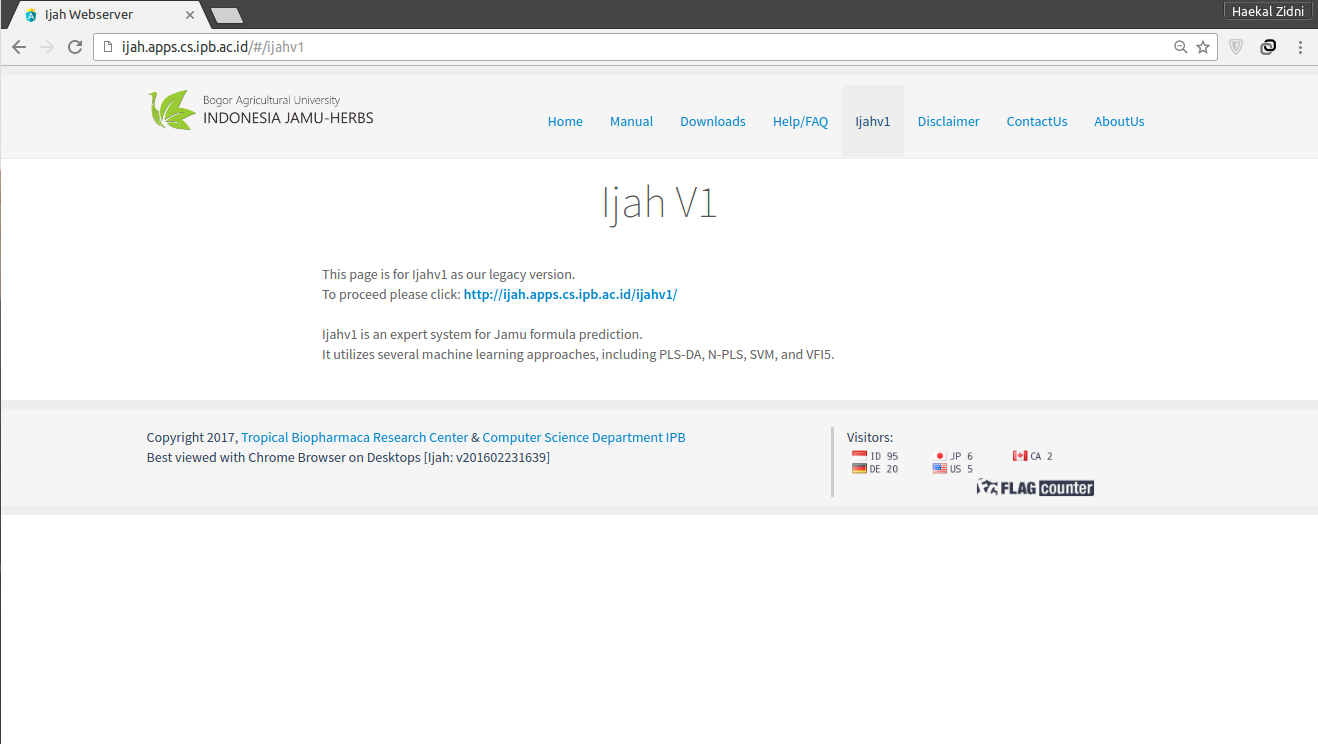
\includegraphics[scale=0.3]{ijah_v1.png}
	\caption{Isi halaman menu Ijahv1}
	\label{fig:ijah_v1}
\end{figure}

Jika anda ingin mengakses Ijahv1 silakan mengunjungi \href{http://ijah.apps.cs.ipb.ac.id/ijahv1/}{\textbf{http://ijah.apps.cs.ipb.ac.id/ijahv1/}}

\section{Disclaimer}

Menu \emph{Disclaimer} berisikan pernyataan batasan \emph{responsibility} pihak Ijah Webserver atas penggunaan hasil \emph{output} dari Ijah Webserver.

\begin{figure}[H]
	\centering
	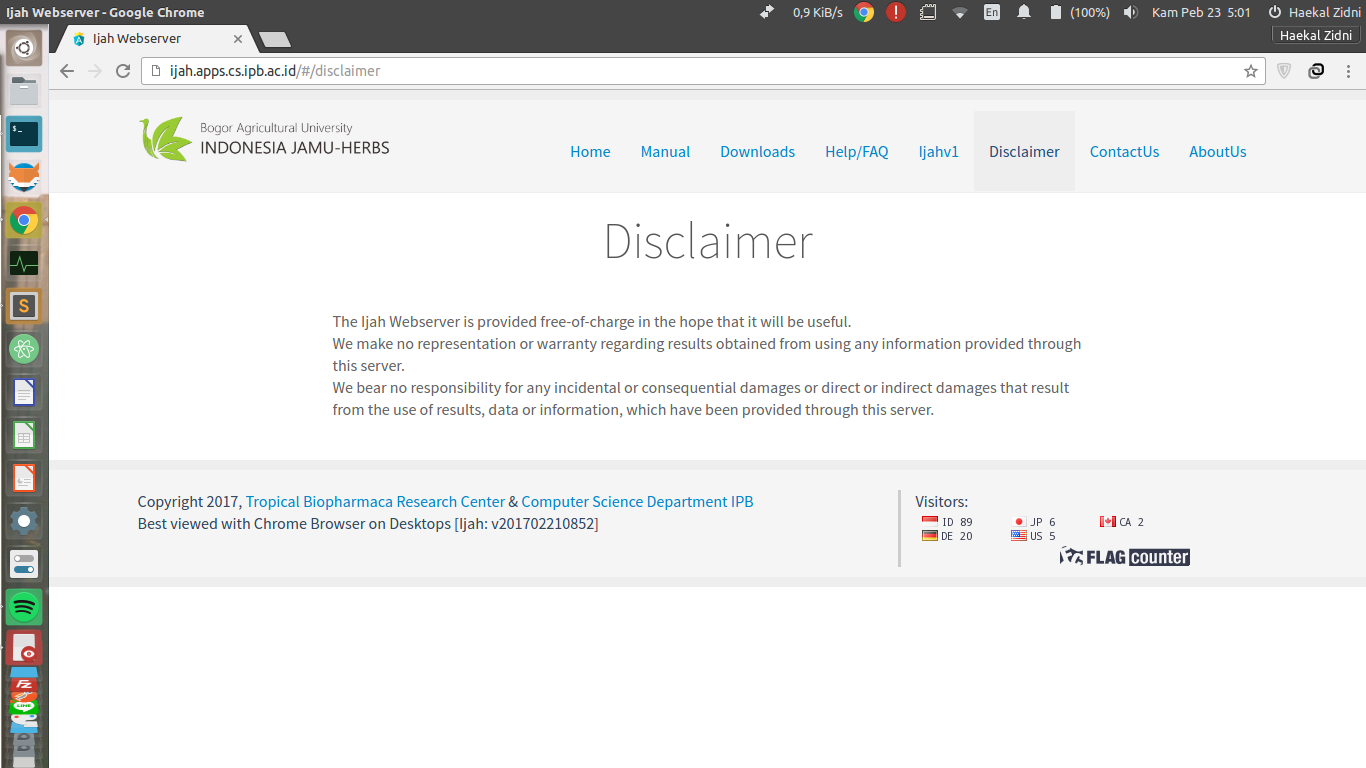
\includegraphics[scale=0.3]{ijah_disclaimer.png}
	\caption{Isi halaman Disclaimer}
	\label{fig:ijah_disclaimer}
\end{figure}

Terjemahan dari isi halaman Disclaimer yaitu:

\textit{``Ijah Webserver ini gratis, dengan harapan dapat membantu banyak pihak. Namun kami tidak menjamin akibat dari penggunaan informasi dari Webserver ini. Dan kami tidak bertanggungjawab atas insiden atau kerusakan baik langsung maupun tidak langsung yang diakibatkan oleh penggunaan data atau informasi yang kami sediakan di Webserver ini.''}


\section{ContactUs} \label{ContactUs}

Menu \emph{ContactUs} merupakan sarana komunikasi antara pengguna dengan tim pengembang Ijah Webserver. Dengan mengisikan tanggapan/keluhan/saran pada form Contact Us, tanggapan anda akan terkirim ke E-mail kami.

\begin{figure}[H]
	\centering
	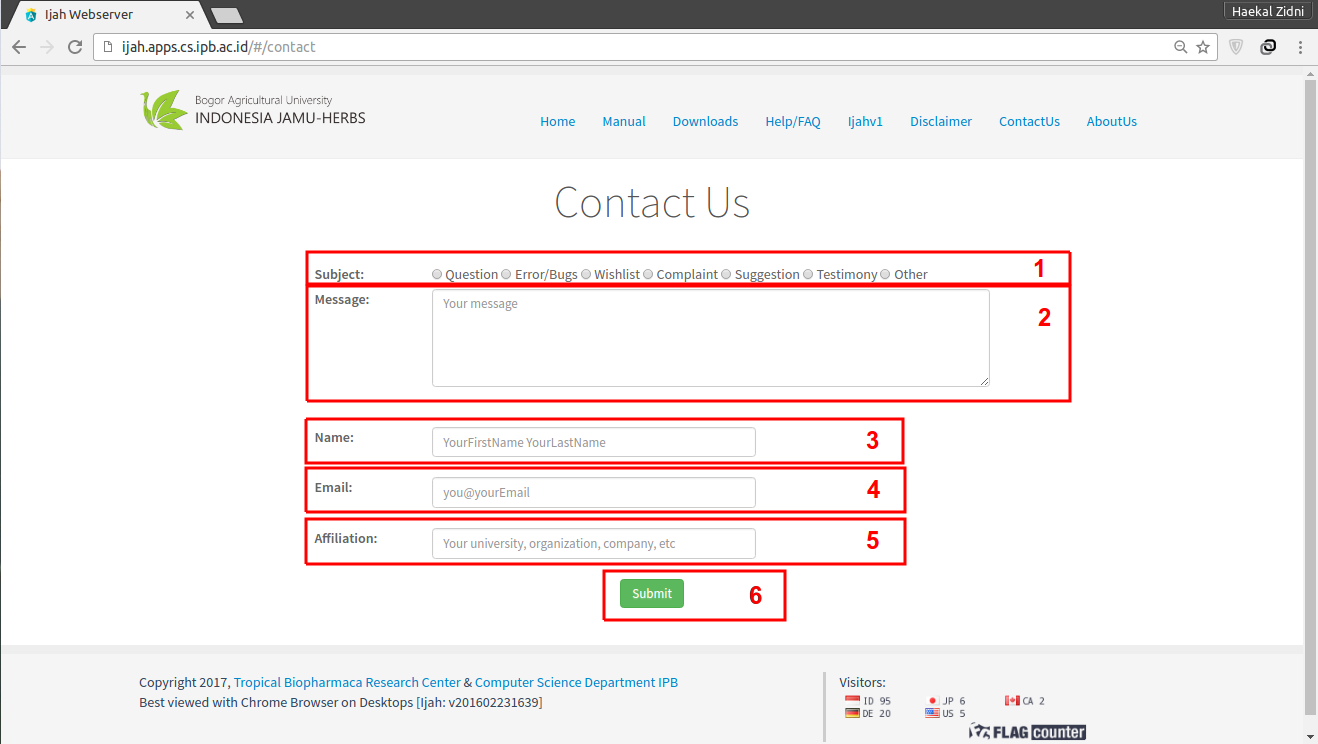
\includegraphics[scale=0.3]{ijah_contact_page.png}
	\caption{Halaman ContactUs pada Ijah Webserver:
	(1) \hyperref[subject]{Pemilihan Subject};
	(2) \hyperref[message]{Message box};
	(3) \hyperref[personal data]{Name box};
	(4) \hyperref[personal data]{E-mail box};
	(5) \hyperref[personal data]{Affiliation box};
	(6) \hyperref[submit]{Tombol Submit};
	}
	\label{fig:ijah_contact_page}
\end{figure}

	\subsection{Topik} \label{subject}
	Pada bagian \emph{Subject} anda akan memilih topik tanggapan anda 
	\begin{itemize}
	\item \textbf{Question:} mengajukan pertanyaan.
	\item \textbf{Error/Bugs:} memberitahukan adanya kesalahan.
	\item \textbf{Wishlist:} menyampaikan saran fitur apa yang diinginkan pada versi selanjutnya.
	\item \textbf{Complaint:} menyampaikan keluhan dalam penggunaan.
	\item \textbf{Suggestion:} memberikan saran.
	\item \textbf{Testimony:} memberikan testimoni tentang Ijah Webserver.
	\item \textbf{Other:} untuk menyampaikan hal lain yang tidak termasuk dalam kategori diatas.
	\end{itemize}

	\subsection{Isi Pesan} \label{message}
	Isikan pesan anda pada bagian \emph{Message}. Jumlah karakter tidak dibatasi, jadi mohon untuk tidak menggunakan singkatan jika tidak diperlukan demi memudahkan tim kami dalam membaca tanggapan anda. 


	\subsection{Isi Data Diri Anda} \label{personal data}
	Setelah menuliskan tanggapan, silakan isi data diri anda, nama pada bagian \emph{Name}, alamat E\-mail anda pada bagian \emph{E\-mail}, dan afiliasi anda (organisasi, universitas, atau perusahaan) pada bagian \emph{Affiliation}.

	\textbf{Penting:} Nama dan alamat E-mail \emph{wajib} diisi. 

	\subsection{Kirim Tanggapan} \label{submit}
	Setelah semua data terisi lengkap, tekan \textbf{Submit} dan tanggapan anda akan terkirim.

\section{AboutUs}

Menu \emph{AboutUs} berisi info tentang tim pengembang Ijah Webserver

\begin{figure}[H]
	\centering
	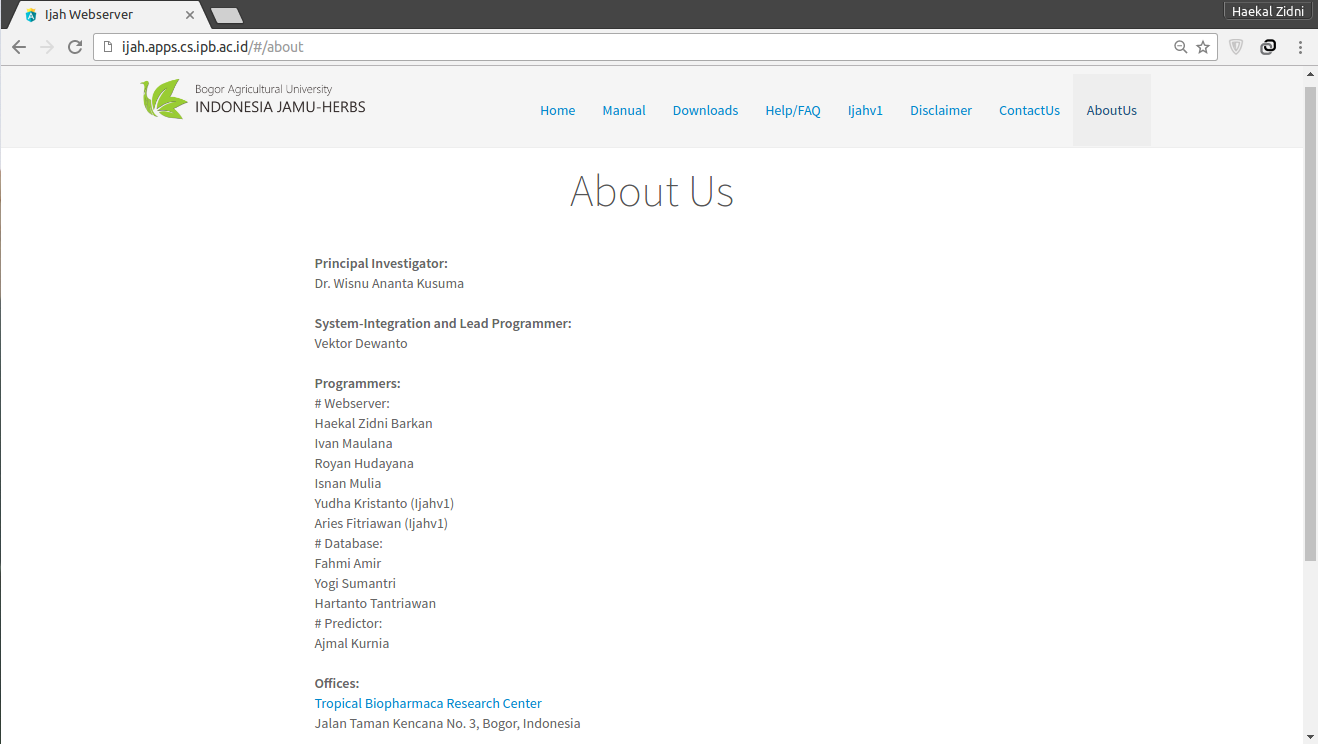
\includegraphics[scale=0.3]{ijah_about.png}
	\caption{Isi halaman About Us}
	\label{fig:ijah_about}
\end{figure}

Tim pengembang Ijah Webserver yaitu:

\begin{itemize}
\item Principal Investigator:\\ 
Dr. Wisnu Ananta Kusuma

\item System-Integration and Lead Programmer:\\
Vektor Dewanto

\item Programmers:\\
\# Webserver:
\begin{itemize}
\item Haekal Zidni Barkan
\item Ivan Maulana
\item Royan Hudayana
\item Isnan Mulia
\item Yudha Kristanto (Ijahv1)
\item Aries Fitriawan (Ijahv1)
\end{itemize}
\# Database:
\begin{itemize}
\item Fahmi Amir
\item Yogi Sumantri
\item Hartanto Tantriawan
\end{itemize}
\# Predictor:
\begin{itemize}
\item Ajmal Kurnia
\end{itemize}
\end{itemize}

% \emph{Use case} ini melibatkan hanya satu sisi yaitu \emph{Drug-side} saja. pada \emph{use case} ini, input dari salah satu \emph{drug-side} (Plant atau Compound) harus ada.

% \section{Plant Search Only}

% Pada contoh ini, input dari \emph{drug-side} berupa tanaman (Plant). Contoh ini mencari dari tanaman yang diinputkan, apa saja senyawa yang terkandung dalam tanaman itu, dan senyawa tersebut dapat berkhasiat untuk penyakit apa melalui protein apa.

% \subsection{Input}
% \begin{figure}[H]
% 	\centering
% 	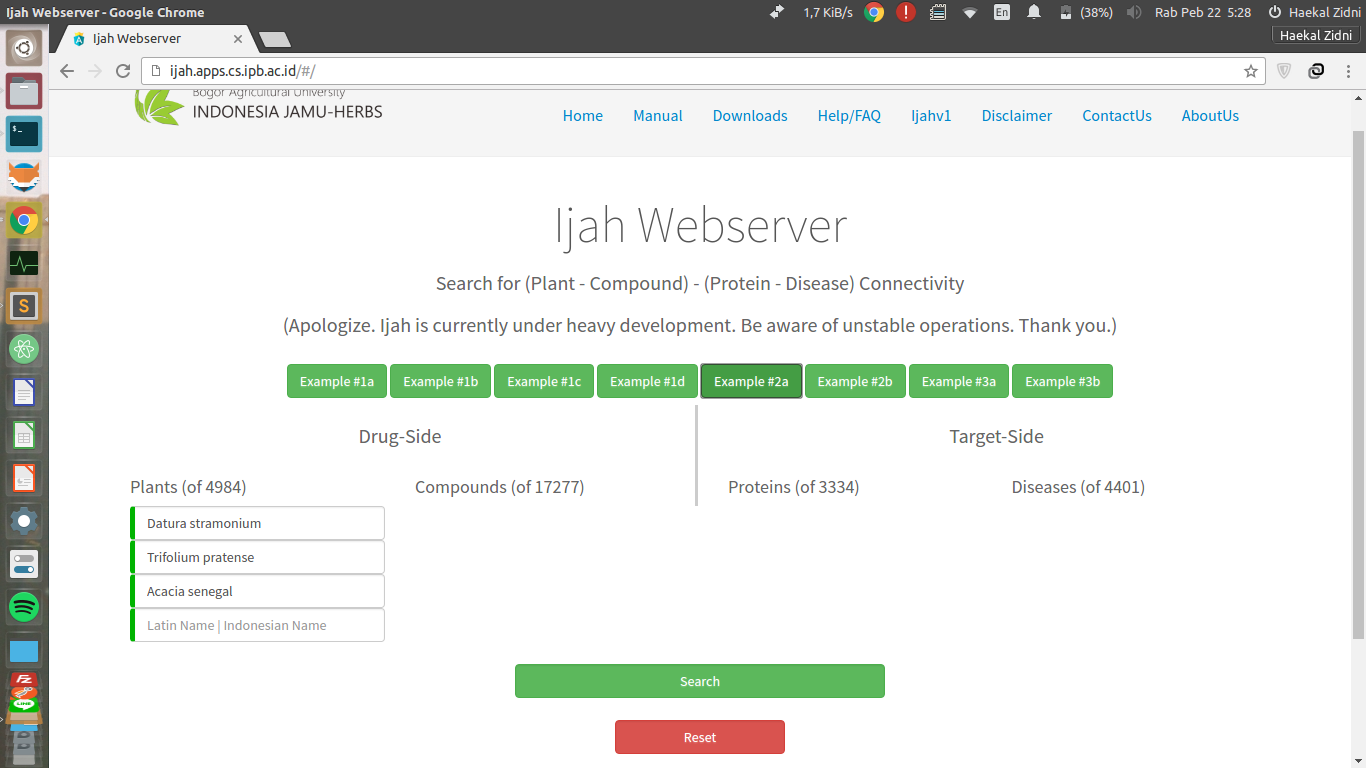
\includegraphics[scale=0.3]{example_2a.png}
% 	\caption{Contoh \emph{use case} input Plant Search Only}
% 	\label{fig:example_2a}
% \end{figure}

% Seperti yang telah dibahas pada bab sebelumnya, untuk jenis \emph{use case} ini tombol hanya bertuliskan \textbf{Search}, bukan Search and Predict seperti \emph{use case} sebelumnya.

% \subsection{Output}
% Output pada contoh \emph{search} dari 3 jenis tanaman ini adalah sebagai berikut, dimulai dari \emph{Connectivity Graph Output}

% \begin{figure}[H]
% 	\centering
% 	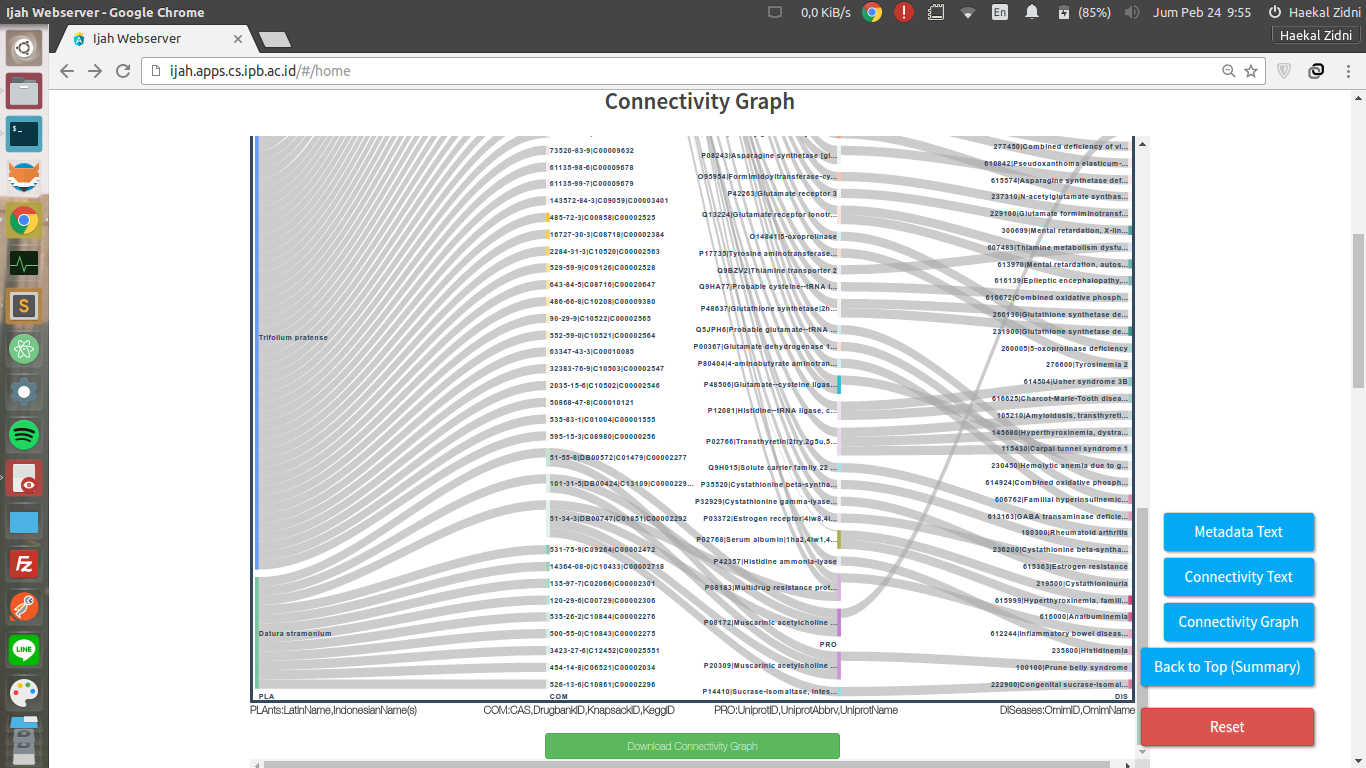
\includegraphics[scale=0.3]{ijah_example_2a_graph.png}
% 	\caption{Connectivity Graph Output pada use case Plant Search Only}
% 	\label{fig:ijah_example_2a_output}
% \end{figure}

% Graf yang dihasilkan kali ini cukup besar karena menampilkan semua penyakit yang terkait dengan seluruh senyawa yang dikandung tanaman-tanaman tersebut. Karena contoh ini menampilkan semua yang terkait dengan tanaman yang diinputkan.

% Hasil \emph{Connectivity Text Output} untuk contoh ini:

% \begin{figure}[H]
% 	\centering
% 	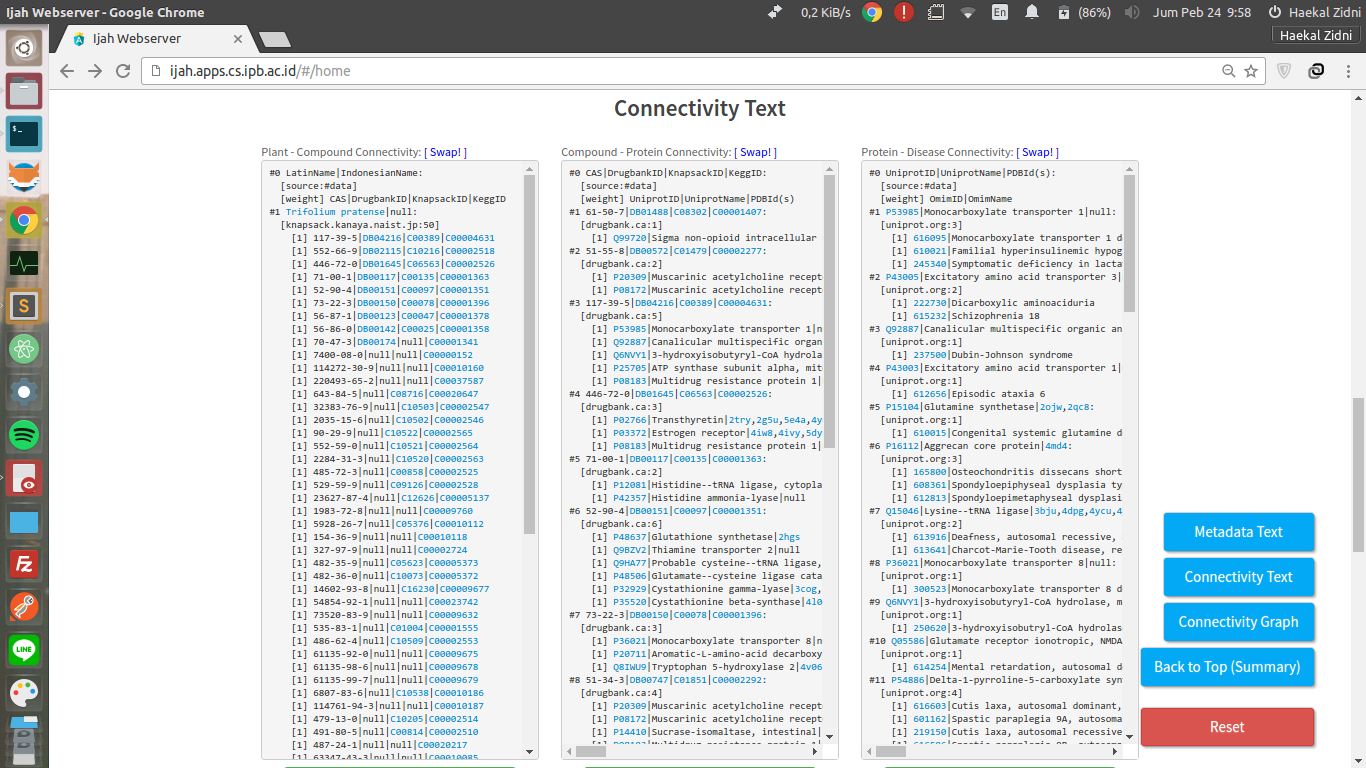
\includegraphics[scale=0.3]{ijah_example_2a_text.png}
% 	\caption{Connectivity Text Output pada use case Plant Search Only}
% 	\label{fig:ijah_example_2a_text}
% \end{figure}

% Hasil \emph{Metadata Text Output} untuk contoh ini:

% \begin{figure}[H]
% 	\centering
% 	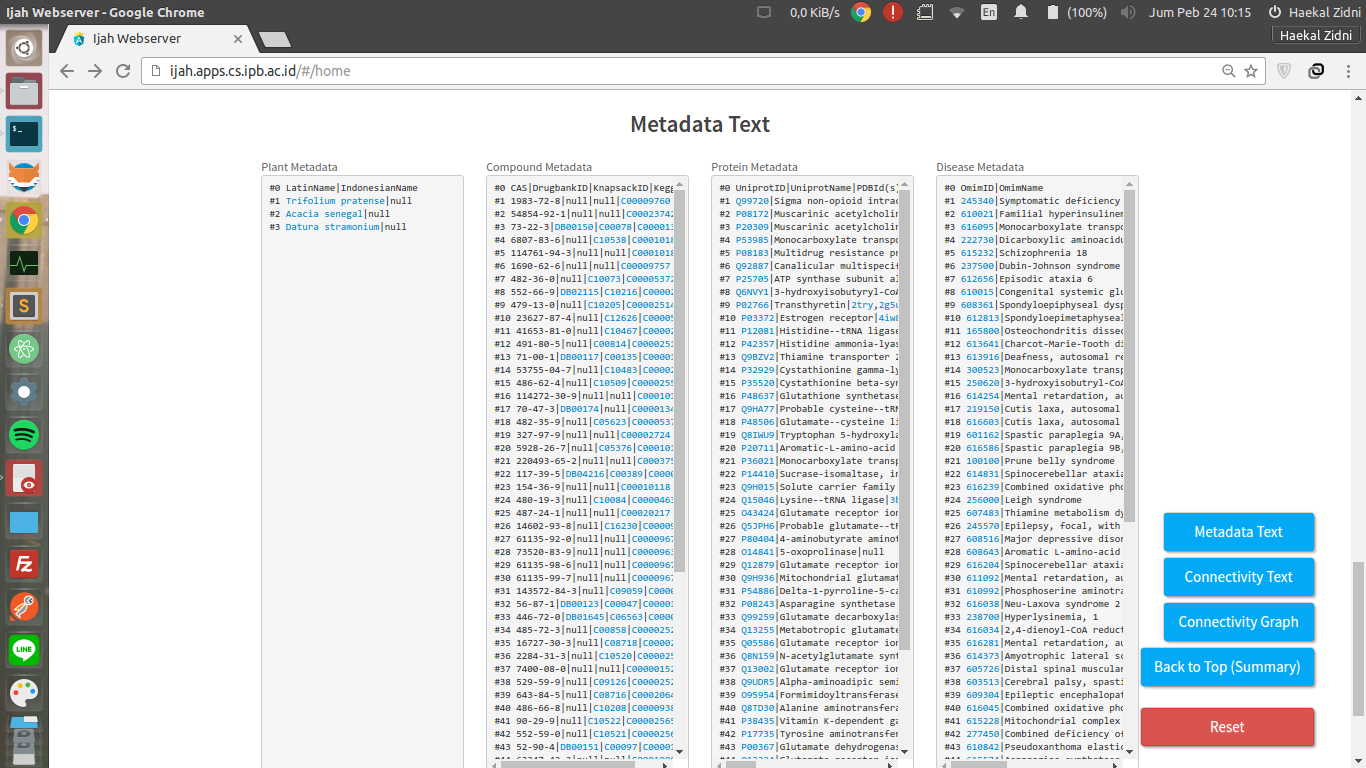
\includegraphics[scale=0.3]{ijah_example_2a_meta.png}
% 	\caption{Metadata Text Output pada use case Plant Search Only}
% 	\label{fig:ijah_example_2a_meta}
% \end{figure}

% \section{Compound Search Only}
% Contoh lain dari \emph{use case} Drug-Side Only yaitu Compound Search Only dimana perbedaannya hanya pada input, yaitu menginputkan senyawa (Compound) untuk mencari semua (Plant, Protein, Disease) yang terkait dengan senyawa yang diinputkan.


%% This is an example first chapter.  You should put chapter/appendix that you
%% write into a separate file, and add a line \include{yourfilename} to
%% main.tex, where `yourfilename.tex' is the name of the chapter/appendix file.
%% You can process specific files by typing their names in at the 
%% \files=
%% prompt when you run the file main.tex through LaTeX.
\chapter{Pangkalan Data \emph{(Database)} Rujukan} \label{db chapter}

Repositori untuk \emph{database} Ijah Webserver dapat dilihat di \textbf{\url{https://github.com/tttor/csipb-jamu-prj/tree/master/database}}. Repositori \emph{database} Ijah terbagi menjadi tiga bagian yaitu:

\begin{itemize}
\item {\textbf{Crawler}} -- berisi \emph{code} untuk menarik data \emph{(crawling)} dari pangkalan data yang menjadi referensi.
\item {\textbf{Inserter}} -- berisi \emph{code} untuk memasukkan data hasil \emph{crawling} ke dalam \emph{database} Ijah.
\item {\textbf{Ref}} -- berisi referensi pangkalan data yang digunakan. Referensi ini akan terus diperbarui.
\end{itemize}

\section{Data Konektivitas}
Konektivitas (\emph{connectivity}) antar entitas, sering juga disebut interaksi (\emph{interaction}) atau relasi (\emph{relation}), menyatakan hubungan atau keterkaitan antar dua entitas, dalam konteks ini hubungan dari entitas pada Drug-side dengan entitas pada Target-side.

Hingga versi ini, pangkalan data yang sudah dimasukkan sebagai rujukan yaitu KNApSAcK, DrugBank, KEGG, Uniprot, OMIM, CAS, dan  PDB.

% Hingga versi ini, pangkalan data yang sudah dimasukkan sebagai rujukan yaitu \hyperref[knapsack]{KNApSAcK}, \hyperref[drugbank]{DrugBank}, \hyperref[kegg]{KEGG}, \hyperref[uniprot]{Uniprot}, \hyperref[omim]{OMIM}, \hyperref[cas]{CAS}, dan \hypperref[pdb]{PDB}.
	\subsection{\emph{Plant-Compound connectivity}}
		\subsubsection{Knapsack} \label{knapsack}
		KNApSAcK adalah pangkalan data yang berisi informasi hubungan antara spesies tanaman dengan metabolit, yang sangat berguna untuk membantu riset metabolomik. Inti pangkalan data KNApSAcK saat ini telah berisi 101,500 data hubungan spesies-metabolit yang mencakup 20,741 spesies tanaman dan 50,048 metabolit. KNApSAcK dapat diakses di alamat URL \textbf{\url{http://kanaya.naist.jp/KNApSAcK_Family/}}.

		\subsubsection{StreptomeDB} \label{streptome_db}
		StreptomeDB adalah pangkalan data bioinformatika farmasi yang memiliki fitur sebagai berikut:
		\begin{itemize}
		\item 1,600 produk alami
		\item 600 organisme produsen
		\item 1,000 referensi literatur
		\item 350 aktivitas
		\item 1,800 konektivitas senyawa-aktivitas
		\item 400 konektivitas senyawa-rute sintetis 
		\item sistem klasifikasi filogenetik untuk ratusan spesies
		\end{itemize}
		StreptomeDB dapat diakses di alamat URL \textbf{\url{http://www.pharmaceutical-bioinformatics.de/streptomedb/}}.

		\subsubsection{Dr. Duke's Phytochemical and Ethnobotanical Databases} \label{pedb}
		Pangkalan data ini berisi informasi tanaman etnobotani, penggunaan secara etnobotanikal, senyawa kimia, dan data aktivitas biologi. Disini terdapat 49,788 entri. Dr. Duke's Phytochemical and Ethnobotanical Databases dapat diakses di alamat URL \textbf{\url{https://phytochem.nal.usda.gov/phytochem/search}}.

	\subsection{\emph{Compound-Protein connectivity}}
		\subsubsection{DrugBank} \label{drugbank}
		DrugBank adalah pangkalan data yang berisi informasi obat dan target obat.Sebagai sumber informasi untuk bioinformatika dan \emph{cheminformatics} (informatika kimia), DrugBank menggabungkan rincian data obat (sifat kimia, farmakologi, dan data farmasi) dengan informasi dari target obat (sekuens, struktur, dan \emph{pathway}). DrugBank memiliki cakupan yang luas, referensi yang komprehensif dan deskripsi data yang sangat rinci. DrugBank sendiri banyak digunakan oleh industri obat, ahli kimia obat, apoteker, dokter, mahasiswa, dan masyarakat umum. DrugBank dapat diakses di alamat URL \textbf{\url{http://www.drugbank.ca/}}.

		\subsubsection{Supertarget + Matador} \label{supertarget}
		Supertarget adalah pangkalan data yang berisi informasi hubungan target obat \emph{(drug-target relations)}. Terdiri dari tiga entitas berbeda yaitu \textbf{\emph{Drugs, Proteins,}} dan \textbf{\emph{Side Effects}} (Obat, Protein, dan Efek Samping). Supertarget dapat diakses di alamat URL \textbf{\url{http://insilico.charite.de/supertarget/}}.

		\subsubsection{Transformer} \label{transformer}
		Transformer adalah pangkalan data yang berisi informasi transformasi dan transportasi xenobiotik dalam tubuh manusia. Terdapat pula informasi interaksi enzim fase I dan II dan transporter obat, juga memiliki data obat tradisional Tiongkok. Transformer dapat diakses di alamat URL \textbf{\url{http://bioinformatics.charite.de/transformer/}}.

		\subsubsection{Antibiotic'ome} \label{antibioticome}
		Antibiotic'ome adalah pangkalan data yang menyediakan informasi hubungan retrobiosintesis dari struktur produk alami yang dicocokkan dengan antibiotik yang telah diketahui targetnya, dengan tujuan memprediksi target dari molekul yang diinputkan pengguna. Antibiotic'ome dapat diakses di alamat URL \textbf{\url{https://magarveylab.ca/antibioticome/}}.

		\subsubsection{Therapeutic Target Database (TTD)} \label{ttd}
		Therapeutic Target Database (TTD) adalah pangkalan data yang menyediakan informasi protein therapeutic dan target asam nukleat yang telah dipelajari dan diteliti, penyakit yang ditarget, informasi pathway dan obat-obatan terkait yang diarahkan ke target tersebut. Dalam pangkalan data ini juga terdapat data fungsi target, sekuens protein, struktur kimia 3D, sifat ikatan ligan, penamaan enzim dan struktur obat, kelas terapi, dan status pengembangan klinis. TTD dapat diakses di alamat URL \textbf{\url{http://bidd.nus.edu.sg/group/cjttd/}}.

		\subsubsection{BindingDB} \label{binding_db}
		BindingDB adalah pangkalan data yang menyediakan informasi afinitas ikatan dan interaksi protein yang diperhitungkan sebagai target obat. BindingDB memiliki 1,314,279 binding data untuk 6,799 target protein dan 582,607 molekul. BindingDB dapat diakses di alamat URL \textbf{\url{http://www.bindingdb.org/bind/index.jsp}}.

		\subsubsection{PubChem} \label{pubchem}
		PubChem adalah pangkalan data molekul kimia dan aktivitasnya terhadap penelitian biologi. Sistem ini dipelihara oleh National Center for Biotechnology Information (NCBI), suatu komponen pada National Library of Medicine, yang merupakan bagian dari National Institutes of Health (NIH) Amerika Serikat. PubChem dapat diakses secara gratis melalui suatu web user interface. Jutaan struktur senyawa dan dataset pemeriannya dapat didownload secara gratis melalui FTP. PubChem memuat pemerian bahan-bahan dan molekul kecil yang terbentuk kurang dari 1000 atom dan 1000 ikatan. Lebih dari 80 vendor database berkontribusi pada database PubChem yang terus bertumbuh. PubChem dapat diakses di alamat URL \textbf{\url{https://pubchem.ncbi.nlm.nih.gov/}}.

		\subsubsection{GLIDA: GPCR-Ligand Database} \label{glida}
		GPCR-Ligand Database (GLIDA) adalah pangkalan data GPCR dan ligan yang terkait. GPCR memiliki fitur sistem informasi kompleks yang mencakup informasi biologis GPCR dan informasi kimiawi dari ligannya, juga fitur pencarian silang antara GPCR dan ligannya. GLIDA dapat diakses di alamat URL \textbf{\url{http://pharminfo.pharm.kyoto-u.ac.jp/services/glida/}}.

		\subsubsection{PDTD: Potential Drug Target Database} \label{pdtd}
		PDTD adalah pangkalan data yang bersifat informatif sekaligus struktural dari target obat baik yang telah diketahui maupun yang masih berupa potensi. PDTD memiliki 1,207 entri yang mencakup 841 target obat potensial dari Protein Data Bank (PDB). PDTD dapat diakses di alamat URL \textbf{\url{http://www.dddc.ac.cn/pdtd/}}.

		\subsubsection{PolySearch} \label{polysearch}
		PolySearch adalah pangkalan data yang dapat mencari hubungan antar gen, jaringan, penyakit, nama gen/protein, kompartemen sel, mutasi, obat, dan metabolit. PolySearch dapat diakses di alamat URL \textbf{\url{http://wishart.biology.ualberta.ca/polysearch/index.htm}}.

	\subsection{\emph{Protein-Disease connectivity}}
		\subsubsection{Uniprot} \label{uniprot}
		UniProt (Universal Protein Resource) adalah pangkalan data yang berisi informasi sekuens protein dan data anotasinya. UniProt adalah hasil kolaborasi antara \emph{European Bioinformatics Institute (EMBL-EBI)}, \emph{Swiss Institute of Bioinformatics (SIB)}, dan \emph{Protein Information Research (PIR)}. Pangkalan data UniProt sendiri terbagi menjadi beberapa bagian, yaitu \textbf{UniProtKB} (Knowledge Base), \textbf{UniRef} (Reference Cluster), dan \textbf{UniParc} (UniProt Archive). UniProt dapat diakses di alamat URL \textbf{\url{http://www.uniprot.org/}}.

		\subsubsection{KEGG} \label{kegg}
		KEGG (Kyoto Encyclopedia of Genes and Genomes) adalah pangkalan data yang mengintegrasikan berbagai data terkait pathway, genom organisme, gen protein, similaritas sekuens gen, glycans, reaksi biokimia, penamaan enzim, obat-obatan, penyakit, ortologi fungsional, dan zat-zat terkait kesehatan \emph{(health-related substances)}. KEGG dapat diakses di alamat URL \textbf{\url{http://www.kegg.jp/kegg/}}.

\section{Metadata}
Metadata merupakan informasi mendetail dari setiap entitas, sebagai contoh pada Plant, metadata yang ada yaitu nama Latin dan nama Indonesia, atau pada Protein metadata yang ada yaitu ID Uniprot, nama Uniprot, dan ID Protein Data Bank (PDB).
	\subsection{Plant Metadata}
	Metadata tanaman dirujuk dari
		\subsubsection{KNApSAcK}
		Silakan lihat bagian \ref{knapsack}.
		\subsubsection{Herbalis Nusantara}
		Pangkalan data ini dimiliki oleh Asosiasi Herbalis Nusantara, dan menyimpan informasi ilmiah tentang tanaman-tanaman obat lokal. Dapat diakses di alamat URL \textbf{\url{http://www.herbalisnusantara.com/obatherbal/}}.
		\subsubsection{The Plant List} \label{the plant list}
		The Plant List adalah daftar dari seluruh spesies tanaman yang diketahui. The Plant List merupakan hasil kolaborasi \emph{Royal Botanic Gardens} (Inggris) dan \emph{Kew and Missouri Botanical Garden} (USA). The Plant List dapat diakses di alamat URL \textbf{\url{http://www.theplantlist.org/}}.

	\subsection{Compound Metadata}
	Metadata senyawa dirujuk dari
		\subsubsection{KEGG}
		Silakan lihat bagian \ref{kegg}.
		\subsubsection{DrugBank}
		Silakan lihat bagian \ref{drugbank}.
		\subsubsection{CAS} \label{cas}
		CAS (Chemical Abstract Services) adalah pangkalan data yang berisikan berbagai informasi konten ilmu kimia, diantaranya CHEMLIST yang merupakan pangkalan data senyawa kimia. CAS dapat diakses di alamat URL \textbf{\url{http://www.cas.org/content/cas-databases}}.

	\subsection{Protein Metadata}
	Metadata protein dirujuk dari
		\subsubsection{Uniprot}
		Silakan lihat bagian \ref{uniprot}.
		\subsubsection{PDB} \label{pdb}
		PDB (Protein Data Bank) adalah pangkalan data yang berisikan berbagai informasi struktur protein, asam nukleat, dan struktur kompleks lainnya yang ditujukan untuk membantu studi dan riset pertanian dan \emph{biomedicine}. PDB dapat diakses pada alamat URL \textbf{\url{http://www.rcsb.org/pdb/home/home.do}}.
		\subsubsection{HPRD} \label{hprd}
		HPRD (Human Protein Reference Database) adalah pangkalan data referensi untuk domain arsitektur protein, modifikasi protein post-translasional, jaringan interaksi dan asosiasi terhadap penyakit untuk setiap protein pada proteom manusia. HPRD dapat diakses di alamat URL \textbf{\url{http://hprd.org/}}.

	\subsection{Disease Metadata}
	Metadata penyakit dirujuk dari
		\subsubsection{OMIM} \label{omim}
		OMIM (Online Mendelian Inheritance in Man) adalah pangkalan data yang berisi informasi gen manusia, kelainan genetik, dan ciri fenotipe genetik. OMIM berfokus pada hubungan antara gen dengan fenotipe. Dari 23,000 entri pada OMIM, 8,425 diantaranya merepresentasikan fenotipe sedangkan sisanya merepresentasikan gen. OMIM dapat diakses pada alamat URL \textbf{\url{http://www.omim.org/}}.
		\subsubsection{HPO} \label{hpo}
		HPO (Human Phenotype Ontology) adalah pangkalan data yang menyediakan data abnormalitas fenotipe pada penyakit-penyakit pada manusia. Setiap istilah dalam HPO mendeskripsikan suatu gejala abnormalitas fenotipe. Saat ini HPO memuat 11,000 istilah dan 115,000 rujukan penyakit herediter. HPO dapat diakses pada alamat URL \textbf{\url{http://human-phenotype-ontology.github.io/}}.
		\subsubsection{ORPHAnet} \label{orpha}
		Orphanet adalah portal referensi informasi untuk penyakit langka dan obatnya secara khusus. Orphanet dapat diakses pada alamat URL \textbf{\url{http://www.orpha.net/consor/cgi-bin/index.php}}.

%% This is an example first chapter.  You should put chapter/appendix that you
%% write into a separate file, and add a line \include{yourfilename} to
%% main.tex, where `yourfilename.tex' is the name of the chapter/appendix file.
%% You can process specific files by typing their names in at the 
%% \files=
%% prompt when you run the file main.tex through LaTeX.
\chapter{Metode Prediksi} \label{chap:prediksi}

% Bab ini akan membahas deretan menu yang ada di bagian atas halaman Ijah Webserver.

% \begin{figure}[H]
% 	\centering
% 	
\includegraphics[scale=0.3]{ijah_menu_top.png}
% 	\caption{Deretan Menu pada Ijah Webserver}
% 	\label{fig:ijah_menu_top}
% \end{figure}

% \section{Manual}

% Menu \emph{Manual} berisi \emph{link} untuk mendownload file Manual penggunaan Ijah Webserver. Kedepannya, isi file Manual juga akan ditampilkan di halaman ini.

% \begin{figure}[H]
% 	\centering
% 	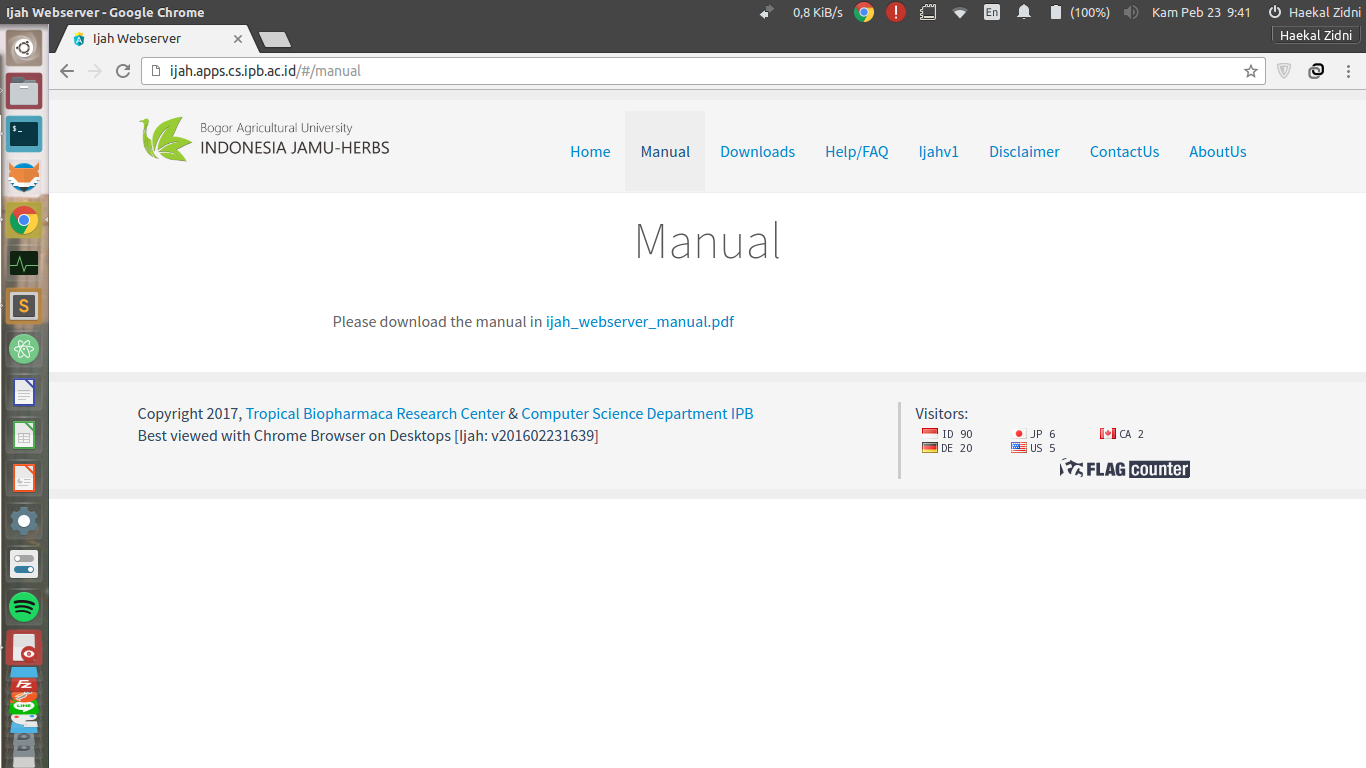
\includegraphics[scale=0.3]{ijah_manual_page.png}
% 	\caption{Halaman Manual}
% 	\label{fig:ijah_manual_page}
% \end{figure}

% \section{Downloads} \label{Downloads}

% Menu \emph{Downloads} menyediakan link untuk mengunduh Metadata seluruh item (tanaman, senyawa, protein, dan penyakit) yang ada dalam database Ijah Webserver. Juga disediakan data seluruh konektivitas (keterhubungan) antar item dan data lainnya seperti similarity data, data sekuens protein, dan lain lain.

% Untuk mengunduh file pada halaman ini cukup klik nama file yang ingin diunduh

% \begin{figure}[H]
% 	\centering
% 	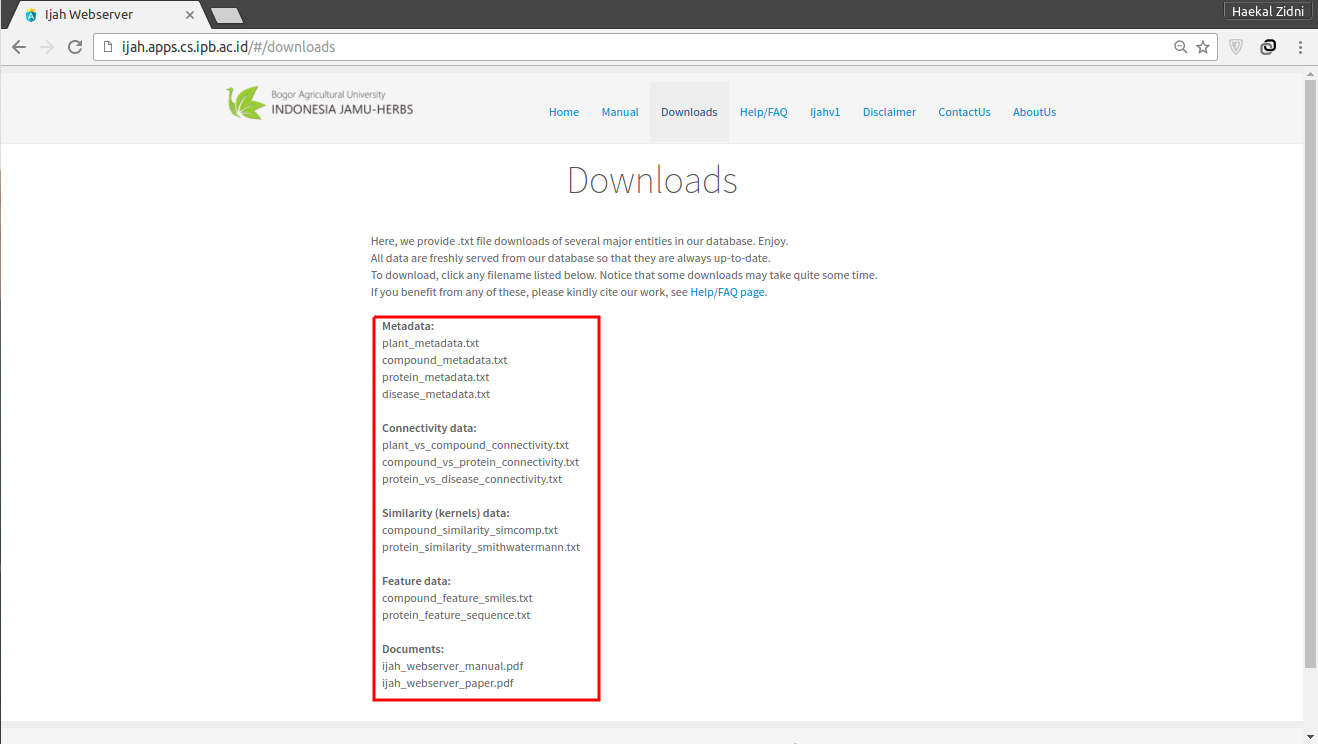
\includegraphics[scale=0.3]{ijah_downloadpage.png}
% 	\caption{Daftar file yang dapat di\-download}
% 	\label{fig:ijah_downloadpage}
% \end{figure}

% \subsection{Metadata}
% File yang dapat didownload pada kategori Metadata yaitu:

% \begin{itemize}
% \item \textbf{plant\_metadata.txt} -- Berisi metadata seluruh tanaman pada \emph{database} Ijah Webserver. 
% \item \textbf{compound\_metadata.txt} -- Berisi metadata seluruh senyawa (\emph{compound}) pada \emph{database} Ijah Webserver.
% \item \textbf{protein\_metadata.txt} -- Berisi metadata seluruh bioprotein pada \emph{database} Ijah Webserver.
% \item \textbf{disease\_metadata.txt} -- Berisi metadata seluruh penyakit pada \emph{database} Ijah Webserver.
% \end{itemize}

% \subsection{Connectivity Data}
% File yang dapat didownload pada kategori Connectivity Data yaitu:

% \begin{itemize}
% \item \textbf{plant\_vs\_compound\_connectivity.txt} -- Berisi data konektivitas tanaman dengan senyawa beserta skor konektivitasnya pada \emph{database} Ijah Webserver.
% \item \textbf{compound\_vs\_protein\_connectivity.txt} -- Berisi data konektivitas senyawa dengan protein beserta skor konektivitasnya pada \emph{database} Ijah Webserver.
% \item \textbf{protein\_vs\_disease\_connectivity.txt} -- Berisi data konektivitas protein dengan penyakit beserta skor konektivitasnya pada \emph{database} Ijah Webserver.
% \end{itemize}

% \subsection{Similarity (kernels) data}
% \begin{itemize}
% \item compound\_similarity\_simcomp.txt  
% \item protein\_similarity\_smithwatermann.txt  
% \end{itemize}

% \subsection{Feature data}
% \begin{itemize}
% \item compound\_feature\_smiles.txt  
% \item protein\_feature\_sequence.txt  
% \end{itemize}

% \subsection{Documents}
% Dokumentasi Ijah Webserver
% \begin{itemize}
% \item \textbf{ijah\_webserver\_manual.pdf} -- Manual penggunaan Ijah Webserver
% \item \textbf{ijah\_webserver\_paper.pdf} -- Paper penelitian Ijah Webserver
% \end{itemize}

% \section{Help/FAQ}
% Menu \emph{Help/FAQ} berisikan beberapa pertanyaan umum \emph{(Frequently Asked Questions)} beserta jawabannya. 

% \begin{figure}[H]
% 	\centering
% 	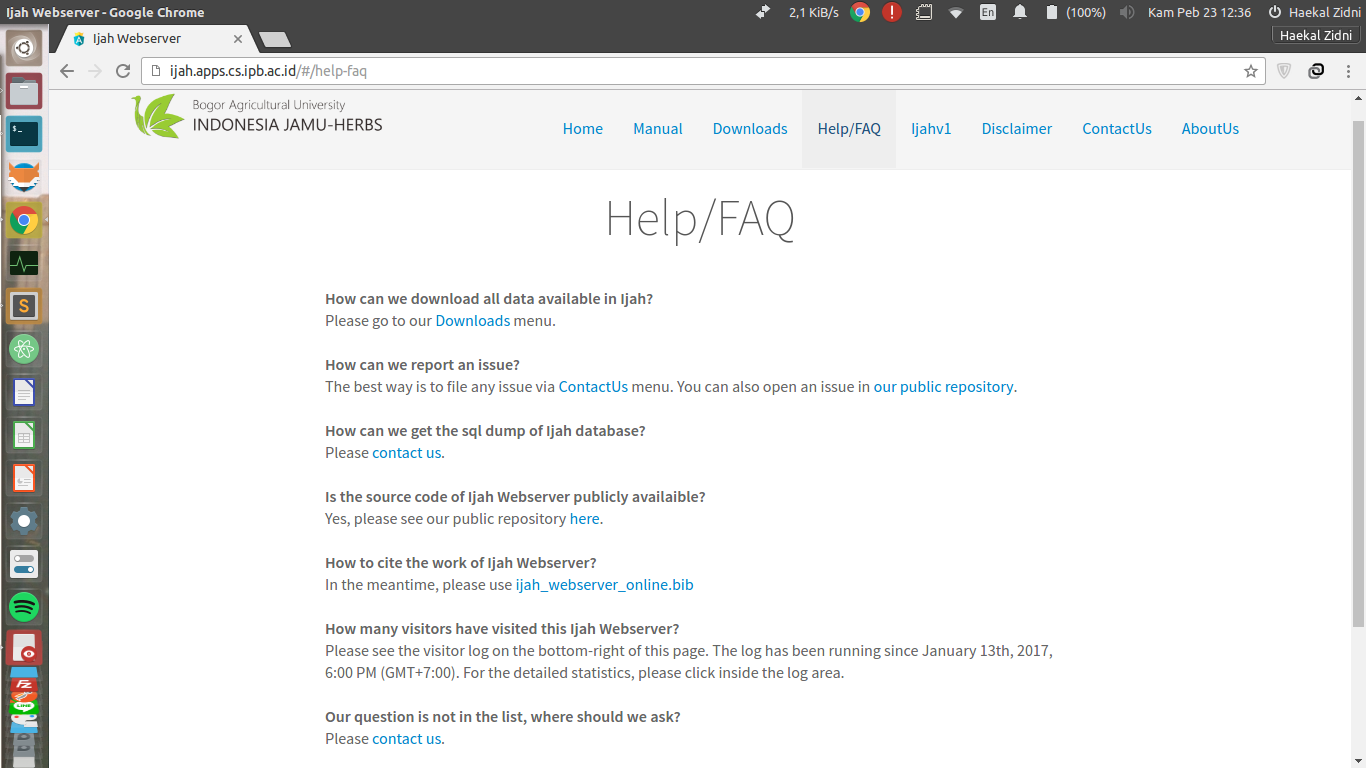
\includegraphics[scale=0.3]{ijah_faq.png}
% 	\caption{Halaman Help/FAQ}
% 	\label{fig:ijah_faq}
% \end{figure}

% Pertanyaan pertanyaan tersebut yaitu:

% \textbf{Q:} Bagaimana cara mengunduh semua data yang tersedia pada Ijah?

% A: Silakan lihat pada menu \nameref{Downloads}.

% \textbf{Q:} Bagaimana cara melaporkan isu atau galat?

% A: Silakan laporkan pada menu \nameref{Contact Us} atau pada \href{https://github.com/tttor/csipb-jamu-prj}{\emph{repository} publik kami}.

% \textbf{Q:} Bagaimana cara mendapatkan SQL dump dari database Ijah?

% A: Silakan kontak kami melalui menu \nameref{Contact Us}.

% \textbf{Q:} Apakah \emph{source code} Ijah tersedia secara publik?

% A: Ya, ada pada \href{https://github.com/tttor/csipb-jamu-prj}{\emph{repository} publik kami}.

% \textbf{Q:} Bagaimana cara mengutip dari paper Ijah Webserver?

% A: Silakan merujuk ke \href{http://ijah.apps.cs.ipb.ac.id/api/ijah_webserver_online.bib}{ijah\_webserver\_online.bib}.

% \textbf{Q:} Berapa banyak kunjungan ke Ijah Webserver?

% A: Silakan lihat \emph{visitor log} pada Footer kanan bawah, penghitungan log dimulai sejak 13 Januari 2017 pukul 18:00. Untuk lebih detail anda bisa mengklik area \emph{visitor log} tersebut.

% \textbf{Q:} Jika pertanyaan saya tidak ada pada daftar ini, dimana kami harus bertanya?

% A: Silakan kontak kami melalui menu \nameref{Contact Us}.

% \section{Ijah v1}

% Menu \emph{Ijah v1} berisi link menuju versi awal Ijah (Ijah versi 1, atau Ijah v1)

% \begin{figure}[H]
% 	\centering
% 	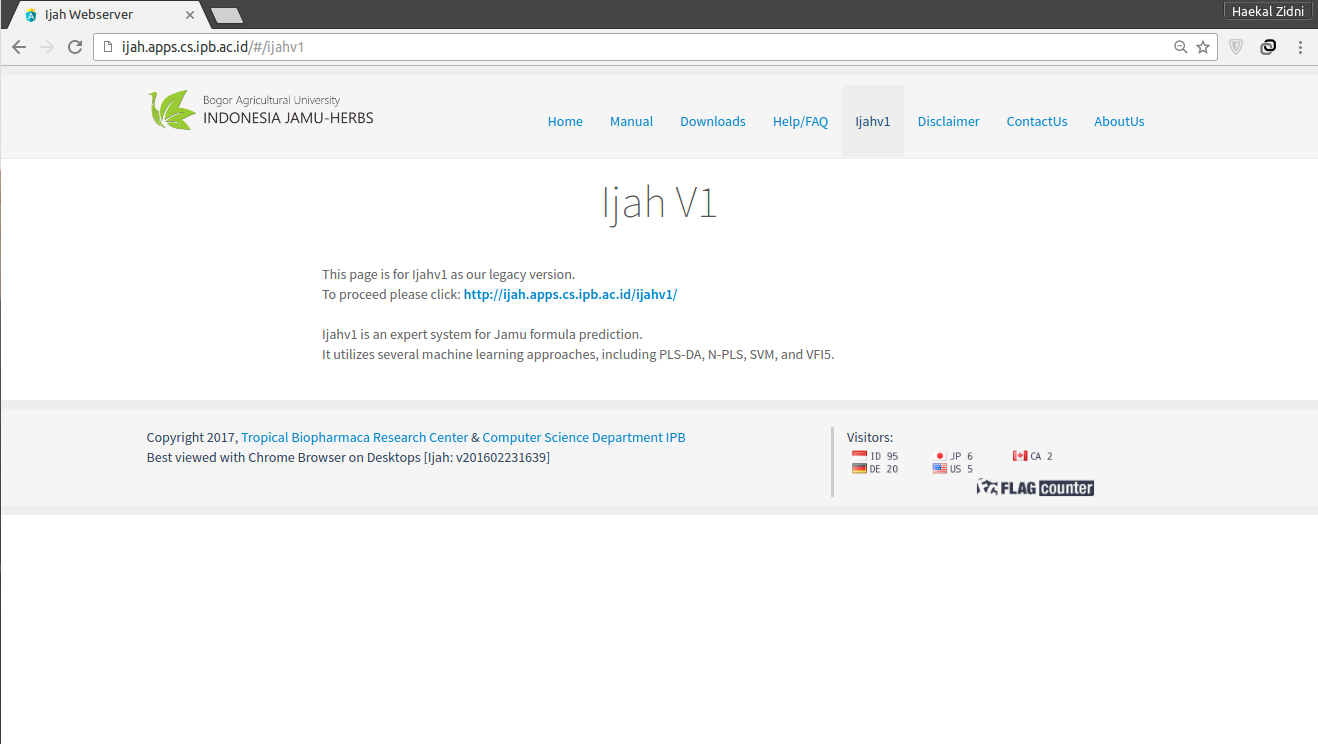
\includegraphics[scale=0.3]{ijah_v1.png}
% 	\caption{Isi halaman menu Ijah v1}
% 	\label{fig:ijah_v1}
% \end{figure}

% Jika anda ingin mengakses Ijah v1 silakan mengunjungi \url{http://ijah.apps.cs.ipb.ac.id/ijahv1/}

% \section{Disclaimer}

% Menu \emph{Disclaimer} berisikan pernyataan batasan responsibility pihak Ijah Webserver atas penggunaan hasil \emph{output} dari Ijah Webserver.

% \begin{figure}[H]
% 	\centering
% 	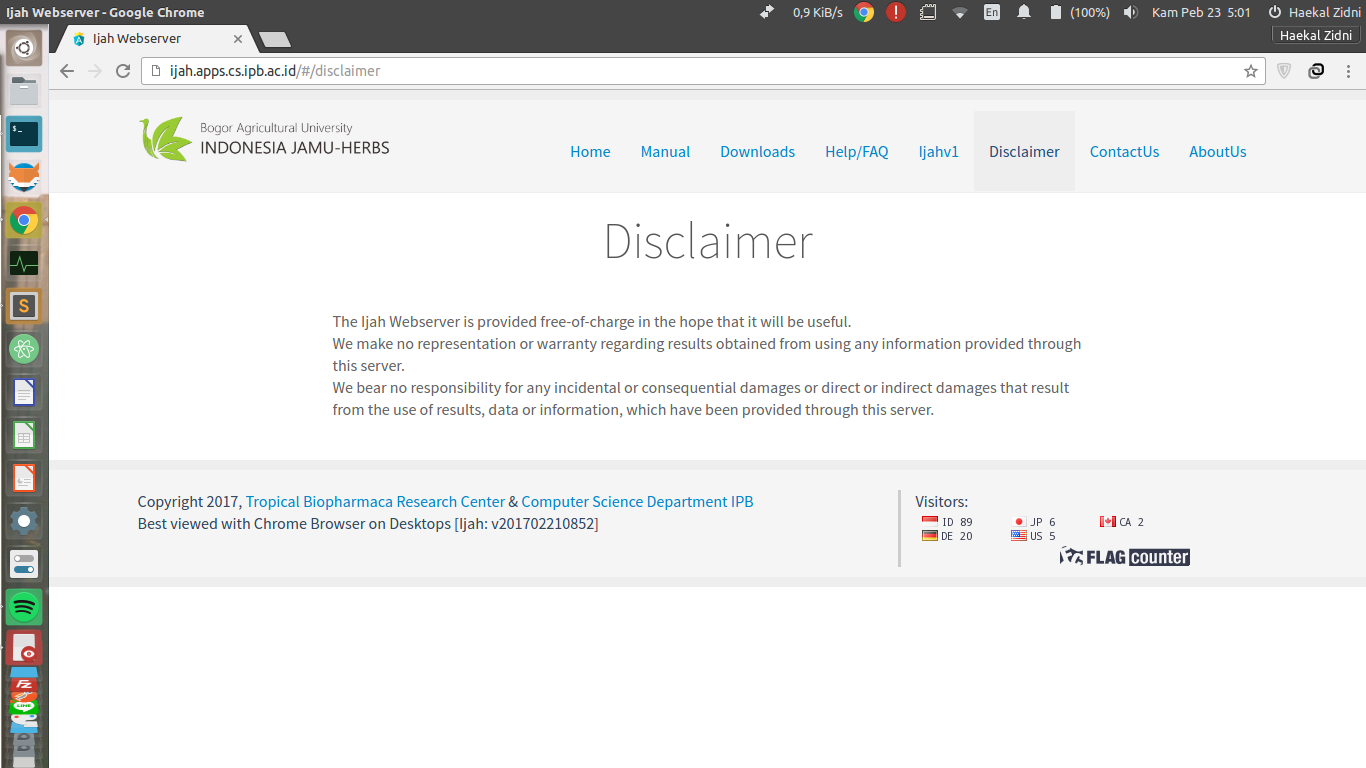
\includegraphics[scale=0.3]{ijah_disclaimer.png}
% 	\caption{Isi halaman Disclaimer}
% 	\label{fig:ijah_disclaimer}
% \end{figure}

% Di halaman ini kami menyatakan bahwa penggunaan Ijah Webserver ini gratis, dengan harapan dapat membantu banyak pihak. Namun kami tidak menjamin akibat dari penggunaan informasi dari Webserver ini. Dan kami tidak bertanggungjawab atas insiden atau kerusakan baik langsung maupun tidak langsung yang diakibatkan oleh penggunaan data atau informasi yang kami sediakan di Webserver ini.

% \section{Contact Us} \label{Contact Us}

% Menu \emph{Contact Us} merupakan sarana komunikasi antara pengguna dengan tim pengembang Ijah Webserver. Dengan mengisikan tanggapan/keluhan/saran pada form Contact Us, tanggapan anda akan terkirim ke E-mail kami.

% \begin{figure}[H]
% 	\centering
% 	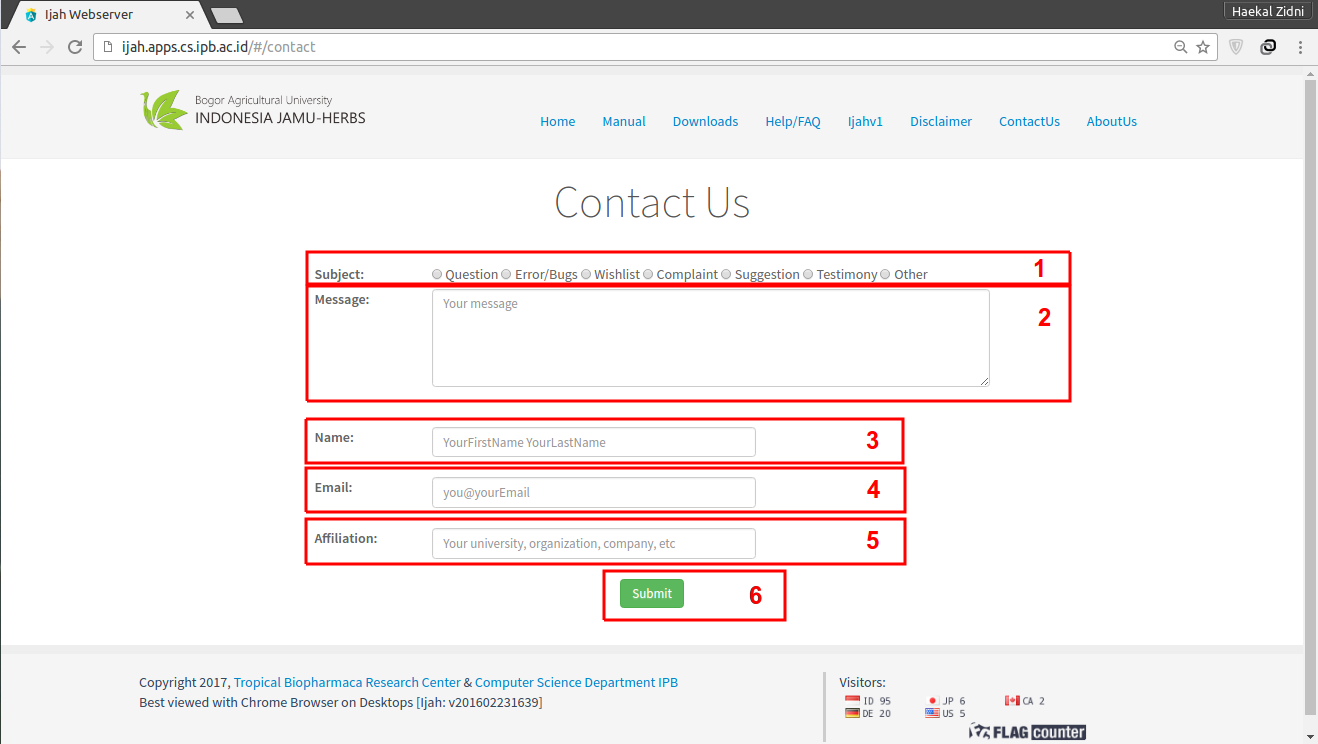
\includegraphics[scale=0.3]{ijah_contact_page.png}
% 	\caption{Halaman Contact Us pada Ijah Webserver}
% 	\label{fig:ijah_contact_page}
% \end{figure}

% \subsection{Subject}
% Pada bagian \emph{Subject} anda akan memilih jenis tanggapan anda, yaitu pertanyaan (Question), memberitahukan adanya kesalahan (Error/Bugs), menyampaikan saran fitur apa yang diinginkan pada versi selanjutnya (Wishlist), menyampaikan keluhan (Complaint), saran (Suggestion), memberikan testimoni tentang Ijah Webserver (Testimony), atau menyampaikan hal lain yang tidak termasuk dalam kategori diatas, dapat dikategorikan pada Other.

% \begin{figure}[H]
% 	\centering
% 	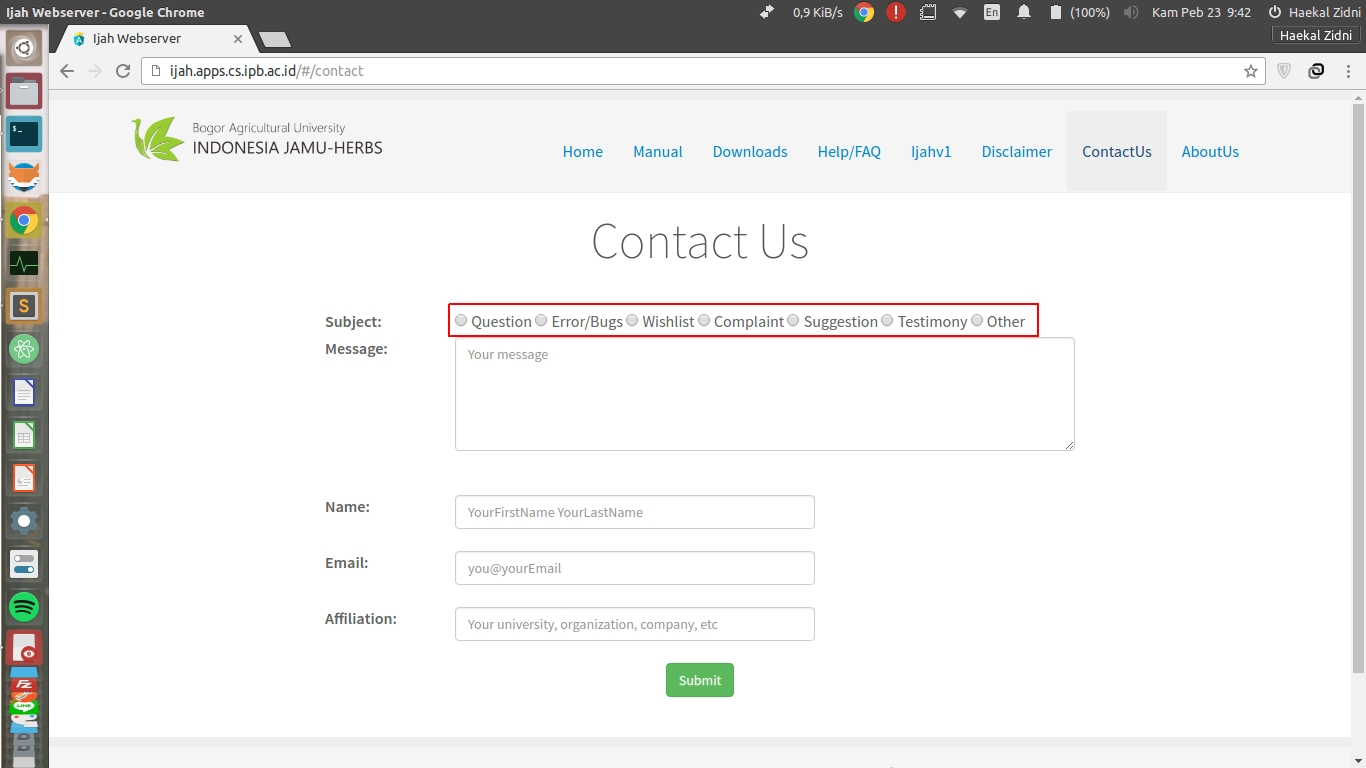
\includegraphics[scale=0.3]{ijah_contact_subject.png}
% 	\caption{Bagian \emph{Subject} pada menu Contact Us}
% 	\label{fig:ijah_contact_subject}
% \end{figure}

% \subsection{Message}
% Isikan pesan anda pada bagian \emph{Message}. Jumlah karakter tidak dibatasi, jadi mohon untuk tidak menggunakan singkatan jika tidak diperlukan demi memudahkan tim kami dalam membaca tanggapan anda. 

% \begin{figure}[H]
% 	\centering
% 	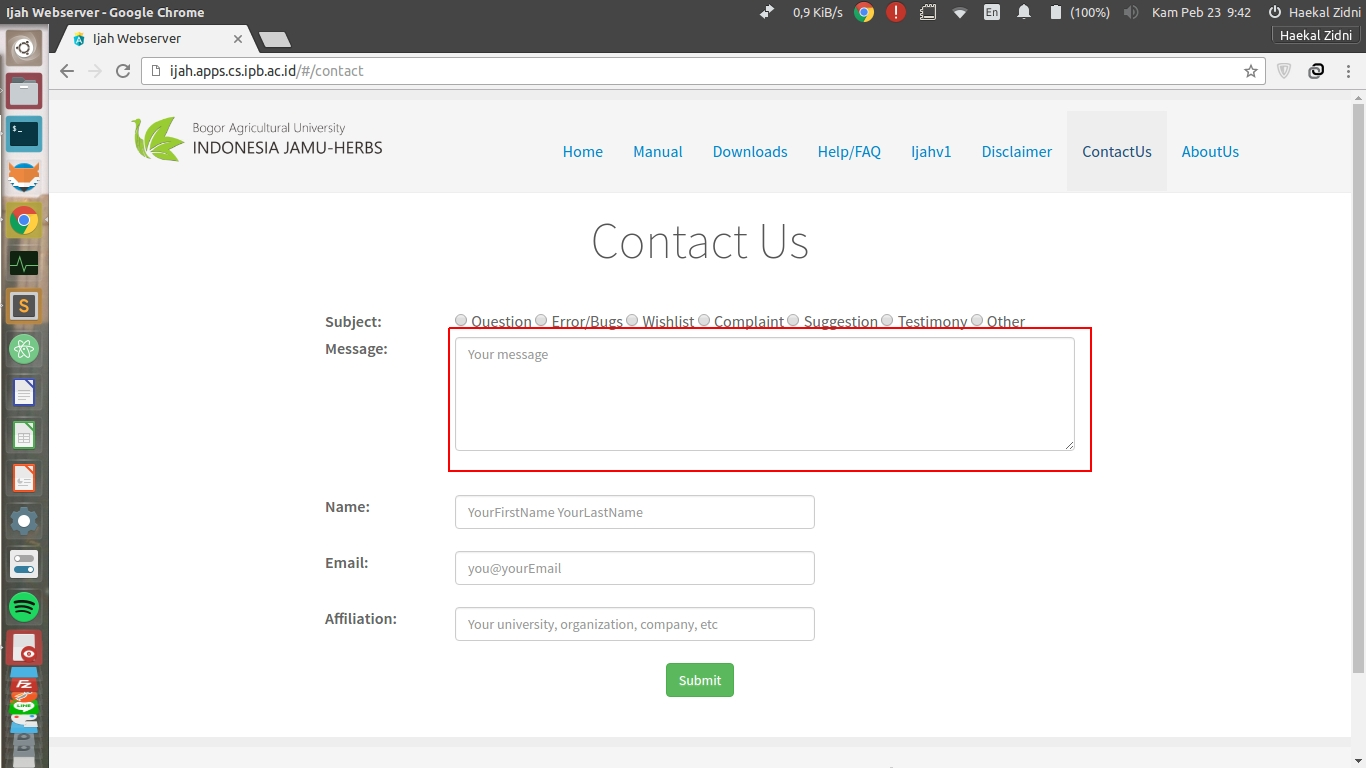
\includegraphics[scale=0.3]{ijah_contact_message.png}
% 	\caption{Bagian \emph{Message} pada menu Contact Us}
% 	\label{fig:ijah_contact_message}
% \end{figure}

% \subsection{Memasukkan Data Diri Anda}
% Setelah menuliskan tanggapan, silakan isi data diri anda, nama pada bagian \emph{Name}, alamat E\-mail anda pada bagian \emph{E\-mail}, dan afiliasi anda (organisasi, universitas, atau perusahaan) pada bagian \emph{Affiliation}.

% \textbf{Penting:} Nama dan alamat E-mail \emph{wajib} diisi. 

% \begin{figure}[H]
% 	\centering
% 	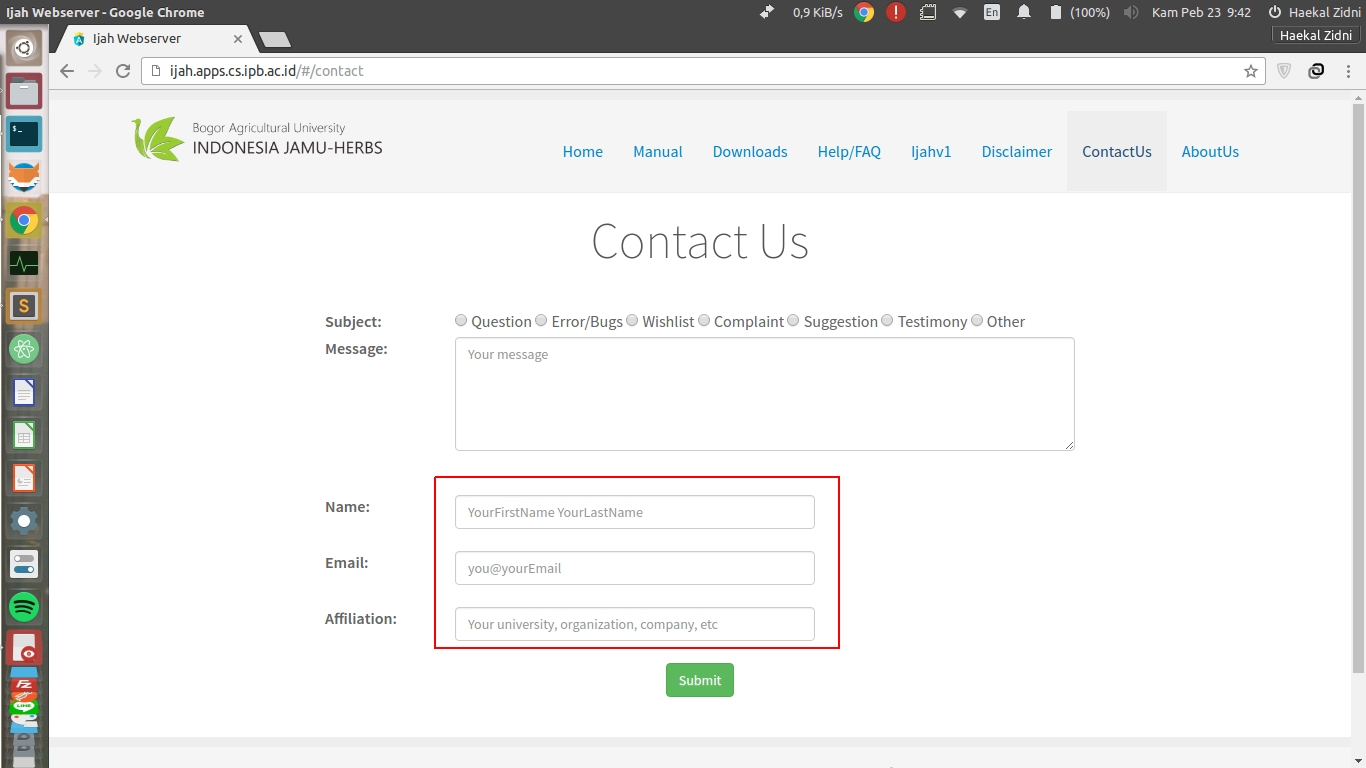
\includegraphics[scale=0.3]{ijah_contact_nameinput.png}
% 	\caption{Form pengisian nama, E-mail, dan afiliasi}
% 	\label{fig:ijah_contact_nameinput}
% \end{figure}

% Setelah terisi, tekan \textbf{Submit} dan tanggapan anda akan terkirim.

% \subsection{About Us}

% Menu \emph{About Us} berisi info tentang tim pengembang Ijah Webserver

% \begin{figure}[H]
% 	\centering
% 	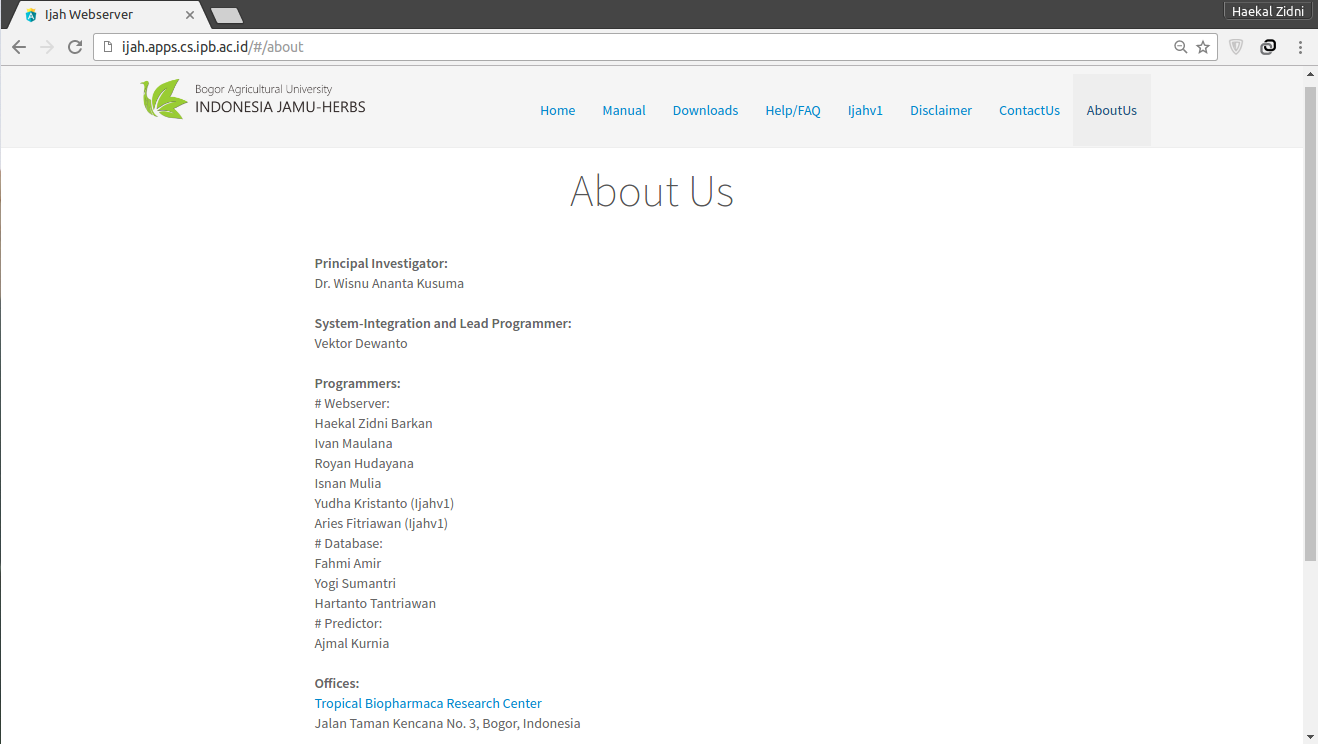
\includegraphics[scale=0.3]{ijah_about.png}
% 	\caption{Isi halaman About Us}
% 	\label{fig:ijah_about}
% \end{figure}
% %% This is an example first chapter.  You should put chapter/appendix that you
%% write into a separate file, and add a line \include{yourfilename} to
%% main.tex, where `yourfilename.tex' is the name of the chapter/appendix file.
%% You can process specific files by typing their names in at the 
%% \files=
%% prompt when you run the file main.tex through LaTeX.
\chapter{Disclaimer}



% %% This is an example first chapter.  You should put chapter/appendix that you
%% write into a separate file, and add a line \include{yourfilename} to
%% main.tex, where `yourfilename.tex' is the name of the chapter/appendix file.
%% You can process specific files by typing their names in at the 
%% \files=
%% prompt when you run the file main.tex through LaTeX.
\chapter{Rincian Anggaran Penelitian}
% Rincian anggaran penelitian mencakup jumlah dana penelitian yang dibutuhkan beserta penggunaanya
% secara wajar, namun tidak termasuk hal-hal sebagai berikut:
%  Dana untuk pembelian aset, seperti alat-alat laboratorium, komputer, dll
%  Dana honorarium
%  Dana untuk biaya perjalanan dan akomodasi (selain untuk pengambilan sampel)

% Jumlah Anggaran Total: Rp 99.500.000 \\
% Bahan habis pakai: Rp 39.500.000\\ % internet, electric power, hosting web-server, stationery
% Sewa laboratorium/alat: Rp 60.000.000 \\ % lab, computer
% Lainnya, sebutkan: Rp 0 \\

Rincian anggaran belanja untuk penelitian disajikan dalam tabel dalam gambar~\ref{fig:rab}.

\begin{figure}
	\centering
	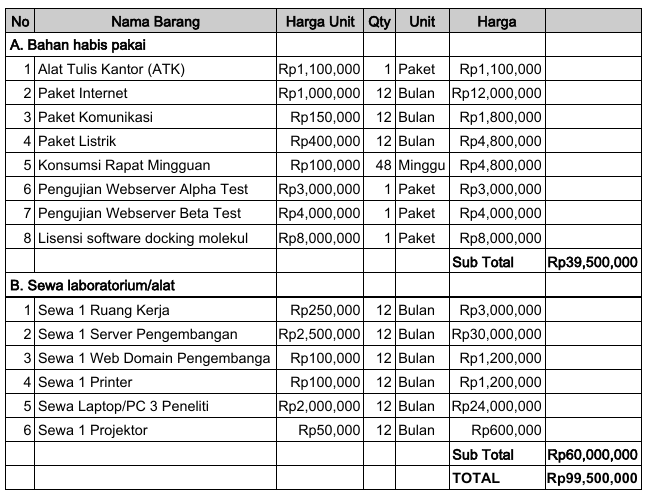
\includegraphics[scale=0.85, angle=0]{pics/rab.png}
	% \includegraphics[width=\columnwidth]{pics/timeline.png}
 	\caption{Rincian anggaran belanja untuk penelitian.}
  	\label{fig:rab}
\end{figure}  
%\printbibliography
%
% Daftar Pustaka
%\include{pustaka}
%biblama (bukan biblatex)
% \bibliography{main, isnan}{}
%\bibliography{references}{}
%biblama (bukan biblatex)
% \bibliographystyle{apalikerd}
% \bibliographystyle{apa}
%\bibliographystyle{ieeetr}

\begin{singlespace}
	\bibliography{main}
	% \bibliographystyle{apa}
	\bibliographystyle{plain}
\end{singlespace}



% % Lampiran 
% \begin{appendix}
% 	%
% @author  Andreas Febrian
% @version 1.00 
% 
% Hanya sebuah pembatas bertuliskan LAMPIRAN ditengah halaman. 
% 

\begin{titlepage}
	\centering 
	\vspace*{6cm}
	\noindent \Huge{LAMPIRAN}
	\addChapter{LAMPIRAN}
\end{titlepage}
% 	\setcounter{page}{2}
% 	% %-----------------------------------------------------------------------------%
\addChapter{Lampiran 1 : Kode Sumber}
\chapter*{Lampiran 1 : Kode Sumber}
%-----------------------------------------------------------------------------%
\section*{\code{admin\_useraddmaster}} \label{cha:lampir-admin}
Skrip ini diletakkan pada direktori \co{/usr/sesuatu} dan hanya dapat dieksekusi oleh \f{root}. Skrip ini berguna untuk menambahkan pengguna baru sesuai dengan konfigurasi baru yang telah ditetapkan.
\begin{lstlisting}[style=L,caption={Skrip menambahkan pengguna baru},label={lst:adduser}]
#!/bin/csh -f
blah blah blah
blah blah blah
blah blah blah
blah blah blah
blah blah blah
\end{lstlisting}

\section*{\code{getuser.cron}} \label{cha:lampir-cronadmin}
Penjelasan skrip disini
\begin{lstlisting}[style=L,caption={\f{Cronjob} menambahkan pengguna baru},label={lst:cronadduser}]
#!/bin/bash
# Change these two lines to localize to your system:
# Adapted from /usr/local/sbin/admin_useradd

cat /dev/null > $userlist
for (( i=0; i<${#listemailto[@]}; i++ ))
do
        uname=${listusername[$i]}
        mailto=${listemailto[$i]}

        echo "User $uname created, please use torqace wisely." | mail -s "Torqace user registration" $mailto
done

\end{lstlisting}

%-----------------------------------------------------------------------------%
\addChapter{Lampiran 2 : Berkas Konfigurasi}
\chapter*{Lampiran 2 : Berkas Konfigurasi}
%-----------------------------------------------------------------------------%
\section*{compute.xml}
\begin{lstlisting}[caption={Berkas \co{compute.xml}},label={lst:excomp},language=XML]
<?xml version="1.0" standalone="no"?>
<kickstart>
<description>
	Compute node XML file
</description>
</kickstart> 
\end{lstlisting}

%-----------------------------------------------------------------------------%
\addChapter{Lampiran 8 : UAT dan Kuesioner}
%-----------------------------------------------------------------------------%
\begin{landscape}
\chapter*{Lampiran 8 : UAT dan Kuesioner}
\begin{longtable}{|c|p{7cm}|p{2.5cm}|p{3.5cm}|p{3.3cm}|p{1.8cm}|}
\caption{Tabel UAT dan Kuesioner} \label{tab:uattbl}\\
\hline
No. & \multicolumn{1}{c|}{Langkah Penggunaan} & Fitur Berjalan & Tingkat Kemudahan (1-5) & Tingkat Kepuasan (1-5) & Saran / Komentar \\ 
\cline{3-5} & & Berhasil /Tidak & 1:Sangat sulit ; \hspace{100pt} 5:sangat mudah & 1 : Sangat kecewa ; 5 : sangat puas &  \\ \hline
\multicolumn{ 6}{|>{\columncolor{headertbl}}c|}{Use Case : Login} \\ \hline
1.1 & Pengguna berada pada halaman depan torqace &  &  &  &  \\ \hline
1.2 & Pengguna memasukkan username dan password pada field yang telah disediakan.Kemudian menekan tombol 'login' &  &  &  &  \\ \hline
1.3 & Apabila Sukses, maka pengguna masuk ke dalam sistem dan dihadapkan pada menu utama &  &  &  &  \\ \hline
\multicolumn{ 6}{|>{\columncolor{headertbl}}c|}{Use Case : Register} \\ \hline
2.1 & Pengguna berada pada halaman registrasi pengguna torqace &  &  &  &  \\ \hline
2.2 & Pengguna memasukkan username,password, dan email pada field yang telah disediakan. Kemudian menekan tombol 'submit' &  &  &  &  \\ \hline
2.3 & Sistem akan mengonfirmasi masukan, dan akan mengirimkan email untuk memberitahu pengguna apabila proses pendaftaran telah selesai &  &  &  &  \\ \hline
\multicolumn{ 6}{|>{\columncolor{headertbl}}c|}{Use Case : Logout} \\ \hline
3.1 & Pengguna memilih menu untuk melakukan logout &  &  &  &  \\ \hline
3.2 & Sistem akan mengeluarkan pengguna, dan pengguna tidak dapat menggunakan fitur-fitur utama aplikasi &  &  &  &  \\ \hline
\multicolumn{ 6}{|>{\columncolor{headertbl}}c|}{Use Case : Upload Job Sederhana} \\ \hline
4.1 & Pengguna memilih menu upload file/project pada menu utama &  &  &  &  \\ \hline
4.2 & Pengguna memilih pilihan 'single file' pada tipe project &  &  &  &  \\ \hline
4.3 & Pengguna memilih berkas yang akan diunggah, mengisi label, dan menentukan apakah akan menimpa project sebelumnya dengan nama yang sama atau tidak &  &  &  &  \\ \hline
4.4 & Pengguna menekan tombol 'submit' dan mengonfirmasi  &  &  &  &  \\ \hline
4.5 & Sistem akan menampilkan informasi terkait berkas yang diupload &  &  &  &  \\ \hline
\multicolumn{ 6}{|>{\columncolor{headertbl}}c|}{Use Case : Upload Job Compressed} \\ \hline
5.1 & Pengguna memilih menu upload file/project pada menu utama &  &  &  &  \\ \hline
5.2 & Pengguna memilih pilihan 'compressed files' pada tipe project &  &  &  &  \\ \hline
5.3 & Pengguna memilih arsip yang akan diunggah, mengisi label, menentukan akan melakukan make atau tidak dan menentukan apakah akan menimpa project sebelumnya dengan nama yang sama atau tidak &  &  &  &  \\ \hline
5.4 & Pengguna menekan tombol 'submit' dan mengonfirmasi  &  &  &  &  \\ \hline
5.5 & Sistem akan menampilkan informasi terkait berkas yang diupload dan diekstrak. Keluaran make juga akan ditampilkan bila dipilih &  &  &  &  \\ \hline
\multicolumn{ 6}{|>{\columncolor{headertbl}}c|}{Use Case : Upload Array Job} \\ \hline
6.1 & Pengguna memilih menu upload file/project pada menu utama &  &  &  &  \\ \hline
6.2 & Pengguna memilih pilihan 'array' pada tipe project &  &  &  &  \\ \hline
6.3 & Pengguna memilih arsip-arsip yang akan diunggah, mengisi label, menentukan akan melakukan make atau tidak dan menentukan apakah akan menimpa project sebelumnya dengan nama yang sama atau tidak &  &  &  &  \\ \hline
6.4 & Pengguna menekan tombol 'submit' dan mengonfirmasi  &  &  &  &  \\ \hline
6.5 & Sistem akan menampilkan informasi terkait berkas yang diupload dan diekstrak. Keluaran make juga akan ditampilkan bila dipilih &  &  &  &  \\ \hline
\multicolumn{ 6}{|>{\columncolor{headertbl}}c|}{Use Case : Melihat antrian pada queue} \\ \hline
7.1 & Pengguna memilih menu  queue status pada menu utama &  &  &  &  \\ \hline
7.2 & Pengguna berada pada halaman yang berisi informasi queue &  &  &  &  \\ \hline
\multicolumn{ 6}{|>{\columncolor{headertbl}}c|}{Use Case : Melihat detil antrian} \\ \hline
8.1 & Dari halaman status queue, pengguna memilih job tertentu &  &  &  &  \\ \hline
8.2 & Informasi mengenai detil job tersebut ditampilkan dalam bentuk tabel &  &  &  &  \\ \hline
8.2.1 & Apabila job tersebut bukan milik pengguna, maka sistem akan melarang pengguna melihat informasi detil suatu job &  &  &  &  \\ \hline
\multicolumn{ 6}{|>{\columncolor{headertbl}}c|}{Use Case : Membuat script job} \\ \hline
9.1 & Pengguna memilih untuk melakukan 'generate script' baik dari laporan upload berkas, atau dari penjelajahan direktori &  &  &  &  \\ \hline
9.2 & Pengguna mengisi nama job, parameter job, dan script yang akan dijalankan.  &  &  &  &  \\ \hline
9.3 & Pengguna mengonfirmasi konfirmasi submit job &  &  &  &  \\ \hline
9.4 & Pengguna dapat melihat informasi script secara keseluruhan dan pesan apakah terjadi kegagalan atau tidak, serta id job yang diberikan &  &  &  &  \\ \hline
\multicolumn{ 6}{|>{\columncolor{headertbl}}c|}{Use Case : Load spesifikasi job lain} \\ \hline
10.1 & Pengguna berada pada halaman untuk membuat script &  &  &  &  \\ \hline
10.2 & Pengguna memilih 'Load a Previous Job' &  &  &  &  \\ \hline
10.3 & Pengguna memilih job mana yang akan dimuat dan menekan tombol 'Load' &  &  &  &  \\ \hline
10.4 & Pengguna kembali ke halaman pembuatan script dengan spesifikasi job sebelumnya &  &  &  &  \\ \hline
\multicolumn{ 6}{|>{\columncolor{headertbl}}c|}{Use Case : Menjelajah Direktori} \\ \hline
11.1 & Pengguna memilih menu  'View File/Project'  pada menu utama &  &  &  &  \\ \hline
11.2 & Pengguna dapat melakukan navigasi untuk masuk ke dalam direktori tertentu, atau kembali ke direktori diatasnya, dan dapat melihat terdapat berkas apa saja dalam direktori &  &  &  &  \\ \hline
\multicolumn{ 6}{|>{\columncolor{headertbl}}c|}{Use Case : Menghapus Berkas/Direktori} \\ \hline
12.1 & Pengguna berada pada halaman penjelajahan direktori &  &  &  &  \\ \hline
12.2 & Pengguna memilih pilihan untuk menghapus berkas/direktori di samping item yang akan dihapus &  &  &  &  \\ \hline
12.3 & Pengguna mengonfirmasi konfirmasi penghapusan &  &  &  &  \\ \hline
\multicolumn{ 6}{|>{\columncolor{headertbl}}c|}{Use Case : Mengunduh Berkas/Direktori} \\ \hline
13.1 & Pengguna berada pada halaman penjelajahan direktori &  &  &  &  \\ \hline
13.2 & Pengguna memilih pilihan untuk mengunduh berkas/direktori di samping item yang akan dihapus &  &  &  &  \\ \hline
\multicolumn{ 6}{|>{\columncolor{headertbl}}c|}{Use Case : Melihat Berkas} \\ \hline
14.1 & Pengguna berada pada halaman penjelajahan direktori &  &  &  &  \\ \hline
14.2 & Pengguna memilih berkas yang berupa berkas teks &  &  &  &  \\ \hline
14.3 & Sistem akan menampilkan konten dari berkas tersebut &  &  &  &  \\ \hline
\end{longtable}
\end{landscape}
% \end{appendix}

\end{document}
